\documentclass[a4paper,11.5pt]{report}
\usepackage[margin=0.4in]{geometry}
\usepackage{hyperref}
\usepackage{setspace}
\usepackage{lastpage}
\usepackage{tabularx}


  % Preamble packages:
\usepackage{booktabs}
\usepackage{multirow}
\usepackage{caption}




\usepackage{multicol}
\usepackage{caption}

% for apa with apa
% \usepackage{natbib} 
% for ieee with IEEEtran
\usepackage[numbers]{natbib}
\usepackage{float}
\usepackage{grffile}  % Add to preamble
\usepackage{titlesec} % Add this line for chapter formatting

\usepackage{graphicx}

\usepackage{float} % If you use [H] placement


% Required in preamble
\usepackage{pgfplots}      % Core plotting package
\pgfplotsset{compat=1.18} % Set compatibility mode (use newest version available) % For general graphics handling (usually auto-loaded)

% Required packages in preamble
\usepackage{algorithm}      % For algorithm float environment
\usepackage{algpseudocode}  % For algorithmic structure (functions, loops, etc.)
\usepackage{xspace}         % For smart spacing after macros (optional but recommended)

\usepackage{csquotes}

\renewcommand{\familydefault}{\sfdefault}
\usepackage{helvet}
\usepackage{amsmath}
\usepackage{tikz}
\usetikzlibrary{positioning}

\renewcommand{\contentsname}{Table of Contents}


\usepackage{booktabs} % For professional quality tables
\usepackage{caption}  % For captions of figures and tables
\usepackage{subcaption} % For subfigures within a figure environment
% \usepackage[backend=biber, style=apa]{biblatex} % Example for bibliography (if needed, adapt style)
% \addbibresource{references.bib} % Link to your bibliography file
% \usepackage{hyperref} % Optional: for clickable links and references
% \usepackage[capitalise]{cleveref} % Optional: for smart cross-referencing (e.g., Figure 1, Table 2)

\usepackage{pgffor}
% MAKE Smaller
% make lists small
\usepackage{enumitem}
\setlist{nosep} % Removes extra space in itemize/enumerate

\titlespacing*{\section}{0pt}{0.5em}{0.5em}
\titlespacing*{\subsection}{0pt}{0.5em}{0.5em}


\setlength{\parindent}{1.5em}
\setlength{\parskip}{0.5em} % Adjust spacing between paragraphs

% Customise hyperlink appearance (Optional)
\hypersetup{
    colorlinks=true,        % Enable colored links
    linkcolor=black,        % Color for internal links (TOC, sections, etc.)
    citecolor=black,        % Color for citation links
    filecolor=black,        % Color for file links
    urlcolor=blue          % Color for external URLs
}

% \titleformat{\chapter}[hang]{\normalfont\huge\bfseries}{\thechapter.}{0.5em}{}

\titleformat{\chapter}[display]
  {\normalfont\Huge\bfseries}
  {}
  {0pt}
  {\vspace{-2em}}
\titlespacing*{\chapter}{0pt}{-2em}{1em}


\begin{document}

% % Cover Page
% \begin{titlepage}
%     \begin{center}

%         \textbf{\LARGE{School of Computer Science}}\\[0.5em]
%         \textbf{\Large{Faculty of Science and Engineering}}\\[0.5em]
%         \textbf{\Large{University of Nottingham}}\\[0.5em]
%         \textbf{\Large{Malaysia}}\\[5em]

%         
\includegraphics[width=0.5\textwidth]{images/nottingham_logo.png}\\[3em]

%         \textbf{\Large{UG FINAL YEAR DISSERTATION REPORT}}\\[6em]
%         \textbf{\large{\textit{Interpretable Seagull classification}}}\\[6em]

%     \end{center}

%     \begin{center}
%         \begin{minipage}{0.6\textwidth}  % adjust width as needed
%             \raggedright
%             \textbf{Student's Name} \hspace{1.5cm}: Aravindh Palaniguru\\[1em]
%             \textbf{Student Number} \hspace{1.4cm}: 20511833\\[1em]
%             \textbf{Supervisor Name} \hspace{1.2cm}: Dr. Tomas Maul\\[1em]
%             \textbf{Year} \hspace{3.8cm}: 2025\\[4em]
%         \end{minipage}
%     \end{center}

%     \vfill

%     \begin{center}
%         \begin{minipage}{\textwidth}
%             \centering
%             {\fontsize{12}{10}\selectfont\textbf{SUBMITTED IN PARTIAL FULFILLMENT OF THE REQUIREMENTS FOR THE AWARD OF}}
%             {\fontsize{12}{10}\selectfont\textbf{BACHELOR OF SCIENCE IN COMPUTER SCIENCE WITH ARTIFICIAL INTELLIGENCE (HONS)}}\\
%             {\fontsize{12}{10}\selectfont\textbf{THE UNIVERSITY OF NOTTINGHAM}}
%         \end{minipage}
%     \end{center}
% \end{titlepage}

% % Title Page
% \newpage
% \begin{titlepage}
%     \begin{center}
%         \vspace{0.1em}
%         
\includegraphics[width=0.5\textwidth]{images/nottingham_logo.png}\\[6em]

%         \textbf{INTERPRETABLE SEAGULL CLASSIFICATION}\\[6em]

%         \fontsize{10}{10}{Submitted in May 2025, in partial fulfillment of the conditions of the award of the degrees B.Sc.}\\[4em]

%         Aravindh Palaniguru\\
%         School of Computer Science\\
%         Faculty of Science and Engineering\\
%         University of Nottingham\\
%         Malaysia\\[6em]

%         I hereby declare that this dissertation is all my own work, except as indicated in the text:\\[4em]

%         Signature \underline{\hspace{7cm}}\\[2em]
%         Date \hspace{1cm} \underline{\hspace{1cm}} / \underline{\hspace{1cm}} / \underline{\hspace{2cm}}
%     \end{center}
% \end{titlepage}

% Change margins for Table of Contents and subsequent pages
\newgeometry{
    margin=1in
}

% Roman numbering for preliminary pages
\pagenumbering{roman}

% % Acknowledgement
% \newpage
% \section*{\centering \normalsize{Acknowledgement}}

% % Abstract
% \newpage
% \section*{\centering \normalsize{Abstract}}


% Table of Contents
\newpage
\tableofcontents

% % List of Figures
% \newpage
% \listoffigures

% % List of Tables
% \newpage
% \listoftables

% Switch to Arabic numbering starting from Introduction
\newpage
\cleardoublepage % Ensure proper page break before switching numbering style
\pagenumbering{arabic} % Switch to Arabic numerals
\setcounter{page}{1} % Restart page numbering at 1

% Introduction
\chapter{Introduction}

Biodiversity is under unprecedented pressure due to climate change and human influence. The alarming rates at which species are disappearing indicate that the sixth mass extinction is underway \citep{Ceballos2017}. Understanding what biodiversity we have and what we stand to lose is crucial for convincing decision-makers to take appropriate conservation action. The gaps in taxonomic knowledge and shortage of experts constitute what is known as the "taxonomic impediment" \citep{taxonomicimpediment}, which hampers our ability to document and protect biodiversity effectively. Determining whether two populations can be consistently distinguished based on morphological traits remains essential for establishing taxonomic boundaries and designing appropriate conservation strategies.

Birds are frequently utilized to assess environmental quality due to their sensitivity to ecological changes and ease of observation during field studies. Researchers often rely on bird diversity as an indicator of the diversity within other species groups and the overall health of human environments. Examples include monitoring environmental changes through bird population shifts, tracking climate change via bird migration patterns, and evaluating biodiversity by counting bird species. Accurate identification of bird species is essential for detecting species diversity and conserving rare or endangered birds promoting scientific research and conservation efforts.\citep{ani13020264}

Among birds, gulls (\textit{Laridae}) present a particularly challenging case for identification due to their recent evolutionary divergence and subtle morphological differences. The wing and wingtip patterns—particularly the colour, intensity, and pattern of the primary feathers—are crucial diagnostic features for identification, yet they exhibit considerable variation within each species. 
%TODO CHECK FEATURES

The classification of gulls presents multiple challenges that make traditional identification methods problematic and inconsistent.
Multiple confounding factors complicate identification \citep{adriaens2022}:
\begin{itemize}
    \item \textbf{Hybridization:} Species can interbreed in overlapping ranges, creating intermediate forms.
    \item \textbf{Age-related variations:} Juvenile and immature gulls display less distinct patterns than adults.
    \item \textbf{Environmental effects:} Feather bleaching from sun exposure, contamination, and wear can alter appearance.
    \item \textbf{Seasonal moulting:} Gulls undergo plumage changes throughout the year, affecting diagnostic features.
    \item \textbf{Viewing conditions:} Lighting, angle, and distance significantly impact observed coloration.
\end{itemize} 

As noted by ornithologists:

\begin{quote}
    ``Gulls can be a challenging group of birds to identify. To the untrained eye, they all look alike, yet, at the same time, in the case of the large gulls, one could say that no two birds look the same!'' \citep{ayyash2024}.
\end{quote}

This project addresses the multifaceted challenge of fine-grained analysis between two closely related gull species: the Slaty-backed Gull and the Glaucous-winged Gull. These species, found primarily in eastern Russia and the Pacific Coast of the USA, display subtle and overlapping physical characteristics that make accurate identification highly complex.

\begin{quote}
    Glaucous-winged Gulls also exhibit variably pigmented wingtips... these differences are often chalked up to individual
    variation, at least by this author, but they're inconveniently found in several hybrid zones, creating potential for much
    confusion.
    
    The amount of variation here is disturbing because it is unmatched by any other gull species, and more so because it is not completely understood \citep{adriaens2022gulls}.
\end{quote}

There are many methods that can be used for classification. Manual identification to classify species requires per specimen analysis by expert taxonomists which is time consuming. Automated taxon identification systems (ATIs) could both handle routine identifications and potentially assist in identifying new species. Traditional ATIs, however, have been limited by their reliance on hand-crafted features \citep{valan}, are time-consuming hindering large-scale surveys, making them difficult to generalize across different taxonomic groups. As mentioned by \citep{Lu2024}, "While using machine learning techniques to solve the problem of fine-grained classification, traditional feature extraction methods necessitate manually designed features, such as edge detection, color histograms, feature point matching, and visual word bags, which have limited expressive capabilities and require extensive annotation details like bounding boxes and key points. The drawback of these methods lies in the extensive manual intervention required for feature selection and extraction."

Fine-grained image classification (FGIC), which focuses on identifying subtle differences between subclasses within the same category, has advanced rapidly over the past decade with the development of sophisticated deep neural network architectures. Deep learning approaches offer promising solutions to this taxonomic challenge through their ability to automatically learn discriminative features from large datasets\citep{source4}. 

Unlike traditional machine learning methods that rely on hand-engineered features, deep neural networks can detect complex patterns in high-dimensional data, making them well-suited for fine-grained visual classification tasks~\citep{valan}. Features extracted through convolution are learned automatically by multilayer convolutional neural networks, offering the model greater adaptability to various tasks and datasets, with features possessing enhanced expressive and abstract capabilities. The benefit of convolutional feature extraction is its ability to perform feature extraction and classification within the same network, with the quality and quantity of features adjustable through the network's structure and parameters \citep{source2} offering the model greater adaptability to various tasks and datasets \citep{Lu2024}. Getting good quality results in traditional machine Learning models is dependent on how good the data is labelled, whereas Deep Learning architectures don't necessarily require labelling, as Neural Networks are great at learning without guidelines~\cite{source5}.
%TODO check references



As demonstrated in comparative studies, 

For species identification specifically, convolutional neural networks (CNNs) such as ResNet, Inception, and VGG have demonstrated exceptional capabilities \cite{essay101313}, with recent studies such as \citep{transferln97} who mentioned that "deep learning is more effective than traditional machine learning algorithms in image recognition as the number of bird species increases" achieving accuracy rates exceeding 97\% in bird species classification tasks. \citep{ALFATEMI2024558} compared deep learning and traditional machine learning algorithms achieved high accuracy of 94\% tackle the challenge of classifying bird species with high visual similarity and subtle variations. These architectures automatically learn hierarchical feature representations—from low-level edges and textures to high-level semantic concepts—that capture the subtle morphological differences between closely related species.

Yet the fine-grained bird classification task has greater challenges even when using deep learning  \cite{source3} \citep{ani13020264}.
\begin{enumerate}
    \item High intraclass variance. Birds belonging to the same category usually present distinctly different postures and perspectives.
    \item Low inter-class variance. Some of the different categories of birds may have only minor differences; for example, some of the differences are only in the color pattern on the head.
    \item Limited training data. Some bird data are limited in number, especially endangered species, for whom it is difficult to collect sufficient image data. Meanwhile, the labeling of bird categories usually requires a great deal of time by experts in the corresponding fields. These problems greatly increase the difficulty of acquiring training data.
    \item Large intensity variation in images as pictures are taken in different time of a day (like morning, noon, evening etc.).
    \item Various poses of Bird (like flying, sitting with different orientation).
    \item Bird localization in the image as there are some images in which there are more than one bird in that image.
    \item Large Variation in Background of the images.
    \item Various type of occlusions of birds in the images (leaf or branches of the tree).
    \item Size or portion of the bird covered in the images.
    \item Less no of sample images per class and also class imbalance \citep{10.1007/978-981-15-1387-9_3}.
    \item Deep Learning requires an abundant amount of data in order to produce accurate results.
    \item Overfitting is a prevalent problem in Deep Learning and can sometimes negatively affect the model performance in real-time scenarios.
\end{enumerate}

This project aims to develop and evaluat deep learning models for automated classification. Additionally, this research focuses on uncovering and analyzing the most influential features that distinguish these two gull species. Interpretability mechanisms such as Grad-CAM (Gradient-weighted Class Activation Mapping) is used to visualize and interpret the regions and morphological traits that deep neural networks prioritize during classification. Complementing this, statistical analysis and unsupervised clustering methods are employed to quantitatively assess which visual features most effectively separate the species, further validating the biological relevance of the model's learned features. By doing so, this project not only seeks to achieve high classification accuracy, but also aims to provide interpretable insights into the distinguishing characteristics of each gull species. This dual approach bridges ecology and computer science, increasing both the practical utility and scientific transparency of AI-powered biodiversity monitoring.

% Related Work
\newpage
\chapter{Literature Review}
\section*{Deep Learning for Fine-Grained Image Classification}
Fine-grained image classification presents unique challenges compared to general image classification tasks. Fine-grained classification \enquote{necessitates discrimination between semantic and instance levels, while considering the similarity and diversity among categories} \citep{source2}. This is particularly challenging in bird classification due to three key factors: high intra-class variance (birds of the same species in different postures), low inter-class variance (different species with only minor differences), and limited training data availability, especially for rare species\citep{source2}.

Early approaches to fine-grained classification relied on fixed rectangular bounding boxes and part annotations to obtain visual differences, but these methods required extensive human annotation effort. Recent research has shifted toward weakly supervised approaches that only require image-level labels, developing localization subnetworks to identify critical parts followed by classification subnetwork. \citep{source2} These models facilitate learning while maintaining high accuracy without needing pre-selected boxes, making them more practical for real-world applications.

% Recent research emphasizes that effective fine-grained classification depends on identifying and integrating information from multiple discriminative regions rather than focusing on a single region. As highlighted in recent literature, "it is imperative to integrate information from various regions rather than relying on a singular region"\href{https://www.frontiersin.org/journals/neurorobotics/articles/10.3389/fnbot.2024.1391791/full}{4}. This insight has led to the development of methods combining features from different levels via attention modules, thereby enhancing the semantic and discriminative capacity of features for fine-grained classification\href{https://www.frontiersin.org/journals/neurorobotics/articles/10.3389/fnbot.2024.1391791/full}{4}.

% The effectiveness of Convolutional Neural Networks (CNNs) for bird species classification has been demonstrated in numerous studies. \citep{zhang2019bird} achieved 94.3\% accuracy on the Caltech-UCSD Birds (CUB-200-2011) dataset using a VGG-16 architecture, proving the viability of transfer learning for this domain. Similarly, \citep{marini2018bird} compared multiple CNN architectures for bird classification and found that deeper networks like ResNet and DenseNet consistently outperformed shallower alternatives.
% %TODO both ref above is wrong

% For extremely challenging cases with visually similar species, researchers have developed specialized techniques. \citep{he2022bird} proposed a multi-attention mechanism that dynamically focuses on discriminative regions, achieving 96.8\% accuracy on a dataset of visually similar bird species. This approach is particularly relevant to our study of gull species with subtle distinguishing characteristics.
% % TODO ref above is wrong

https://ijece.iaescore.com/index.php/IJECE/article/view/24833/15821 good


\section*{Transfer Learning for Image Classification}
Deep learning, while powerful, comes with two major constraints: dependency on extensive labeled data and high training costs\citep{iman2022review}. Transfer learning offers a solution to these limitations by enabling the reuse of knowledge obtained from a source task when training on a target task. In the context of deep learning, this approach is known as Deep Transfer Learning (DTL)\citep{iman2022review}.
%ref ok

Several studies have demonstrated the efficacy of transfer learning for bird species classification. A study on bird species identification using deep learning achieved accuracies of above 90\% by leveraging pretrained CNN networks with a base model to encode images\citep{Vo2023BirdDA}. Research on bird species identification by \citep{Mochurad2024ANE} using modified deep transfer learning achieved 98.86\% accuracy using the pretrained EfficientNetB5 model. The results with various pretrained models achieving high accuracy rates with few models exceeding 98\% demonstrate that transfer learning approaches can achieve high performance even with limited training data.
%ref double check

Various pretrained models have been evaluated for bird classification tasks, including VGG16, ResNet, DenseNet, and EfficientNet architectures. Comparative studies have shown that while all these models can perform effectively, some consistently outperform others. For example, research on drones-birds classification found that "the accuracy and F-Score of ResNet18 exceeds 98\% in all cases"\citep{Mohamed2023EfficientDC}, while another study on binary classification with the problem of small dataset reported that "DenseNet201 achieves the best classification accuracy of 98.89\%."\citep{Ren2023MonkeypoxDD}.
%ref ok

In a noteworthy study on medical image analysis, researchers evaluated the comparative performance of MobileNetV2 and Inception-v3 classification models. The investigation employed four distinct methodologies: implementing Inception-v3 both with and without transfer learning, and similarly applying MobileNetV2 with and without transfer learning techniques. The experimental results demonstrated that the MobileNetV2 architecture leveraging transfer learning capabilities achieved superior performance, reaching approximately 91.00\% accuracy in classification tasks \citep{Rahman2020}. An experiment conducted by \citep{9402686} conducted a comprehensive evaluation of different CNN architectures for identifying local bird species. With only 100 images per class before data augmentation high accuracies of above 90\% were achieved.

%  % This research approach aligns with the work presented by Al-antari et al. (\href{https://isic-challenge-2018.github.io/}{An automatic recognition of multiclass skin lesions via Deep Learning Convolutional Neural Networks}) at the ISIC2018: Skin Image Analysis Workshop and Challenge, which similarly explored advanced convolutional neural network applications for medical image classification.

% % Traditional approaches to fine-grained classification required extensive manual annotation of parts or regions of interest. As noted by \citep{zhang2022unsupervised} IRRELEVANT, earlier methods "localize object or parts in an image with object or part annotations, which are expensive and labor-consuming." To address this limitation, researchers have increasingly turned to deep learning approaches that can automatically extract relevant features without explicit part annotations.

Transfer learning addresses the primary challenges of deep learning: the need for large datasets and extensive computational resources. By leveraging pretrained models that have already learned general visual features from massive datasets, transfer learning enables the development of highly accurate classifiers with relatively domain-specific datasets. This is particularly valuable for this project, which focuses on distinguishing between two specific gull species with limited available data. \citep{iman2022review} emphasizes that recent transfer learning methods aim to reduce training process time and cost, and the necessity of extensive training datasets. \citep{transferln97} using CNN models pretrained from ImageNet achieved above 90\% accuracy in many CNN most that were tried for bird classification using transfer learning emphasize, "when the sample data is small, transfer learning can help the deep neural network classifier to improve classification accuracy." This makes transfer learning an ideal approach for specialized tasks like distinguishing between closely related gull species.

% \citep{tan2018survey}

VERY USEFUL
The experimental results showed that training the bird dataset with a pre-trained model requires no more than
10 epochs to obtain the best classification accuracy. Some models even require only 2 to 3 epochs, while
training with an untrained model requires at least 40 to 50 epochs to achieve the highest classification
accuracy. This is a big improvement on deep learning, which requires hardware support and a lot of training
time.


TODO \citep{kornblith2019better} 


% For extremely limited datasets, researchers have employed specialized transfer learning techniques. \citep{cui2018large} introduced a method called "transfer-learning by borrowing examples" that achieved state-of-the-art performance on small fine-grained datasets by selectively transferring knowledge from similar classes in larger datasets. 
% TODO NOT what i did above

% The transfer learning process typically follows a two-phase approach as described by \citep{sharif2014cnn}: first freezing most layers of the pre-trained model while training only the classification layers, then fine-tuning a larger portion of the network. 


% TODO \citep{guo2019spottune} refined this approach with their SpotTune method, which adaptively determines which layers to freeze or fine-tune on a per-instance basis, demonstrating improved performance for fine-grained classification tasks.



Working with limited datasets often introduces challenges related to class imbalance and overfitting. \citep{buda2018systematic} conducted a comprehensive analysis of class imbalance in convolutional neural networks and found that oversampling (duplicating samples from minority classes) generally outperforms undersampling for deep learning models. Standard data augmentation techniques such as resizing, random horizontal and vertical flipping, rotation, affine translation, and color jittering can improve model generalization and robustness \citep{yang2022augmentation,wu2024augmentation}.

VERY USEFUL say too much oversampling caused overfitting that is y it was removed.

% For fine-grained bird classification specifically, \citep{chu2020fine} employed extensive data augmentation techniques including random cropping, rotation, flipping, and color jittering to improve model robustness. They demonstrated that such augmentations were particularly effective for classes with fewer samples, improving overall accuracy by up to 3.2\%.




% NOT USED
% More advanced techniques such as mixup \citep{zhang2018mixup}, which creates synthetic training examples by linearly interpolating between pairs of images and their labels, have shown effectiveness in fine-grained classification tasks. \citep{cui2019classbalancesd} integrated mixup with class-balanced loss to address imbalance in fine-grained datasets, achieving state-of-the-art performance on CUB-200-2011.


\section*{Interpretability Techniques for Deep Learning Models}
While deep learning models achieve impressive accuracy in classification tasks, their "black box" nature limits their usefulness in scientific contexts where understanding the basis for classifications is crucial. Interpretability techniques address this limitation by providing insights into model decision-making processes, making them essential tools for applications where transparency is as important as accuracy.

Gradient-weighted Class Activation Mapping (Grad-CAM) has emerged as a particularly valuable technique for visualizing regions of images that influence classification decisions. As described in recent literature, Grad-CAM "uses the gradients of each target that flows into the least convolutional layer to produce a bearish localization map, highlighting important regions in the image for concept prediction"\citep{Hasibuan2023Large}. This approach enables validating model decisions against expert knowledge and potentially discover new insights about morphological features with regards to this project.

%NOT USEFUL
% Visualization studies comparing baseline models with enhanced architectures demonstrate that while basic models often focus on the most conspicuous parts of bird images (such as wings), more sophisticated approaches can discern more intricate features vital for species differentiation\href{https://www.frontiersin.org/journals/neurorobotics/articles/10.3389/fnbot.2024.1391791/full}{4}. As noted in recent research, enhanced models excel "in identifying not only the prominent features but also the subtle, fine-grained characteristics essential for distinguishing between different bird types"\href{https://www.frontiersin.org/journals/neurorobotics/articles/10.3389/fnbot.2024.1391791/full}{4}.

% While deep learning models achieve impressive classification accuracy, their "black box" nature presents challenges for scientific applications where understanding decision mechanisms is crucial. As noted by \citep{montavon2018methods}, "black-box models that cannot be interpreted have limited applicability, especially in scientific contexts where understanding the basis for classifications is as important as the classifications themselves."

Gradient-weighted Class Activation Mapping (Grad-CAM) has emerged as a particularly valuable technique for visualizing regions that influence model decisions. \citep{Selvaraju_2019} introduced this technique as a generalization of CAM that "uses the gradients of any target concept flowing into the final convolutional layer to produce a coarse localization map highlighting important regions in the image." Unlike earlier methods, Grad-CAM requires no architectural changes and can be applied to almost any CNN-based model.

VERY USEFUL: some gradcam biased like mentioned in paper above. can use for vit and other accuracy models

% For fine-grained classification, interpretability techniques can reveal whether models are focusing on biologically relevant features. \citep{zhang2018interpretable} demonstrated that CNN attention mechanisms often correspond to taxonomically important physical characteristics in birds. Their study showed that models trained only on image labels could automatically discover part-based attention patterns that aligned with expert knowledge.

Beyond visualization, quantitative interpretability methods have been developed to measure feature importance. \citep{lundberg2017unified} proposed SHAP (SHapley Additive exPlanations), which assigns each feature an importance value for a particular prediction. In \citep{chen2019looks}, the authors applied SHAP to fine-grained bird classification models and found that the features deemed important by the model often matched field guide descriptions of distinguishing characteristics.

These interpretability methods are particularly valuable in fine-grained classification tasks where the differences between categories are subtle and potentially unknown. By highlighting regions that drive model decisions, techniques like Grad-CAM can reveal discriminative features that can be useful to expert observers, potentially advancing biological understanding alongside classification accuracy.

% \href{https://www.atlantis-press.com/article/125986223.pdf}{5}.


\chapter{Aims and Objectives}

\section{Primary Aims}
\begin{enumerate}
    \item To develop high-performance deep learning models capable of distinguishing between Slaty-backed and Glaucous-winged Gulls based on their morphological characteristics.
    \item To implement robust interpretability techniques that reveal which features influence model decisions, allowing validation against ornithological expertise.
    \item To analyze whether consistent morphological differences exist between the two species. 
    \item Identify key discriminative features and perform analyses to get statistical information.
    \item To find out if the results of the analysis are statistically significant.
    \item Whether the features can be used to identify the species of a gull with high confidence.
\end{enumerate}

\subsection*{Specific Objectives}
The project was carried out in four phases:
\begin{enumerate}
    \item Model Development and Evaluation
        \begin{itemize}
            \item Curate a high-quality dataset of adult in-flight gull images with clearly visible diagnostic features.
            \item Implement and compare multiple deep learning architectures (CNNs, Vision Transformers) for fine-grained classification.
            \item Evaluate models using appropriate metrics on unseen test sets.
        \end{itemize}
    \item Interpretability Implementation
        \begin{itemize}
            \item Implement suitable interpretability methods such Gradient-weighted Class Activation Mapping (Grad-CAM).
            \item Visualize regions of images that most influence classification decisions.
            \item Compare model focus areas with known taxonomic features described in ornithological literature/expert guidance.
        \end{itemize}
    \item Features Analyses
        \begin{itemize}
            \item Perform quantitative analysis of image regions highlighted by interpretability techniques.
            \item Compare intensity, texture, and pattern characteristics between species.
            \item Identify statistically significant morphological differences between correctly classified specimens.
        \end{itemize}
\end{enumerate}


% Methodology
\newpage
\chapter{Methodology}

\section{Google Colab Platform}

Google Colab was selected as the primary platform for developing and training deep learning models. Google Colab offers significant advantages for machine learning research through its cloud-based environment with integrated GPU acceleration enabling fast model training. The platform's pre-installed libraries and integration with Google Drive provided an efficient workflow for model development, experimentation, and storage of datasets and trained models. This approach aligns with modern best practices in deep learning research where computational efficiency is crucial for iterative model development and refinement.

Despite its advantages, Google Colab presented a few challenges. The platform frequently disconnected during training sessions, interrupting the model training process before completing all epochs. These disconnections likely stemmed from limited RAM allocation, runtime timeouts, or resource constraints of the shared free GPU environment. As noted by \citep{carneiro2018}, while Colab provides robust GPU resources that can match dedicated servers for certain tasks, these free resources ``are far from enough to solve demanding real-world problems and are not scalable.''

To mitigate these issues, two strategies were implemented. First, the relatively small size of our dataset helped minimize resource demands. Second, checkpoint saving was implemented throughout the training process, allowing training to resume from the last saved state if disconnections were encountered. This approach ensured that progress wasn't lost when disconnections occurred, though it introduced some workflow inefficiencies.


\subsection{Python and PyTorch Framework}

The implementation utilized Python and PyTorch, chosen for their extensive machine learning ecosystem and dynamic computational graph capabilities \citep{geron2019}. PyTorch's key advantages included:

\begin{itemize}
    \item \textbf{Dynamic Computational Graph:} PyTorch's define-by-run approach enabled 
    intuitive debugging and rapid modification of pre-trained architectures.
    
    \item \textbf{Flexible Model Customization:} Object-oriented design facilitated efficient
    fine-tuning while preserving valuable feature extraction capabilities.
    
    \item \textbf{Efficient Data Processing:} DataLoader and transformation pipelines supported
    batch processing and on-the-fly augmentation for our limited dataset.
    
    \item \textbf{Gradient Computation and Visualization:} Native gradient support simplified
    implementation of Grad-CAM, enhancing model interpretability.
\end{itemize}

Similar to approaches described by Raffel et al. \citet{raffel2023}, the implementation prioritized efficiency while working within limited computational resources.


% \subsection{Python and PyTorch Framework}

% The implementation was carried out using Python as the primary programming language, chosen for its extensive library support and widespread adoption in the machine learning community. Python's simple syntax and powerful libraries make it particularly suitable for rapid prototyping and experimentation in deep learning research \citep{geron2019}.

% For the deep learning framework, PyTorch was selected over alternatives like TensorFlow or Keras due to its dynamic computational graph which allows for more flexible model development and easier debugging. PyTorch's intuitive design facilitates a more natural expression of deep learning algorithms while still providing the performance benefits of GPU acceleration. The framework's robust ecosystem for computer vision tasks, including pre-trained models and transformation pipelines, was particularly valuable for this fine-grained classification task.

% \subsubsection{Advantages of PyTorch in Our Implementation}

% PyTorch offered several key advantages that were particularly beneficial for our transfer learning approach with pre-trained models:

% \begin{itemize}
%     \item \textbf{Dynamic Computational Graph:} PyTorch's define-by-run approach allowed for more intuitive debugging and model modification during development. This was especially valuable when adapting pre-trained architectures like VGG16 for our specific classification task.

%     \item \textbf{Flexible Model Customization:} The implementation benefited from PyTorch's object-oriented approach, which made it straightforward to modify pre-trained models, e.g., replacing classification layers while preserving feature extraction capabilities.

%     \item \textbf{Efficient Data Loading and Augmentation:} PyTorch's DataLoader and transformation pipelines facilitated efficient batch processing and on-the-fly data augmentation, which was crucial for maximizing the utility of our limited dataset.

%     \item \textbf{Gradient Visualization Tools:} PyTorch's native support for gradient computation and hooks made implementing Grad-CAM and other visualization techniques more straightforward, enabling better model interpretability.
% \end{itemize}

% Similar to approaches described by Raffel et al. \citet{raffel2023}, my implementation prioritized efficiency and optimization to work within the constraints of limited computational resources, allowing me to achieve high-quality results despite the limitations of the free cloud environment.

\section{Dataset Preparation and Refinement}

The dataset preparation followed a three-stage iterative refinement process, each addressing specific challenges identified during model development.
%  This approach aligns with established methodologies in fine-grained bird classification research, where dataset quality has been shown to significantly impact model performance \citet{ghani2024}.

\subsection{Stage 1: Initial Dataset Collection}

The initial dataset was collected from public repositories including eBird and iNaturalist, comprising 451 images of Glaucous-winged Gulls and 486 images of Slaty-backed Gulls. This dataset included gulls of various ages (juveniles and adults) in different postures (sitting, standing, and flying). Initial model testing on this dataset yielded poor performance (below 60\% accuracy), highlighting the need for dataset refinement. 
% Similar challenges with class imbalance have been documented by Kahl et al. in their work on BirdNET systems \citet{kahl2021}.


\subsection{Stage 2: Refined Dataset - Focus on Adult In-flight Images}

Consultation with Professor Gibbins, an ornithological expert, revealed that wing and wingtip patterns were the most reliable distinguishing features between these species. These patterns are most visible in flight. Juvenile images were removed due to their less defined wingtip features and differing plumage. Consequently, the dataset was refined to focus exclusively on adult in-flight images, resulting in a curated collection of 124 Glaucous-winged Gull images and 127 Slaty-backed Gull images. This targeted approach significantly improved model performance, with accuracy increasing to approximately 70\%.

By focusing specifically on adult in-flight images where wingtip patterns are most visible, this project addresses the core taxonomic question while minimizing confounding variables. The resulting interpretable classification system aims to provide both a practical identification tool and a scientific instrument for exploring morphological variation within and between these closely related species.

\subsection{Stage 3: High-Quality Dataset}

To further enhance classification performance, 640 high-resolution images of in-flight Slaty-backed Gulls were obtained from Professor Gibbins. The Glaucous-winged Gull dataset was also carefully curated with expert guidance, reducing it to 135 high-quality images that clearly displayed critical wingtip features.  Images showing birds in moulting stages, juveniles, or unclear wingtip patterns were systematically removed.

For comparative analysis, an unrefined dataset containing 632 adult in-flight Glaucous-winged Gulls and 640 high-quality Slaty-backed Gull images was also tested.


% \begin{lstlisting}[language=Python]
% optimizer = optim.AdamW(model.parameters(), lr=0.0001, weight_decay=0.001)
% \end{lstlisting}

% \begin{lstlisting}[language=Python]
% scheduler = optim.lr_scheduler.ReduceLROnPlateau(optimizer, mode='max', factor=0.1, patience=3)
% \end{lstlisting}

% \begin{lstlisting}[language=Python]
% torch.nn.utils.clip_grad_norm_(model.parameters(), max_norm=2.0)
% \end{lstlisting}

        % Class imbalance describes a dataset with a skewed ratio of majority to minority samples. Leevy et al. [27] describe many of the existing solutions to high-class imbalance across data types. Our survey will show how class-balancing oversampling in image data can be done with Data Augmentation.


% \begin{lstlisting}[language=Python]
% transform_val_test = transforms.Compose([
%     transforms.Resize((224, 224)),
%     transforms.ToTensor(),
%     transforms.Normalize([0.485, 0.456, 0.406], [0.229, 0.224, 0.225]),
% ])
% \end{lstlisting}

% \begin{lstlisting}[language=Python]
% transform_train = transforms.Compose([
%     transforms.Resize((224, 224)),
%     transforms.RandomHorizontalFlip(),
%     transforms.RandomRotation(15),
%     transforms.ColorJitter(brightness=0.2, contrast=0.2, saturation=0.2),
%     transforms.ToTensor(),
%     transforms.Normalize([0.485, 0.456, 0.406], [0.229, 0.224, 0.225]),
% ])
% \end{lstlisting}


% \begin{lstlisting}[language=Python]
% # Set random seeds for reproducibility
% torch.manual_seed(42)
% np.random.seed(42)
% random.seed(42)
% \end{lstlisting}

% \citep{simonyan2014vgg}

% \begin{lstlisting}[language=Python]
% class VGG16Modified(nn.Module):
%     def __init__(self):
%         super(VGG16Modified, self).__init__()
%         from torchvision.models import VGG16_Weights
%         self.vgg = models.vgg16(weights=VGG16_Weights.IMAGENET1K_V1)
%         # Replace the classifier with a custom binary classification layer
%         num_ftrs = self.vgg.classifier[6].in_features
%         self.vgg.classifier[6] = nn.Sequential(
%             nn.Dropout(0.4),
%             nn.Linear(num_ftrs, 2)
%         )

%     def forward(self, x):
%         return self.vgg(x)
% \end{lstlisting}


\section{Iterative Development Methodology and Debugging}

Initial implementations using ResNet50 with unrefined Stage 1 dataset yielded poor results (test accuracies below 60\%), indicating fundamental issues in either data quality or model implementation. To systematically address these challenges and improve performance for subsequent transfer learning approaches, a methodical debugging framework was employed following best practices outlined by \citep{karpathy2019recipe}.

\subsection{Pipeline Validation and Early Debugging}

To systematically address the challenges encountered with initial poor results, the following approach was employed with Stage 2 dataset before implementing current well-performing models in the upcoming sections:

\begin{itemize}
    \item \textbf{Data Inspection and Visualization:}
    \begin{itemize}
        \item Images with unclear image patterns were identified and removed. With an imbalanced and a small dataset that we had, it was important not to provide unclear images to the model to prevent it from learning incorrect features although the resulting dataset was small.
        \item Augmentation visualization confirmed that features critical for classification (particularly wingtip patterns) remained visible after transformation
    \end{itemize}
    
    \item \textbf{Pipeline Verification with Simple Models:}
    \begin{itemize}
        \item A simple, lightweight Custom CNN was implemented as an initial baseline before advancing to complex architectures
        \item This simplified model validated data loading procedures, augmentation effectiveness, and basic training operations
    \end{itemize}
    
    \item \textbf{Single-Batch Overfitting Test:}
    \begin{itemize}
        \item To verify gradient flow and learning capability, a single batch was deliberately overfitted with the simple CNN implemented
        \item Training loss reduction from 0.7072 (Epoch 1) to 0.0057 (Epoch 20) confirmed the pipeline's fundamental functionality
        \item This critical test established that confirmed that the training pipeline was functioning correctly, and with validation the model demonstrated reasonable generalization given the simplicity of the model.
    \end{itemize}
    
    \item \textbf{Controlled Experimentation:}
    \begin{itemize}
        \item Random seeds were fixed across all implementations (set to 42) to ensure reproducibility
        \item This approach eliminated training variability as a confounding factor when comparing architectural modifications
        \item Systematic adjustments to hyperparameters could be evaluated with confidence that performance differences were attributable to the specific changes rather than random initialization
    \end{itemize}
    
    \item \textbf{Progressive Model Complexity:}
    \begin{itemize}
        \item Development followed a deliberate progression from custom CNNs to pre-trained architectures
        \item Each implementation incorporated lessons from previous models, particularly regarding feature extraction for the fine-grained visual discrimination task
    \end{itemize}
\end{itemize}

The insights gained through this process directly informed the subsequent implementation of more sophisticated architectures and the creation of a highly refined dataset focusing specifically on adult in-flight images with clear wingtip patterns.

After establishing a robust development pipeline and refining the dataset, the transfer learning implementations described in the following sections achieved significantly improved results, with test accuracies exceeding 90\% for the best-performing models.


\section{Transfer Learning Approach}

Transfer learning was employed in the implementation to leverage the robust feature extraction capabilities of pre-trained models on ImageNet. This approach aligns with best practices in fine-grained classification tasks, where lower-level features learned from diverse datasets can be effectively repurposed for specialized domains with limited data. The pre-training on ImageNet's 1.2 million images across 1,000 classes provides the model with a strong foundation for recognizing a wide range of visual patterns \citep{krizhevsky2012imagenet}, which can then be fine-tuned for our specific classification task despite class imbalance challenges \href{https://proceedings.neurips.cc/paper/2012/file/c399862d3b9d6b76c8436e924a68c45b-Paper.pdf}{Krizhevsky et al. (2012)}.

% \href{https://arxiv.org/abs/1409.1556}{Simonyan and Zisserman (2015)} 

Several pre-trained architectures were evaluated for this task, with VGG-16 model (a CNN model proposed by K. Simonyan and A. Zisserman) demonstrating superior performance in our specific classification context. The effectiveness of transfer learning was evident in the rapid convergence and high accuracy achieved even with our relatively limited dataset, demonstrating the potential of this approach for specialized classification tasks with significant class imbalance.

\subsection{Common Implementation Strategy}

All models except for the custom CNN utilized transfer learning to leverage knowledge from pre-trained networks. All the models mentioned in this section used the Stage 3 dataset. The transfer learning strategy included:

\begin{itemize}
    \item Using models pre-trained on ImageNet as feature extractors
    \item Fine-tuning the entire network with a reduced learning rate (typically 0.0001 to 0.001)
    \item Replacing the final classification layer to output binary predictions (2 classes)
    \item Implementing dropout layers before final classification to prevent overfitting
\end{itemize}

This approach follows the established pattern that features learned in early layers of convolutional networks are more general and transferable, while later layers become more task-specific.

\subsection{Data Preparation and Augmentation}

Data augmentation was crucial to address the limited dataset size and class imbalance issues. Following best practices from \citep{perez2017effectivenessdataaugmentationimage}, multiple augmentation techniques were applied consistently across all models:

\begin{itemize}
    \item \textbf{Spatial transformations:} Random horizontal flips, rotations (typically 15 degrees), and random/center crops were applied to increase geometric diversity.
    \item \textbf{Color space transformations:} Color jitter with brightness, contrast, and saturation adjustments of 0.2 magnitude was applied to make models robust to illumination variations.
    \item \textbf{Image enhancement:} In some implementations, sharpening filters were applied to improve feature clarity.
    \item \textbf{Normalization:} All images were normalized to match pre-trained model expectations \citep{wu2018groupnormalization}.
\end{itemize}

The augmentation strategy was deliberately more aggressive for the training set compared to validation and test sets, where only resizing, optional cropping, and normalization were applied to maintain evaluation consistency.

These techniques enhance model robustness to natural variations in image appearance, reducing overfitting and improving generalization capability \citep{perez2017effectivenessdataaugmentationimage}.

\subsection{Image Preprocessing}

All images were preprocessed through a standardized pipeline:

Images were resized to match the architecture's expected input dimensions (224×224 pixels for most models, 299×299 pixels for Inception v3). Pixel values were normalized using ImageNet mean values [0.485, 0.456, 0.406] and standard deviations [0.229, 0.224, 0.225], ensuring input distributions aligned with those seen during pre-training.

% \href{https://openaccess.thecvf.com/content_cvpr_2016/papers/He_Deep_Residual_Learning_CVPR_2016_paper.pdf}{here}

\subsection{Training Optimization Strategy}

To optimize training with limited data, several techniques were employed consistently:

\begin{itemize}
    \item \textbf{Optimizer:} AdamW optimizer with learning rates between 0.0001-0.001 and weight decay of 0.001-0.0005 was used across implementations to provide adaptive learning with regularization.
    
    \item \textbf{Learning rate scheduling:} Adaptive learning rate scheduling using either ReduceLROnPlateau or CosineAnnealingLR was implemented across models, reducing learning rates when validation metrics plateaued.
    
    \item \textbf{Early stopping:} Training was halted when validation accuracy stopped improving for a specified number of epochs (patience = 3-5) to prevent overfitting.\citep{Prechelt1998}
    
    \item \textbf{Gradient clipping:} Applied in some implementations to prevent gradient explosions and stabilize training. Due to the small and imbalanced dataset, gradient clipping was implemented to prevent limited images from causing large weight updates. 
    
%\citep{zhang2020gradientclippingacceleratestraining}

    \item \textbf{Loss function:} Cross-entropy loss was used consistently as the optimization objective for the binary classification task.
    
    \item \textbf{Mixed precision training:} For computationally intensive models like Inception V3, mixed precision training with torch.amp was used to improve computational efficiency.
\end{itemize}

The combination of these techniques enabled effective learning despite the challenges of limited data and class imbalance, with our best model achieving significantly better performance than traditional machine learning approaches on the same dataset.

\subsection{Regularization Techniques}

Multiple regularization strategies were employed to handle the limited data size and class imbalance:

\begin{itemize}
    \item \textbf{Dropout:} Layers with rates between 0.3-0.4 were consistently added before final classification layers to reduce overfitting due to our small dataset size \citep{srivastava2014dropout}.
    \item \textbf{Weight decay:} L2 regularization with weight decay values between 1e-4 and 1e-3 was applied across all models to prevent overfitting \citep{krogh1992simple}.
    \item \textbf{Batch normalization:} Used in custom CNN implementations to stabilize learning and improve convergence \citep{ioffe2015batch}.
    \item \textbf{Data splitting:} Train/validation split of 80\%/20\% was consistently used to provide reliable validation metrics while maximizing training data.
    \item \textbf{Random seeds:} Fixed random seeds (42) were set for PyTorch, NumPy, and Python's random module to ensure reproducibility. Controlling randomness is essential for reliable hyper-parameter tuning, performance assessment, and research reproducibility.
\end{itemize}

\subsection{Addressing Class Imbalance}

Our dataset exhibited significant class imbalance, which can degrade model performance by biasing predictions toward the majority class \citep{krawczyk2016learning}. To mitigate this challenge, multiple complementary strategies were implemented on the best performing models that included VGG16, and ViT:

% TODO check ref below

\begin{itemize}
    \item \textbf{Class-Weighted Loss Function}
    \begin{itemize}
        \item Implemented inverse frequency weighting \citep{cui2019classbalanced}
        \item Class weights calculation: \( \text{class\_weights}[i] = \frac{\text{total\_samples}}{\text{num\_classes} \times \text{label\_counts}[i]} \)
        \subitem PyTorch implementation: \texttt{CrossEntropyLoss} with class weights tensor
    \end{itemize}
    
    \item \textbf{Weighted Random Sampling}
    \begin{itemize}
        \item Balanced mini-batches using PyTorch's \texttt{WeightedRandomSampler}
        \item Sample weights: \( \text{samples\_weights} = \text{class\_weights}[\text{label}] \)
        \item Oversamples minority class and undersamples majority class \citep{buda2018systematic}
        \item Uses replacement sampling for effective batch balancing
    \end{itemize}
    
    \item \textbf{Class-Specific Data Augmentation}
    \begin{itemize}
        \item Aggressive minority class augmentation (Shorten \& Khoshgoftaar, 2019) \href{https://journalofbigdata.springeropen.com/articles/10.1186/s40537-019-0197-0}{[link]}
        \item Minority class transformations include:
        \begin{itemize}
            \item 30° random rotations
            \item Strong color jitter (brightness/contrast/saturation=0.3)
            \item Random resized crops (scale=0.7-1.0)
            \item Horizontal flips
        \end{itemize}
        \subitem Standard augmentation for majority class (15° rotations, milder parameters)
    \end{itemize}
\end{itemize}

\subsection{Dataset Management}

To address the challenges of limited data availability, an 80:20 train-validation split was implemented using random split stratification to maintain class distribution across partitions. This approach ensured that the validation set remained representative of the overall dataset while maximizing the samples available for training. %TODO

% To address the challenges of limited data availability, an 80:20 train-validation split was implemented using random split stratification to maintain class distribution across partitions. This approach ensured that the validation set remained representative of the overall dataset while maximizing the samples available for training \citep{kohavi1995study}.

The batch size was set to 16, striking a balance between computational efficiency and optimization stability. Smaller batch sizes can increase gradient noise, which has been shown to act as an implicit regularizer that can improve generalization, particularly beneficial when working with limited training data \citep{keskar2016largebatch, masters2018revisiting}.


\subsection{Evaluation Strategy}

Model performance was systematically evaluated using:

\begin{itemize}
    \item \textbf{Validation accuracy:} Used during training to select optimal model checkpoints and trigger early stopping or learning rate adjustments.
    \item \textbf{Test accuracy:} Final evaluation metric on the unseen test set to measure generalization performance.
    \item \textbf{Visualization:} Training loss and validation accuracy curves were plotted to analyze model convergence and potential overfitting.
    \item \textbf{Checkpointing:} Best-performing models based on validation accuracy were saved for later evaluation and deployment.
\end{itemize}

\subsection{Model Checkpointing and Evaluation}

Our implementation includes a robust evaluation framework with model checkpointing based on validation accuracy. This ensures that we preserve the best-performing model configuration throughout the training process. The model is trained for 20 epochs with early stopping implicitly implemented through best model saving. Performance is evaluated using accuracy on both validation and test sets, providing a comprehensive assessment of model generalization.
%TODO

\section{Model Architectures and Specific Implementations}

\subsection{VGG-16 Architecture}


\tikzset{every picture/.style={line width=0.75pt}}
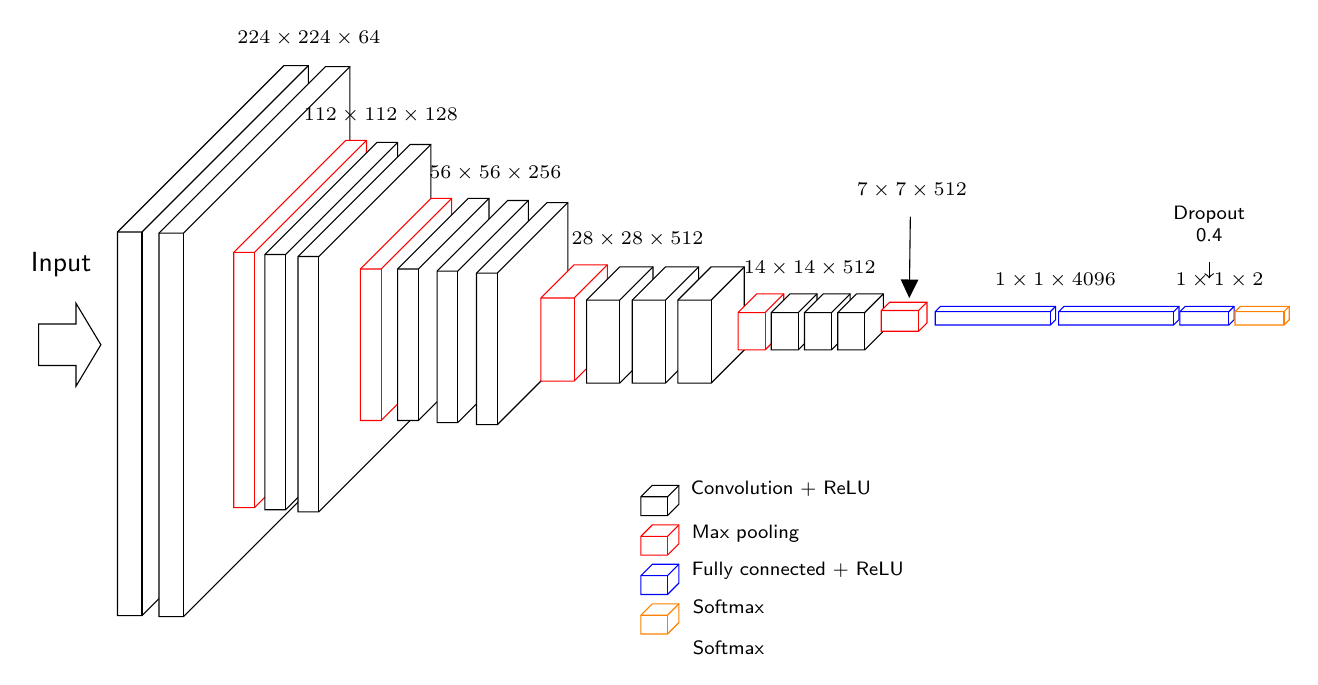
\begin{tikzpicture}[x=0.75pt,y=0.75pt,yscale=-1,xscale=1]

% Conv1-1 
\draw  [fill=white  ,fill opacity=1 ] (44,95.69) -- (124.19,15.5) -- (136,15.5) -- (136,200.31) -- (55.81,280.5) -- (44,280.5) -- cycle ; \draw   (136,15.5) -- (55.81,95.69) -- (44,95.69) ; \draw   (55.81,95.69) -- (55.81,280.5) ;
% Conv 1-2
\draw  [fill=white  ,fill opacity=1 ] (64,96.19) -- (144.19,16) -- (156,16) -- (156,200.81) -- (75.81,281) -- (64,281) -- cycle ; \draw   (156,16) -- (75.81,96.19) -- (64,96.19) ; \draw   (75.81,96.19) -- (75.81,281) ;
% Pooling 1
\draw  [color=red  ,draw opacity=1 ][fill=white  ,fill opacity=1 ] (100,105.5) -- (154,51.5) -- (164,51.5) -- (164,174.5) -- (110,228.5) -- (100,228.5) -- cycle ; \draw  [color=red  ,draw opacity=1 ] (164,51.5) -- (110,105.5) -- (100,105.5) ; \draw  [color=red  ,draw opacity=1 ] (110,105.5) -- (110,228.5) ;
% Conv 2-1
\draw  [fill=white  ,fill opacity=1 ] (115,106.5) -- (169,52.5) -- (179,52.5) -- (179,175.5) -- (125,229.5) -- (115,229.5) -- cycle ; \draw  [color={rgb, 255:red, 0; green, 0; blue, 0 }  ,draw opacity=1 ] (179,52.5) -- (125,106.5) -- (115,106.5) ; \draw  [color={rgb, 255:red, 0; green, 0; blue, 0 }  ,draw opacity=1 ] (125,106.5) -- (125,229.5) ;
% Conv 2-2
\draw  [fill=white  ,fill opacity=1 ] (131,107.5) -- (185,53.5) -- (195,53.5) -- (195,176.5) -- (141,230.5) -- (131,230.5) -- cycle ; \draw  [color={rgb, 255:red, 0; green, 0; blue, 0 }  ,draw opacity=1 ] (195,53.5) -- (141,107.5) -- (131,107.5) ; \draw  [color={rgb, 255:red, 0; green, 0; blue, 0 }  ,draw opacity=1 ] (141,107.5) -- (141,230.5) ;
% Pooling 2
\draw  [color=red  ,draw opacity=1 ][fill=white  ,fill opacity=1 ] (161,113.5) -- (195,79.5) -- (205,79.5) -- (205,152.5) -- (171,186.5) -- (161,186.5) -- cycle ; \draw  [color=red  ,draw opacity=1 ] (205,79.5) -- (171,113.5) -- (161,113.5) ; \draw  [color=red  ,draw opacity=1 ] (171,113.5) -- (171,186.5) ;
% Conv 3-1
\draw  [fill=white  ,fill opacity=1 ] (179,113.5) -- (213,79.5) -- (223,79.5) -- (223,152.5) -- (189,186.5) -- (179,186.5) -- cycle ; \draw  [color={rgb, 255:red, 0; green, 0; blue, 0 }  ,draw opacity=1 ] (223,79.5) -- (189,113.5) -- (179,113.5) ; \draw  [color={rgb, 255:red, 0; green, 0; blue, 0 }  ,draw opacity=1 ] (189,113.5) -- (189,186.5) ;
% Conv 3-2
\draw  [fill=white  ,fill opacity=1 ] (198,114.5) -- (232,80.5) -- (242,80.5) -- (242,153.5) -- (208,187.5) -- (198,187.5) -- cycle ; \draw  [color={rgb, 255:red, 0; green, 0; blue, 0 }  ,draw opacity=1 ] (242,80.5) -- (208,114.5) -- (198,114.5) ; \draw  [color={rgb, 255:red, 0; green, 0; blue, 0 }  ,draw opacity=1 ] (208,114.5) -- (208,187.5) ;
% Conv 3-3
\draw  [fill=white  ,fill opacity=1 ] (217,115.5) -- (251,81.5) -- (261,81.5) -- (261,154.5) -- (227,188.5) -- (217,188.5) -- cycle ; \draw  [color={rgb, 255:red, 0; green, 0; blue, 0 }  ,draw opacity=1 ] (261,81.5) -- (227,115.5) -- (217,115.5) ; \draw  [color={rgb, 255:red, 0; green, 0; blue, 0 }  ,draw opacity=1 ] (227,115.5) -- (227,188.5) ;
% Pooling 3
\draw  [color=red  ,draw opacity=1 ][fill=white  ,fill opacity=1 ] (248,127.5) -- (264,111.5) -- (280,111.5) -- (280,151.5) -- (264,167.5) -- (248,167.5) -- cycle ; \draw  [color=red  ,draw opacity=1 ] (280,111.5) -- (264,127.5) -- (248,127.5) ; \draw  [color=red  ,draw opacity=1 ] (264,127.5) -- (264,167.5) ;
% Conv 4-1
\draw  [fill=white  ,fill opacity=1 ] (270,128.5) -- (286,112.5) -- (302,112.5) -- (302,152.5) -- (286,168.5) -- (270,168.5) -- cycle ; \draw  [color={rgb, 255:red, 0; green, 0; blue, 0 }  ,draw opacity=1 ] (302,112.5) -- (286,128.5) -- (270,128.5) ; \draw  [color={rgb, 255:red, 0; green, 0; blue, 0 }  ,draw opacity=1 ] (286,128.5) -- (286,168.5) ;
% Conv 4-2
\draw  [fill=white  ,fill opacity=1 ] (292,128.5) -- (308,112.5) -- (324,112.5) -- (324,152.5) -- (308,168.5) -- (292,168.5) -- cycle ; \draw  [color={rgb, 255:red, 0; green, 0; blue, 0 }  ,draw opacity=1 ] (324,112.5) -- (308,128.5) -- (292,128.5) ; \draw  [color={rgb, 255:red, 0; green, 0; blue, 0 }  ,draw opacity=1 ] (308,128.5) -- (308,168.5) ;
% Conv 4-3
\draw  [fill=white  ,fill opacity=1 ] (314,128.5) -- (330,112.5) -- (346,112.5) -- (346,152.5) -- (330,168.5) -- (314,168.5) -- cycle ; \draw  [color={rgb, 255:red, 0; green, 0; blue, 0 }  ,draw opacity=1 ] (346,112.5) -- (330,128.5) -- (314,128.5) ; \draw  [color={rgb, 255:red, 0; green, 0; blue, 0 }  ,draw opacity=1 ] (330,128.5) -- (330,168.5) ;
% pooling 4
\draw  [color=red  ,draw opacity=1 ][fill=white  ,fill opacity=1 ] (343,134.5) -- (352,125.5) -- (365,125.5) -- (365,143.5) -- (356,152.5) -- (343,152.5) -- cycle ; \draw  [color={rgb, 255:red, 251; green, 0; blue, 0 }  ,draw opacity=1 ] (365,125.5) -- (356,134.5) -- (343,134.5) ; \draw  [color={rgb, 255:red, 251; green, 0; blue, 0 }  ,draw opacity=1 ] (356,134.5) -- (356,152.5) ;
% Conv 5-1
\draw  [fill=white  ,fill opacity=1 ] (359,134.5) -- (368,125.5) -- (381,125.5) -- (381,143.5) -- (372,152.5) -- (359,152.5) -- cycle ; \draw  [color={rgb, 255:red, 0; green, 0; blue, 0 }  ,draw opacity=1 ] (381,125.5) -- (372,134.5) -- (359,134.5) ; \draw  [color={rgb, 255:red, 0; green, 0; blue, 0 }  ,draw opacity=1 ] (372,134.5) -- (372,152.5) ;
% Conv 5-2
\draw  [fill=white  ,fill opacity=1 ] (375,134.5) -- (384,125.5) -- (397,125.5) -- (397,143.5) -- (388,152.5) -- (375,152.5) -- cycle ; \draw  [color={rgb, 255:red, 0; green, 0; blue, 0 }  ,draw opacity=1 ] (397,125.5) -- (388,134.5) -- (375,134.5) ; \draw  [color={rgb, 255:red, 0; green, 0; blue, 0 }  ,draw opacity=1 ] (388,134.5) -- (388,152.5) ;
% COnv 5-3
\draw  [fill=white  ,fill opacity=1 ] (391,134.5) -- (400,125.5) -- (413,125.5) -- (413,143.5) -- (404,152.5) -- (391,152.5) -- cycle ; \draw  [color={rgb, 255:red, 0; green, 0; blue, 0 }  ,draw opacity=1 ] (413,125.5) -- (404,134.5) -- (391,134.5) ; \draw  [color={rgb, 255:red, 0; green, 0; blue, 0 }  ,draw opacity=1 ] (404,134.5) -- (404,152.5) ;
% Pooling 5
\draw  [color=red  ,draw opacity=1 ][fill=white  ,fill opacity=1 ] (412,133.5) -- (416,129.5) -- (434,129.5) -- (434,139.5) -- (430,143.5) -- (412,143.5) -- cycle ; \draw  [color=red  ,draw opacity=1 ] (434,129.5) -- (430,133.5) -- (412,133.5) ; \draw  [color=red  ,draw opacity=1 ] (430,133.5) -- (430,143.5) ;
% dense 1
\draw  [color=blue  ,draw opacity=1 ][fill=white  ,fill opacity=1 ] (438,134.07) -- (440.57,131.5) -- (496,131.5) -- (496,137.93) -- (493.43,140.5) -- (438,140.5) -- cycle ; \draw  [color=blue  ,draw opacity=1 ] (496,131.5) -- (493.43,134.07) -- (438,134.07) ; \draw  [color=blue  ,draw opacity=1 ] (493.43,134.07) -- (493.43,140.5) ;
% dense 2
\draw  [color=blue  ,draw opacity=1 ][fill=white  ,fill opacity=1 ] (497.43,134.07) -- (500,131.5) -- (555.43,131.5) -- (555.43,137.93) -- (552.86,140.5) -- (497.43,140.5) -- cycle ; \draw  [color=blue  ,draw opacity=1 ] (555.43,131.5) -- (552.86,134.07) -- (497.43,134.07) ; \draw  [color=blue  ,draw opacity=1 ] (552.86,134.07) -- (552.86,140.5) ;
% dense 3
\draw  [color=blue  ,draw opacity=1 ][fill=white  ,fill opacity=1 ] (555.86,134.07) -- (558.43,131.5) -- (582,131.5) -- (582,137.93) -- (579.43,140.5) -- (555.86,140.5) -- cycle ; \draw  [color=blue  ,draw opacity=1 ] (582,131.5) -- (579.43,134.07) -- (555.86,134.07) ; \draw  [color=blue  ,draw opacity=1 ] (579.43,134.07) -- (579.43,140.5) ;
% softmax
\draw  [color=orange  ,draw opacity=1 ][fill=white  ,fill opacity=1 ] (582.43,134.07) -- (585,131.5) -- (608.57,131.5) -- (608.57,137.93) -- (606,140.5) -- (582.43,140.5) -- cycle ; \draw  [color=orange  ,draw opacity=1 ] (608.57,131.5) -- (606,134.07) -- (582.43,134.07) ; \draw  [color=orange  ,draw opacity=1 ] (606,134.07) -- (606,140.5) ;
% input
\draw   (6,140) -- (24,140) -- (24,130) -- (36,150) -- (24,170) -- (24,160) -- (6,160) -- cycle ;
% arrow
\draw    (426,88.25) -- (425.54,124.5) ;
\draw [shift={(425.5,127.5)}, rotate = 270.73] [fill={rgb, 255:red, 0; green, 0; blue, 0 }  ][line width=0.08]  [draw opacity=0] (8.93,-4.29) -- (0,0) -- (8.93,4.29) -- cycle    ;
% conv
\draw  [fill=white  ,fill opacity=1 ] (296.19,223.25) -- (301.69,217.75) -- (314.5,217.75) -- (314.5,226.81) -- (309,232.31) -- (296.19,232.31) -- cycle ; \draw   (314.5,217.75) -- (309,223.25) -- (296.19,223.25) ; \draw   (309,223.25) -- (309,232.31) ;
% max pool
\draw  [color=red  ,draw opacity=1 ][fill=white  ,fill opacity=1 ] (296.19,242.31) -- (301.69,236.81) -- (314.5,236.81) -- (314.5,245.87) -- (309,251.37) -- (296.19,251.37) -- cycle ; \draw  [color=red  ,draw opacity=1 ] (314.5,236.81) -- (309,242.31) -- (296.19,242.31) ; \draw  [color=red  ,draw opacity=1 ] (309,242.31) -- (309,251.37) ;
% fully connected
\draw  [color=blue  ,draw opacity=1 ][fill=white  ,fill opacity=1 ] (296.19,261.25) -- (301.69,255.75) -- (314.5,255.75) -- (314.5,264.81) -- (309,270.31) -- (296.19,270.31) -- cycle ; \draw  [color=blue  ,draw opacity=1 ] (314.5,255.75) -- (309,261.25) -- (296.19,261.25) ; \draw  [color=blue  ,draw opacity=1 ] (309,261.25) -- (309,270.31) ;
% softmax
\draw  [color=orange  ,draw opacity=1 ][fill=white  ,fill opacity=1 ] (296.19,280.31) -- (301.69,274.81) -- (314.5,274.81) -- (314.5,283.87) -- (309,289.37) -- (296.19,289.37) -- cycle ; \draw  [color=orange  ,draw opacity=1 ] (314.5,274.81) -- (309,280.31) -- (296.19,280.31) ; \draw  [color=orange  ,draw opacity=1 ] (309,280.31) -- (309,289.37) ;

 
\draw (1,104) node [anchor=north west][inner sep=0.75pt]   [align=left] {Input};
 
\draw (100.5,-2.5) node [anchor=north west][inner sep=0.75pt]  [font=\scriptsize]  {$224\times 224\times 64$};
 
\draw (132.5,34.5) node [anchor=north west][inner sep=0.75pt]  [font=\scriptsize]  {$112\times 112\times 128$};
 
\draw (261.5,94.5) node [anchor=north west][inner sep=0.75pt]  [font=\scriptsize]  {$28\times 28\times 512$};
 
\draw (344.5,108.5) node [anchor=north west][inner sep=0.75pt]  [font=\scriptsize]  {$14\times 14\times 512$};
 
\draw (193,62.5) node [anchor=north west][inner sep=0.75pt]  [font=\scriptsize]  {$56\times 56\times 256$};

\draw (399,71) node [anchor=north west][inner sep=0.75pt]  [font=\scriptsize]  {$7\times 7\times 512$};

\draw (465.5,114) node [anchor=north west][inner sep=0.75pt]  [font=\scriptsize]  {$1\times 1\times 4096$};

\draw (552.5,114) node [anchor=north west][inner sep=0.75pt]  [font=\scriptsize]  {$1\times 1\times 2$};


\draw (319,214.5) node [anchor=north west][inner sep=0.75pt]  [font=\scriptsize] [align=left] {Convolution + ReLU};

\draw (319.5,235.5) node [anchor=north west][inner sep=0.75pt]  [font=\scriptsize] [align=left] {Max pooling};

\draw (319.5,253.5) node [anchor=north west][inner sep=0.75pt]  [font=\scriptsize] [align=left] {Fully connected + ReLU};

\draw (320,271.5) node [anchor=north west][inner sep=0.75pt]  [font=\scriptsize] [align=left] {Softmax};

\draw (320,291.5) node [anchor=north west][inner sep=0.75pt]  [font=\scriptsize] [align=left] {Softmax};

% Dropout label with arrow
\draw [->] (570,110) -- (570,118);
\draw (570,105) node [anchor=south] [font=\scriptsize] [align=center] {Dropout\\0.4};

\end{tikzpicture}


% \begin{algorithm}
%     \caption{VGG16Modified Architecture}
%     \begin{algorithmic}[1]
%     \Function{VGG16Modified}{}
%         \State Load pre-trained VGG-16 with ImageNet weights
%         \State Extract number of features from final layer: $num\_ftrs \gets$ VGG.classifier[6].in\_features
%         \State Replace final classifier layer with:
%             \State Dropout(p=0.4)
%             \State Linear($num\_ftrs \to 2$) \Comment{Binary classification}
%     \EndFunction
    
%     \Function{Forward}{$x$}
%         \State \Return VGG($x$)
%     \EndFunction
%     \end{algorithmic}
%     \end{algorithm}

\subsubsection{Theoretical Foundation}

VGG-16 is a convolutional neural network architecture developed by Simonyan and Zisserman (2014) at the Visual Geometry Group (VGG) at Oxford, consisting of 16 weight layers including 13 convolutional layers followed by 3 fully connected layers. The architecture is characterized by its simplicity and depth, using small 3×3 convolutional filters stacked in increasing depth, followed by max pooling layers. With approximately 138 million parameters, VGG-16 provides a strong foundation for feature extraction in computer vision tasks.

The primary advantage of employing VGG-16 for transfer learning in fine-grained classification tasks is its hierarchical feature representation capability, which enables the capture of both low-level features (edges, textures) and high-level semantic features. Pre-trained on the ImageNet dataset containing over 1.2 million images across 1,000 classes, VGG-16 offers robust initialization weights that facilitate effective knowledge transfer to domain-specific tasks with limited training data.

VGG-16 has demonstrated superior performance in fine-grained classification tasks compared to conventional techniques. Recent studies show that VGG-16 with logistic regression achieved 97.14\% accuracy on specialized datasets like Leaf12, significantly outperforming traditional approaches that combined color channel statistics, texture features, and classic classifiers which only reached 82.38\% accuracy \citep{pearline2019study}. For our specific task of gull species classification, the hierarchical feature representation capabilities of VGG-16 proved particularly effective at capturing the subtle differences in wing patterns and morphological features that distinguish between the target species.

\subsubsection{Model Adaptation for Fine-Grained Classification}

For our specific fine-grained binary classification task with limited data and class imbalance, the VGG-16 architecture was adapted through a targeted modification strategy:

\begin{itemize}
    \item The pre-trained VGG-16 model was loaded with ImageNet weights.
    \item The feature extraction layers (convolutional base) were preserved to maintain the rich hierarchical representations learned from ImageNet.
    \item The original 1000-class classifier was replaced with a custom binary classification head consisting of: 
    \begin{itemize}
        \item A dropout layer with a rate of 0.4 to reduce overfitting.
        \item A fully-connected layer mapping from the original 4096 features to 2 output classes.
    \end{itemize}
\end{itemize}


% GOOD FOR ALL THE VALUES LIKE OPTIMISER ETC https://ieeexplore.ieee.org/stamp/stamp.jsp?tp=&arnumber=10533638&tag=&tag=1

\citep{zhang2019bird} demonstrated that VGG-16 achieves 94.3\% accuracy on CUB-200-2011 by fine-tuning only the final three layers, a strategy mirrored in my VGG implementation where the classifier head was replaced while preserving ImageNet-initialized convolutional weights.
This approach aligns with successful methodologies in avian species classification using VGG-16 as demonstrated by Brown et al. (2018), where fine-tuning the architecture by modifying the final classification layer enabled the model to retain general feature recognition capabilities while adapting to species-specific visual characteristics \citep{10533638}.

\subsection{Vision Transformer (ViT) Architecture}

\begin{figure}[h]
    \centering
    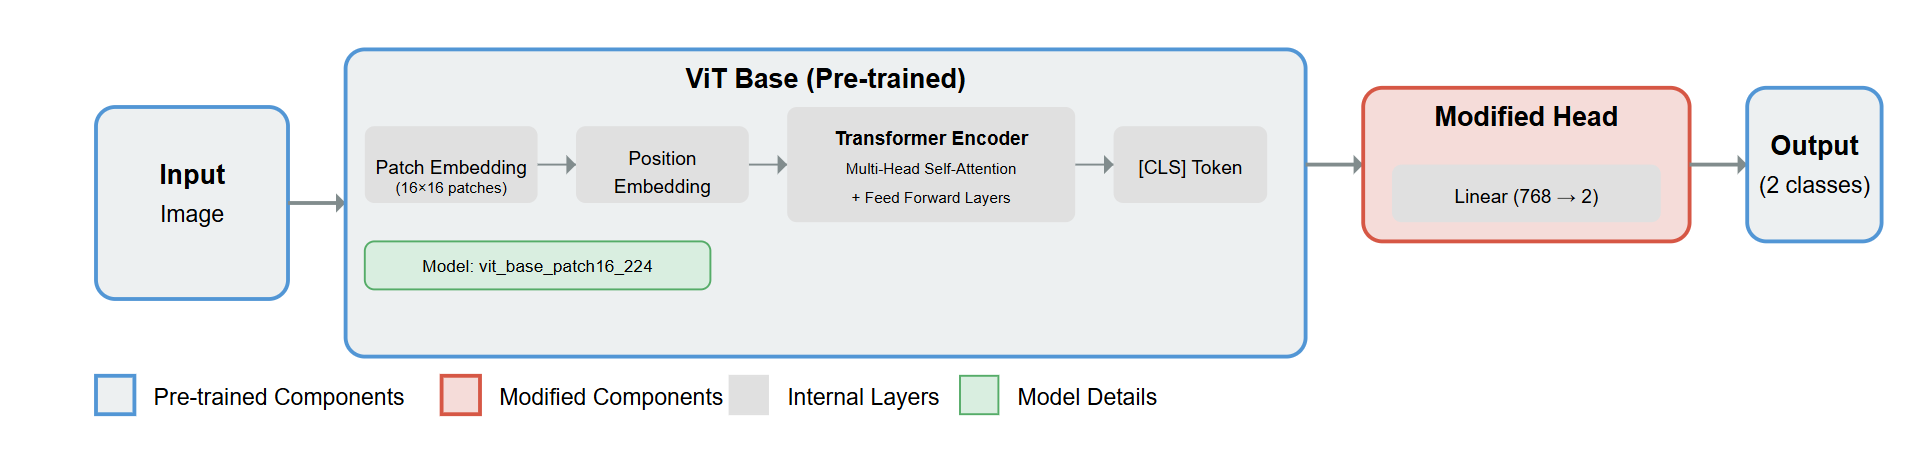
\includegraphics[width=0.8\textwidth]{images/architecture/vit.png}
    \caption{Architecture of the Vision Transformer (ViT) model}
    \label{fig:vit_architecture}
\end{figure}

\subsection{ViT for Fine-Grained Classification}

Vision Transformers (ViT) have emerged as powerful alternatives to convolutional neural networks for visual recognition tasks. First introduced by Dosovitskiy et al. \citep{dosovitskiy2021imageworth16x16words}, ViTs process images as sequences of fixed-size patches, applying transformer-based self-attention mechanisms to model global relationships between image regions. This architecture enables the capture of long-range dependencies within images, making it particularly suitable for fine-grained classification tasks where subtle distinctions between similar classes may depend on relationships between distant image features.

\subsubsection{Vision Transformer Implementation}

For our primary approach, a Vision Transformer using transfer learning from a pre-trained model was implemented:

\begin{itemize}
    \item Base architecture: 'vit\_base\_patch16\_224' pre-trained on ImageNet from the TIMM library \citep{rwightman2021pytorch}
    \item Input resolution: 224×224 pixels with 16×16 pixel patches
    \item Feature dimension: 768-dimensional embeddings
    \item Adaptation strategy: Replacement of the classification head with a binary classifier while preserving the pre-trained transformer blocks
\end{itemize}

The model architecture preserves the core self-attention mechanism of ViT while adapting the final classification layer for our specific binary classification task. This approach follows established transfer learning principles for vision transformers \citep{touvron2021trainingdataefficientimagetransformers}, leveraging representations learned from large-scale datasets to overcome our limited training data constraints.

\subsubsection{Alternative ViT Implementations}

In addition to our primary implementation, we explored two attention-enhanced architectures:

\paragraph{InterpretableViT}
We developed an InterpretableViT model that incorporates explicit attention mechanisms for improved focus on discriminative features:

\begin{itemize}
    \item Separates the class token from patch tokens
    \item Applies a learned attention layer to generate importance weights for each patch
    \item Combines the class token with attention-weighted patch representations
    \item Employs a multi-layer classifier with dropout regularization
\end{itemize}

A key advantage of this architecture is its compatibility with gradient-based visualization techniques. By separating the class token from patch tokens and implementing an explicit attention mechanism, the model facilitates more effective application of Grad-CAM \citep{Selvaraju_2019}, allowing for visualization of discriminative image regions contributing to classification decisions.

% check above referencea and cite as Selvaraju_2019

\paragraph{EnhancedViT}
We also implemented an EnhancedViT that applies attention-based weighting across all tokens:

\begin{itemize}
    \item Processes all tokens (including class token) through an attention mechanism
    \item Generates a single attention-weighted feature representation
    \item Utilizes a specialized classification head with dropout for regularization
\end{itemize}

This implementation draws from research on token aggregation strategies in vision transformers (\href{https://arxiv.org/abs/2012.09688}{Wang et al., 2021}), which shows that attention-weighted token aggregation can improve performance in data-limited regimes.

% https://arxiv.org/pdf/2006.03677 TODO CHECK REF ABOVE
\subsection{Inception v3 Architecture}

\begin{figure}[h]
    \centering
    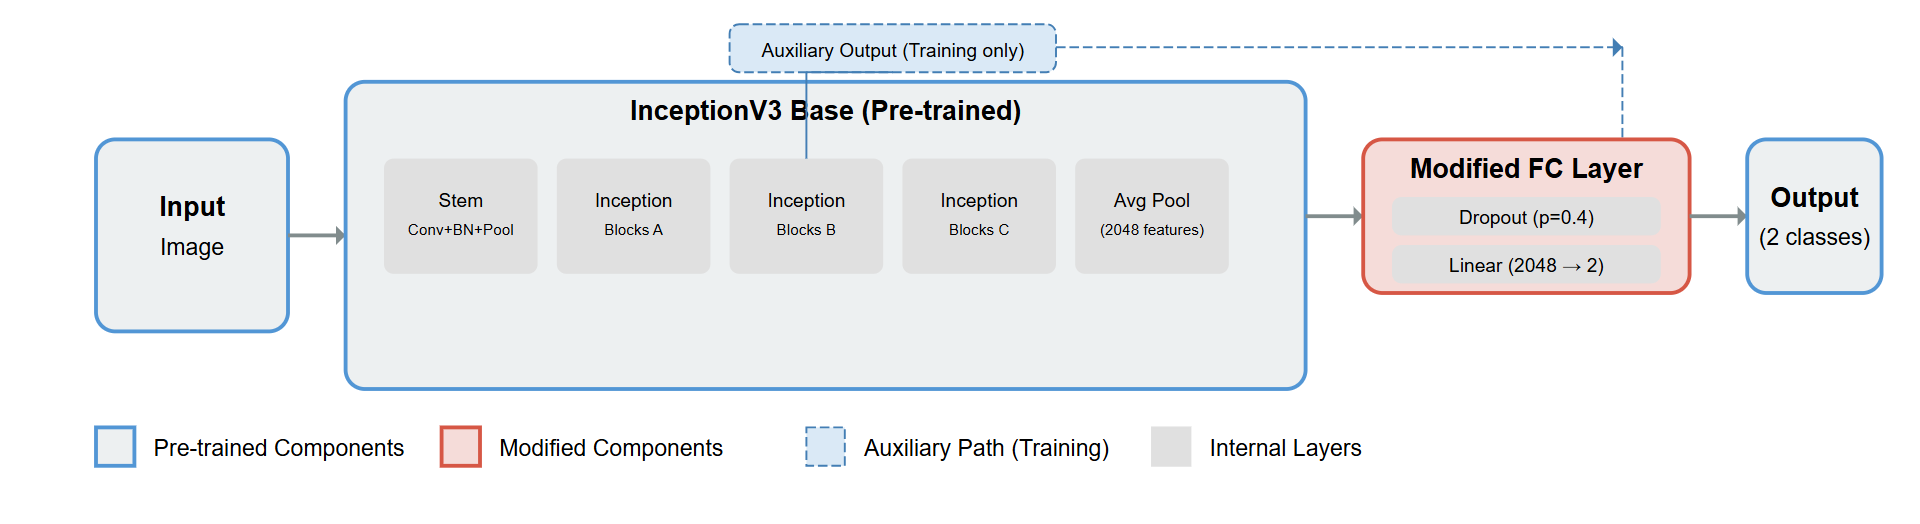
\includegraphics[width=0.8\textwidth]{images/architecture/inception.png}
    \caption{Architecture of the Inception v3 model}
    \label{fig:inception_architecture}
\end{figure}

\subsection*{Theoretical Background}

Inception v3, developed by Szegedy et al. (2016), represents a sophisticated CNN architecture designed to efficiently capture multi-scale features through parallel convolution pathways with varied kernel sizes. The key innovation in Inception architectures is the utilization of \textit{Inception modules} that process the same input tensor through multiple convolutional paths with different receptive fields, and then concatenate the results. This enables the network to capture both fine-grained local patterns and broader contextual information simultaneously \citep{szegedy2015rethinkinginceptionarchitecturecomputer}.

Inception v3 builds upon earlier versions with several important architectural improvements:
\begin{itemize}
    \item Factorized convolutions to reduce computational complexity
    \item Spatial factorization into asymmetric convolutions (e.g., $1 \times n$ followed by $n \times 1$)
    \item Auxiliary classifiers that inject additional gradient signals during training
    \item Batch normalization for improved training stability and faster convergence
    \item Label smoothing regularization to prevent overconfidence
\end{itemize}

These design elements collectively enable Inception v3 to achieve high accuracy while maintaining computational efficiency. Inception architectures are particularly effective for tasks requiring multi-scale feature extraction, such as discriminating between visually similar biological specimens.

\subsubsection{Model-Specific Implementation Details}

Our implementation adapted the pre-trained Inception v3 model for fine-grained gull species classification with the following specific elements:

\begin{itemize}
    \item \textbf{Input Resolution:} Resize operations were performed to $299\times299$ pixels (the standard input size for Inception v3). The larger input resolution ($299\times299$ vs $224\times224$ used by VGG16) provides the Inception architecture with more detailed information, potentially beneficial for capturing the subtle wing pattern differences between gull species.
    
    \item \textbf{Auxiliary Outputs:} A distinctive aspect of our Inception v3 implementation was the utilization of auxiliary outputs during training. Inception v3's auxiliary classifier, which branches off from an intermediate layer, provides an additional gradient path during backpropagation. This helps combat the vanishing gradient problem and provides regularization with auxiliary loss weight of 0.3.
    % (\href{https://arxiv.org/abs/1902.04103}{He et al., 2019})

    \item \textbf{Mixed-Precision Training:} We employed PyTorch's Automatic Mixed Precision (AMP) to accelerate computation while maintaining numerical stability \citep{micikevicius2018mixed}. This technique allows the use of float16 precision where appropriate, which reduces memory usage and increases computational speed, especially beneficial when training on GPU-constrained environments like Google Colab.
\end{itemize}

\subsection{Residual Network (ResNet-50) Implementation}

\begin{figure}[h]
    \centering
    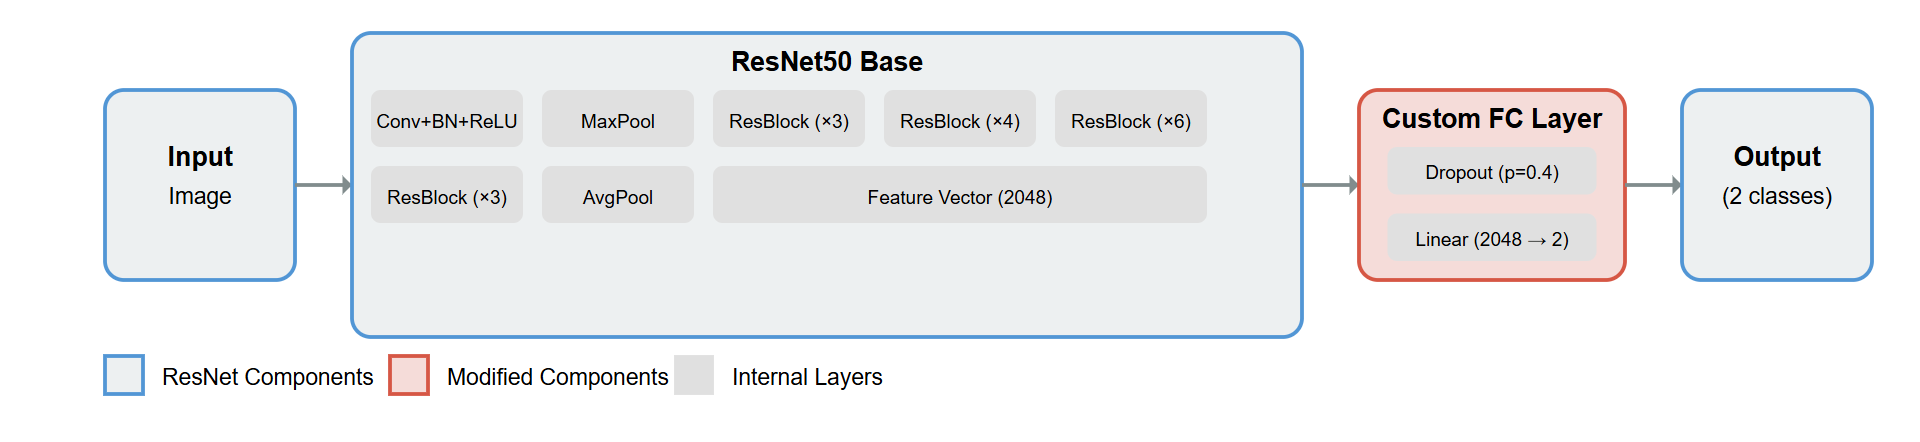
\includegraphics[width=0.8\textwidth]{images/architecture/resnet.png}
    \caption{Architecture of the ResNet-50 model}
    \label{fig:resnet_architecture}
\end{figure}

\subsubsection{Architecture-Specific Enhancements}

A distinctive aspect of our ResNet-50 implementation was the incorporation of image sharpening as a preprocessing technique. We applied a 3×3 Laplacian sharpening kernel to enhance edge definition and accentuate the subtle diagnostic features crucial for distinguishing between gull species. This approach was inspired by research showing that edge enhancement can improve the detection of fine-grained morphological features in avian classification tasks {\href{https://openaccess.thecvf.com/content_cvpr_2014/papers/Berg_Birdsnap_Large-scale_Fine-grained_2014_CVPR_paper.pdf}{Berg et al., 2014}}.

The sharpening kernel was systematically applied to both training and evaluation pipelines using OpenCV's filter2D function, ensuring consistent feature enhancement across all dataset partitions. This preprocessing step proved particularly valuable for highlighting distinctive wingtip patterns and subtle plumage characteristics that serve as key discriminative features between the target species.

\subsection{Custom CNN with Squeeze-and-Excitation Blocks}

\begin{figure}[h]
    \centering
    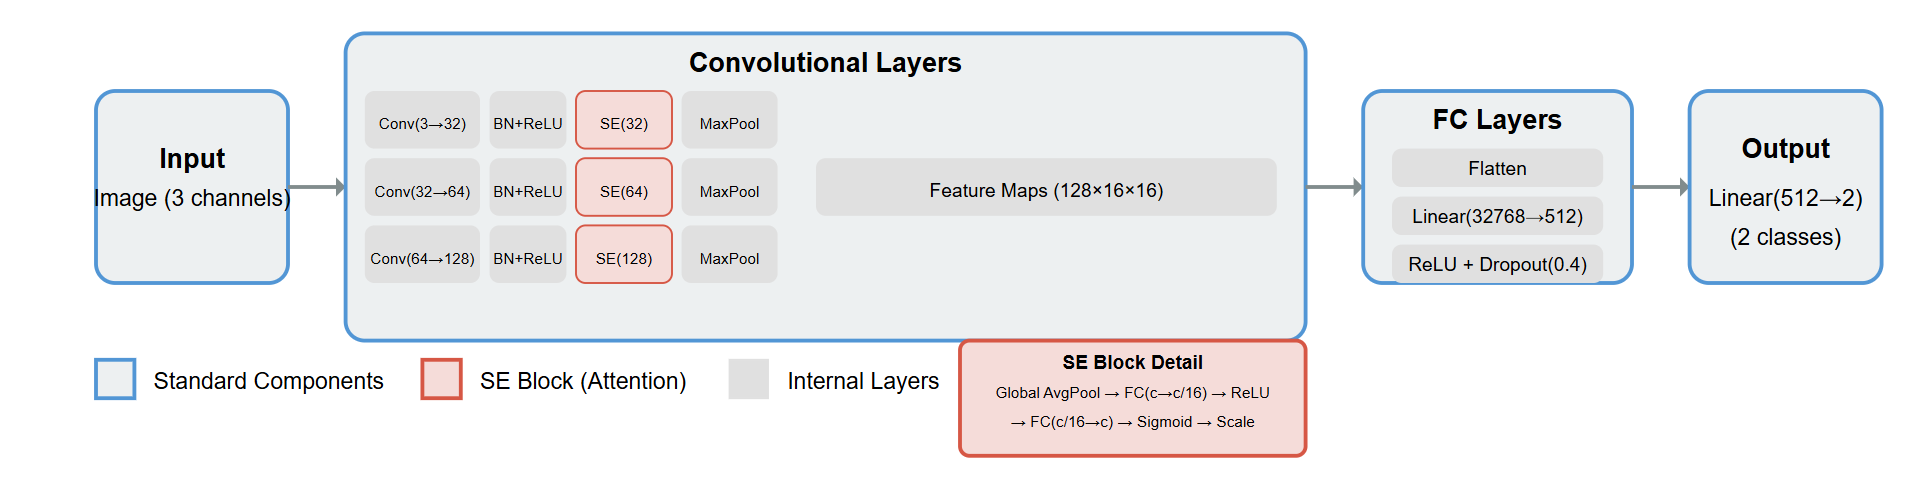
\includegraphics[width=0.8\textwidth]{images/architecture/improvedcnn.png}
    \caption{Architecture of the Custom CNN with Squeeze-and-Excitation Blocks}
    \label{fig:improvedcnn_architecture}
\end{figure}

\subsubsection{Architectural Design}

To address the challenges of limited data and class imbalance in fine-grained classification, we developed a lightweight custom CNN architecture incorporating attention mechanisms. Our approach employs Squeeze-and-Excitation (SE) blocks, which enhance feature representation by modeling channel interdependencies through an attention mechanism. The SE block, as introduced by Hu et al. \citep{Hu_2018_CVPR}, adaptively recalibrates channel-wise feature responses to emphasize informative features while suppressing less useful ones.

The architecture consists of three convolutional blocks, each followed by batch normalization, ReLU activation, and an SE block. The SE block performs two key operations:
\begin{itemize}
    \item \textbf{Squeeze}: Global average pooling across spatial dimensions to generate channel-wise statistics
    \item \textbf{Excitation}: A fully connected layer that produces modulation weights for each channel
\end{itemize}

This channel-wise attention mechanism has been shown to improve model performance with minimal computational overhead \citep{Hu_2018_CVPR}. The SE blocks in our implementation use a reduction ratio of 16, balancing parameter efficiency and representational power.

\subsubsection{Custom CNN-Specific Training Approach}

Unlike the transfer learning approaches used with pre-trained models, our custom CNN was trained from scratch with some specific optimization strategies:

\begin{itemize}
    \item \textbf{Cosine Annealing scheduler}: Our learning rate schedule follows a cosine annealing pattern with a period of 20 epochs, allowing the learning rate to oscillate and potentially escape local minima.
    
% IRRELEVANT (\href{https://arxiv.org/abs/1608.03983}{Loshchilov and Hutter, 2017})
    
    \item \textbf{Specialized augmentation}: The custom CNN particularly benefited from more aggressive data augmentation strategies to compensate for the lack of pre-trained weights, including stronger rotations and more extensive color jittering than used with the transfer learning models.
\end{itemize}

\section{Model Interpretability Methodologies}

Deep learning models, particularly Convolutional Neural Networks (CNNs) and Vision Transformers (ViTs), are often criticized for their lack of transparency, functioning as "black boxes" wherein the decision-making process remains opaque to human observers. For critical applications like wildlife species classification, understanding how these models arrive at their predictions is essential for establishing trust and validating results \citep{Selvaraju_2019}. This section outlines the methodologies implemented to visualize and interpret the classification decisions of both the CNN architecture and Vision Transformer (ViT) models used in this study.

\subsection{Gradient-weighted Class Activation Mapping (Grad-CAM)}

Gradient-weighted Class Activation Mapping (Grad-CAM) is a widely adopted visualization technique that produces visual explanations for decisions made by CNN-based models without requiring architectural changes or retraining \citep{Selvaraju_2019}. It generates coarse localization maps highlighting the regions in the input image that significantly influenced the model's prediction for a specific class.

\subsubsection{Theoretical Foundation}

Grad-CAM extends the Class Activation Mapping (CAM) approach \citep{zhou2015learningdeepfeaturesdiscriminative} by utilizing the gradient information flowing into the final convolutional layer of a CNN. Unlike CAM, which requires modifications to the network architecture and retraining, Grad-CAM can be applied to any CNN-based architecture without architectural changes, making it more versatile.

The fundamental principle behind Grad-CAM is that the final convolutional layer in a CNN retains spatial information while encoding high-level semantics. By analyzing how the gradients of a specific class score flow into this layer, Grad-CAM can identify the regions in the input image that are most influential for the prediction.

% \begin{algorithm}
% \caption{Gradient-weighted Class Activation Mapping (Grad-CAM)}
% \begin{algorithmic}[1]
% \Input Input image $I$, CNN model $f$, target class $c$, final convolutional layer feature maps $A^k$
% \Output Heatmap $L_{Grad-CAM}^c$
% \State Perform forward pass on model $f$ with input image $I$ to obtain prediction score $y^c$
% \State Compute gradients of score $y^c$ with respect to feature maps $A^k$: $\frac{\partial y^c}{\partial A^k}$
% \State Apply global average pooling to gradients to obtain importance weights $\alpha_k^c$: 
%        $\alpha_k^c = \frac{1}{Z}\sum_i \sum_j \frac{\partial y^c}{\partial A_{ij}^k}$
% \State Calculate weighted combination of feature maps: 
%        $L_{Grad-CAM}^c = ReLU\left(\sum_k \alpha_k^c A^k\right)$
% \State Normalize $L_{Grad-CAM}^c$ to range [0, 1]
% \State Resize $L_{Grad-CAM}^c$ to input image dimensions
% \Return $L_{Grad-CAM}^c$
% \end{algorithmic}
% \end{algorithm}

The ReLU function is applied to the weighted combination of feature maps to focus only on features that have a positive influence on the class of interest, effectively eliminating features that suppress the class.

\subsubsection{Methodology for CNN models}

In this study, Grad-CAM was implemented for the VGG16 model by targeting the final convolutional layer (features[-1]). The implementation involves several key steps:

\begin{enumerate}
    \item \textbf{Hook Registration}: Forward and backward hooks are registered on the target layer to capture activations during the forward pass and gradients during the backward pass.
    
    \item \textbf{Forward Pass}: The input image is passed through the network to obtain the model's prediction.
    
    \item \textbf{Backpropagation}: The gradient of the score for the target class (either the predicted class or a specified class) with respect to the feature maps of the target layer is computed through backpropagation.
    
    \item \textbf{Global Average Pooling}: These gradients undergo global average pooling to obtain weights indicating the importance of each channel for the target class.
    
    \item \textbf{Weighted Combination}: The weights are applied to the activations of the target layer to create a weighted combination of feature maps.
    
    \item \textbf{ReLU Application}: A ReLU function is applied to the weighted combination to focus only on features that have a positive influence on the class of interest.
    
    \item \textbf{Normalization}: The resulting heatmap is normalized to the range [0, 1] for consistent visualization.
    
    \item \textbf{Visualization}: The heatmap is resized to match the input image dimensions and overlaid on the original image using a colormap (typically 'jet') to highlight regions the model focused on for its prediction.
\end{enumerate}



Similar implementation was implemented for other models: Inceptionv3, ResNet50, and CustomCNN. 

\subsection{Attention Rollout for Vision Transformers}

Vision Transformers process images differently from CNNs, using self-attention mechanisms rather than convolution operations to model relationships between image patches. Therefore, a different approach called Attention Rollout is used to visualize ViT decision-making \citep{abnar2020attention}.

\subsubsection{Theoretical Foundation}

The Attention Rollout method is designed to visualize how information flows through the layers of a Transformer model. In Vision Transformers, the input image is divided into fixed-size patches, and each patch is linearly embedded along with position embeddings. A special classification token ([CLS]) is added, and the sequence of embedded patches is processed through multiple layers of self-attention.

Attention Rollout computes a measure of how the [CLS] token attends to each image patch by propagating attention through all layers of the network. This provides insight into which parts of the image the model considers most relevant for classification.

\subsubsection{Methodology for ViT}

The implementation of Attention Rollout for the ViT model follows these steps:

\begin{enumerate}
    \item \textbf{Attention Map Collection}: Forward hooks are registered on each transformer block to collect attention maps during the forward pass of an input image.
    
    \item \textbf{QKV Processing}: For each attention head, the query (Q), key (K), and value (V) matrices are extracted and processed to compute the raw attention weights between different tokens.
    
    \item \textbf{Head Averaging}: Attention weights from all heads in each layer are averaged to get a single attention map per transformer block.
    
    \item \textbf{Discard Ratio Application}: Optionally, a threshold is applied to filter out low-attention connections, focusing only on the most significant attention patterns.
    
    \item \textbf{Attention Rollout Computation}: Starting with an identity matrix, attention maps from each layer are sequentially multiplied to account for how attention propagates through the entire network.
    
    \item \textbf{CLS Token Attention Extraction}: The attention weights from the classification ([CLS]) token to each image patch are extracted, which indicates the importance of each patch for the final classification.
    
    \item \textbf{Reshaping and Visualization}: These weights are reshaped to match the spatial dimensions of the input image (typically 14×14 for ViT-Base with patch size 16) and then upsampled to create a heatmap that can be overlaid on the original image.
\end{enumerate}

This method provides insights into how the ViT model attends to different parts of an image when making a prediction \citep{chefer2021generic}.

\subsection{Grad-CAM for Vision Transformers}

In addition to Attention Rollout, this study also implements Grad-CAM for Vision Transformers to provide a more direct comparison with the CNN-based visualizations. Two variants of Grad-CAM for ViT were implemented in this study: Enhanced ViT and Interpretable ViT, each with specific architectural modifications to facilitate interpretation.

\subsection{Enhanced ViT Implementation}

The Enhanced ViT approach modifies the standard ViT architecture to facilitate Grad-CAM visualization:

\begin{itemize}
\item \textbf{Model Architecture:} The Enhanced ViT model extends the base ViT by replacing the original head with an identity layer, adding an attention layer to compute scalar importance scores for each token, and implementing a classifier that operates on attention-weighted features.
\item \textbf{Token Feature Registration:} The model registers hooks to capture token features during the forward pass and their gradients during backpropagation.
\item \textbf{Gradient Computation:} When computing Grad-CAM, the class token is excluded, and only the patch tokens are considered.
\item \textbf{Spatial Reshaping:} The tokens and gradients are reshaped to recover the 2D spatial structure ($h \times w$ grid) from the sequence of tokens.
\item \textbf{Grad-CAM Generation:} Similar to traditional Grad-CAM, channel-wise weights are computed from gradients and applied to token features to create the activation map.
\end{itemize}

\subsection{Interpretable ViT Implementation}

The Interpretable ViT variant uses a different approach to extract and utilize token information:

\begin{itemize}
\item \textbf{Dual-Stream Architecture:} This implementation processes the class token and patch tokens separately.
\item \textbf{Attention Weights Calculation:} An explicit attention layer computes importance weights for patch tokens, determining how much each patch contributes to the final representation.
\item \textbf{Feature Combination:} The class token and weighted patch features are concatenated before classification, providing the classifier with both global context (class token) and attention-weighted local features.
\item \textbf{Grad-CAM Calculation:} During Grad-CAM computation, gradients flow through this combined representation, providing a more nuanced view of how different parts of the image contribute to the classification.
\end{itemize}

Both approaches enable visualization of the ViT's decision-making process using gradient information, but with different mechanisms for integrating token features and attention weights.

\subsection{Comparison Framework}

To facilitate a fair comparison between CNN model and ViT interpretability, the following standardized approach was implemented:

\begin{itemize}
\item \textbf{Consistent Processing:} All models process the same test images with identical preprocessing (resizing to $224 \times 224$ and normalization).
\item \textbf{Three-Panel Visualization:} Each result is presented with three panels:
\begin{enumerate}
\item Original image
\item Raw heatmap showing the attention or Grad-CAM output
\item Overlay of the heatmap on the original image
\end{enumerate}
\item \textbf{Classification Analysis:} Both correct and incorrect predictions are analyzed to understand model behavior in different scenarios.
\item \textbf{Visualization Standardization:} Similar color maps (jet) and overlay techniques are used for all methods to maintain visual consistency.
\item \textbf{Quantitative Assessment:} Confusion matrices are generated for all models to quantitatively assess their performance alongside the visual interpretations.
\end{itemize}

By implementing these complementary interpretability techniques, this research provides insights into how different neural network architectures—traditional CNNs and modern Transformers—approach the same classification task and what are the distinguishing features between the two classes. The visualizations reveal different feature priorities and decision strategies that each architecture employs, contributing to a deeper understanding of model behavior \cite{dosovitskiy2021imageworth16x16words}.


% \begin{itemize}
%     \item \textbf{Confidence Calculation}: Computing the softmax probability for the predicted class to indicate the model's confidence.
    
%     \item \textbf{Misclassification Analysis}: For incorrectly classified images, both the original image and Grad-CAM visualization are saved with annotations indicating the true and predicted classes.
    
%     \item \textbf{Three-Panel Visualization}: Creating a standardized visualization with the original image, the Grad-CAM heatmap, and the overlay for easy comparison.
% \end{itemize}



% \subsection{Implementation Details}

% The interpretability frameworks were implemented with the following technical considerations:

% \subsubsection{Grad-CAM for VGG16}
% \begin{itemize}
%     \item \textbf{Target Layer}: The last convolutional layer of VGG16 (features[-1])
%     \item \textbf{Gradient Calculation}: Using PyTorch's autograd functionality for backpropagation
%     \item \textbf{Output Format}: Three-panel visualization with original image, Grad-CAM heatmap, and overlay
%     \item \textbf{Confidence Annotation}: Each visualization includes the model's confidence percentage
%     \item \textbf{Organization}: Images organized by class and correctness of prediction
% \end{itemize}

% \subsubsection{Attention Rollout for ViT}
% \begin{itemize}
%     \item \textbf{Model Type}: Vision Transformer Base model with 16×16 patch size
%     \item \textbf{Attention Collection}: Forward hooks on all self-attention blocks
%     \item \textbf{QKV Extraction}: Capturing query, key, and value matrices for attention computation
%     \item \textbf{Discard Ratio}: Configurable threshold (set to 0.0) to filter out low-attention areas
%     \item \textbf{Rollout Computation}: Sequential multiplication of attention maps across layers
% \end{itemize}

% \subsubsection{Grad-CAM for ViT}
% \begin{itemize}
%     \item \textbf{Model Architecture}: Custom InterpretableViT with token feature extraction
%     \item \textbf{Gradient Hooks}: Custom hooks to capture token features and their gradients
%     \item \textbf{Attention Layer}: Additional attention mechanism to weight patch tokens
%     \item \textbf{Feature Combination}: Concatenation of class token and weighted patch features
%     \item \textbf{Visualization}: Consistent with the VGG16 Grad-CAM approach for comparison
% \end{itemize}

% \appendix
% \section{Additional Interpretability Techniques}
% \label{appendix:add_interpret}

% In addition to the Grad-CAM method discussed in the main sections of this report, several other interpretability techniques were explored during this research. While not featured prominently in the main analysis, these methods offer complementary perspectives on model decision-making.

% \subsection{DeepLIFT}

% DeepLIFT (Deep Learning Important FeaTures) was implemented using the Captum library for the VGG16 and ViT models. This technique compares activations against a reference baseline (typically zeros) to determine feature importance:

% \begin{itemize}
%     \item A zero baseline tensor is created as a reference point
%     \item Attribution scores are calculated comparing actual activations to this baseline
%     \item Channel-wise attributions are aggregated and normalized for visualization
%     \item Color maps are applied to create interpretable heatmaps
% \end{itemize}

% While DeepLIFT provides more theoretically grounded attributions than simple gradient methods, it was not extended to all models due to it not being used as frequently by others as other techniques such as grad cam/
% \subsection{Saliency Maps}

% Basic saliency maps were implemented for both VGG16 and Vision Transformer models:

% \begin{itemize}
%     \item Input tensors are configured to track gradients
%     \item Forward and backward passes compute gradients from prediction to input
%     \item Absolute values of gradients reveal input sensitivity
%     \item Channel-wise maximum operations create single-channel visualizations
% \end{itemize}


% % This paper examines saliency methods, which are explanation techniques designed to highlight relevant features in inputs (particularly images) that influence a machine learning model's predictions. The authors propose a methodology to evaluate whether these explanation methods are actually providing meaningful insights about the model and data. Their key findings include:

% % Many popular saliency methods fail basic "sanity checks" - they produce explanations that are independent of model parameters and training data.
% % The authors propose two randomization tests to evaluate explanation methods:

% % Model parameter randomization test: Compares explanations from a trained model vs. a randomly initialized model
% % Data randomization test: Compares explanations from a model trained on proper data vs. one trained on randomly permuted labels


% % Several widely used methods (Guided BackProp and Guided GradCAM) fail these tests, meaning they can't provide insights about the model or data relationships.
% % Some methods (standard Gradients and GradCAM) pass the tests, suggesting they are more reliable.
% % The authors demonstrate that some saliency methods produce outputs visually similar to simple edge detectors, which require neither training data nor model knowledge.

% % The paper warns that visual assessment alone can be misleading when evaluating explanation methods. Methods that fail their proposed tests are inadequate for tasks like finding data outliers, explaining model relationships, or debugging models. The authors support their findings with theoretical analysis of linear models and simple convolutional neural networks.
% \subsection{Integrated Gradients for Vision Transformers}

% For the Vision Transformer model specifically, Integrated Gradients was implemented using Captum:

% \begin{itemize}
%     \item Path integrals are approximated between baseline and input images
%     \item 50 interpolation steps were used for the approximation
%     \item Attributions are processed to align with spatial image dimensions
%     \item Results are normalized for consistent visualization
% \end{itemize}

% While theoretically sound, Integrated Gradients requires significantly more computation time than Grad-CAM. Additionally, the literature review indicated that Grad-CAM adaptations for Vision Transformers often provide more intuitive visualizations for classification tasks \cite{chefer2021transformer}.

% \subsection{Guided Backpropagation for Vision Transformers}

% Guided Backpropagation was adapted specifically for Vision Transformers:

% \begin{itemize}
%     \item Modified gradient flow during backpropagation highlights positive influences
%     \item Implementation uses Captum's GuidedBackprop with model-specific wrappers
%     \item Results are post-processed to create single-channel visualizations
% \end{itemize}

% This method produces visually cleaner results than standard saliency maps but lacks the localization capabilities of Grad-CAM. Additionally, research has shown that guided backpropagation may highlight input patterns rather than decision-relevant features \cite{nie2018theoretical}.

% \subsection{Conclusion on Additional Methods}

% These additional interpretability techniques were implemented primarily for exploration and comparison. Grad-CAM was selected as the primary visualization method for the main analysis due to its:

% \begin{itemize}
%     \item Widespread adoption in the literature
%     \item Consistent performance across model architectures
%     \item Ability to produce class-discriminative visualizations
%     \item Better localization of discriminative regions
%     \item Lower computational requirements
%     \item Stronger theoretical foundation compared to simple gradient methods
% \end{itemize}

% The implementation details and experimental results for these additional techniques are preserved here to document the comprehensive approach taken toward model interpretability in this research.

% Though straightforward to implement, saliency maps,  guided backpropagation were not highlighted in the main analysis as they can be noisy and lack the class-discriminative properties of Grad-CAM. Additionally, as noted by \cite{Adebayo2018}, simple gradient methods sometimes fail sanity checks that Grad-CAM passes.

% 3. Of the methods tested, Gradients and GradCAM pass the sanity checks, while Guided BackProp and
% Guided GradCAM are invariant to higher layer parameters; hence, fail.
% 4. Consequently, our findings imply that the saliency methods that fail our proposed tests are incapable
% of supporting tasks that require explanations that are faithful to the model or the data generating
% process.  \href{https://arxiv.org/pdf/1810.03292}{(Guided and saliency not good)}

% TODO
% \appendix
\section{Additional Interpretability Techniques}
\label{appendix:add_interpret}

In addition to the Grad-CAM and attention rollout methods discussed in the main sections of this report, several other interpretability techniques were explored during this research.

\subsection{DeepLIFT}

DeepLIFT (Deep Learning Important FeaTures) was implemented using the Captum library for the VGG16 and ViT models. This technique compares activations against a reference baseline (typically zeros) to determine feature importance:

\begin{itemize}
\item A zero baseline tensor is created as a reference point
\item Attribution scores are calculated comparing actual activations to this baseline
\item Channel-wise attributions are aggregated and normalized for visualization
\end{itemize}

While DeepLIFT provides theoretically grounded attributions, it was not adopted for the main analysis due to its limited adoption in the literature compared to prevalent techniques like Grad-CAM.

\subsection{Saliency Maps}

\begin{itemize}
\item Gradients of predictions with respect to input pixels are computed
\item Absolute values of gradients are visualized as sensitivity maps
\end{itemize}

Saliency maps, though computationally efficient, often produce noisy visualizations and lack class-discriminative properties. As shown in prior work \citep{Adebayo2018}, they may also fail basic sanity checks, making them unreliable for tasks requiring faithful explanations.

\subsection{Integrated Gradients for Vision Transformers}

Integrated Gradients was implemented for ViT using 50 interpolation steps:

\begin{itemize}
    \item Path integrals are approximated between baseline and input images
    \item 50 interpolation steps were used for the approximation
    \item Attributions are processed to align with spatial image dimensions
    \item Results are normalized for consistent visualization
\end{itemize}

Despite its theoretical soundness, Integrated Gradients requires significantly more computation than Grad-CAM. Additionally, the literature review indicated that Grad-CAM adaptations for Vision Transformers often provide more intuitive visualizations for classification tasks \cite{chefer2021transformer}

\subsection{Guided Backpropagation for ViT}


\begin{itemize}
    \item Modified gradient flow during backpropagation highlights positive influences
    \item Implementation uses Captum's GuidedBackprop with model-specific wrappers
    \item Results are post-processed to create single-channel visualizations
\end{itemize}

While visually cleaner than saliency maps, Guided Backpropagation has two key limitations: (1) it lacks localization capabilities, and (2) as demonstrated by \citep{Adebayo2018}, it fails parameter randomization tests, (3) it may highlight input patterns rather than model decision logic \cite{nie2018theoretical}.

\subsection{Justification for Grad-CAM}

Grad-CAM was chosen as the primary interpretability method for this study due to its unique advantages over the alternatives:

\begin{itemize}
\item \textbf{Theoretical Robustness}: Grad-CAM passes sanity checks (e.g., parameter randomization tests) that methods like Guided Backpropagation and Guided Grad-CAM fail \citep{Adebayo2018}.
\item \textbf{Class-Discriminative}: Unlike saliency maps or Integrated Gradients, Grad-CAM highlights regions relevant to specific predicted classes.
\item \textbf{Architecture Flexibility}: Works consistently across CNNs (e.g., VGG16, ResNet) and adapted Vision Transformers.
\item \textbf{Computational Efficiency}: Requires only a single backward pass per class, unlike path-based methods (e.g., Integrated Gradients).
\item \textbf{Empirical Validation}: Supported by extensive literature \citep{Selvaraju_2019, chefer2021generic} demonstrating its effectiveness for classification tasks.
\end{itemize}
% Add these to your bibliography
% \bibitem{adebayo2018sanity} Adebayo, J., Gilmer, J., Muelly, M., Goodfellow, I., Hardt, M., \& Kim, B. (2018). Sanity checks for saliency maps. In Advances in Neural Information Processing Systems.
% \bibitem{chefer2021transformer} Chefer, H., Gur, S., \& Wolf, L. (2021). Transformer interpretability beyond attention visualization. In Proceedings of the IEEE/CVF Conference on Computer Vision and Pattern Recognition.
% \bibitem{nie2018theoretical} Nie, W., Zhang, Y., \& Patel, A. (2018). A theoretical explanation for perplexing behaviors of backpropagation-based visualizations. In International Conference on Machine Learning.

\section{Feature Analysis for Fine-Grained Gull Classification}

A multi-stage approach was employed to extract and analyze region-specific features.

\subsection{Image Selection}
From the normalized dataset, 200 high-resolution images (100 per species) were selected based on the following criteria:
\begin{itemize}
\item Correct classification by the best-performing VGG-16 model
\item Prominent Grad-CAM activations in wing or wingtip regions
\item Clear visibility of upperwing or wingtip in the image
\item High resolution image
\end{itemize}

\subsection{Manual Segmentation}
Using Adobe Photoshop, segmentation masks with color-coded regions were created with a specific color for each type of region: wing, wingtip, and head.

\subsection{Normalization}
Applied min-max normalization\citep{monzon_image_normalization} (0-255) to grayscale conversions using OpenCV's \texttt{NORM\_MINMAX}.
This helped standardize intensity values and mitigate the effects of differing lighting conditions ensuring that pixel intensity values were scaled consistently across the dataset, providing a reliable foundation for subsequent region-based analysis.

\subsection{Region Extraction}

Using OpenCV's \texttt{inRange} for color-based thresholding, pixels within $\pm$10 intensity values of each target color were extracted and used for further analysis.

\section{Local Binary Pattern}

Local Binary Patterns (LBP) represents a powerful and computationally efficient approach for texture analysis, first introduced by Ojala et al. \Citep{1017623}. The fundamental principle of LBP is that it characterizes the local spatial structure of an image's texture by comparing each pixel with its neighbors, generating a binary pattern that serves as a texture descriptor. This method offers several key advantages for biological image analysis:

\begin{itemize}
    \item Gray-scale invariance, making it robust to lighting variations
    \item Computational simplicity while maintaining high discriminative power
    \item \textbf{Rotation-invariant abstract features} derived from binary patterns (number of 1s and transitions) rather than raw LBP codes
    \item Robustness to monotonic illumination changes
    \item Ability to capture micro-patterns in texture that may be imperceptible to human observers
\end{itemize}

For our seagull species differentiation task, these properties are particularly valuable as they allow us to analyze subtle texture differences in plumage that may remain consistent across varying lighting conditions and viewing angles.

\subsection{Implementation Methodology}

\subsubsection{LBP Calculation Process}

The core LBP calculation involves several carefully calibrated parameters:

\begin{itemize}
    \item \textbf{Radius (R)}: Set to 3 pixels, defining the distance from the center pixel to its neighbors
    \item \textbf{Number of Points (P)}: Set to $8 \times R$ (24 points), determining the sampling resolution around the circle
    \item \textbf{Method}: Default and Uniform methods were tested. "Default" method produces the full range of LBP codes, preserving all pattern details while the "Uniform" method Focuses on patterns with at most two bitwise transitions from 0 to 1 or vice versa, reducing feature dimensionality while retaining discriminative power.
\end{itemize}

For each region, only pixels within the segmentation mask are considered for LBP calculation. The LBP operation proceeds as follows:

\begin{enumerate}
    \item For each pixel in the selected region of the normalised image, a circular neighborhood of radius R with P sampling points is examined
    \item Each sampling point is compared to the center pixel value
    \item If the sampling point value is greater than or equal to the center pixel value, a '1' is assigned; otherwise, a '0'
    \item The resulting binary pattern is converted to a decimal value, which becomes the LBP code for that pixel
    \item The collection of LBP codes across the entire region is compiled into a normalized histogram to create comparable feature vectors.
\end{enumerate}

\subsubsection{Novel Abstract Pattern Analysis}

A key contribution of our methodology is the extraction of abstract pattern features from the binary LBP codes. This approach was done to prevent the angles of the regions in the image that varied across from causing rotation variance.

\begin{enumerate}
    \item \textbf{Binary Pattern Generation}: Converting each LBP value to its N\_POINTS-bit binary representation
    \item \textbf{Ones Count Analysis}: Counting the number of '1' bits in each pattern, representing the frequency of neighboring pixels brighter than the central pixel
    \begin{itemize}
        \item Higher values indicate more bright spots or edges within darker regions
        \item Lower values suggest more uniform dark or bright regions
    \end{itemize}
    \item \textbf{Transitions Analysis}: Counting the number of 0-to-1 or 1-to-0 transitions in each pattern, capturing the complexity of the texture pattern
    \begin{itemize}
        \item Higher values indicate more complex textures with frequent brightness changes
        \item Lower values suggest smoother textures with fewer brightness changes
    \end{itemize}
    \item \textbf{Histogram Creation}: Compiling the distributions of these abstract features into normalized histograms
\end{enumerate}

From the LBP histograms, several statistical texture features were calculated:

\begin{enumerate}
    \item \textbf{Entropy}: Quantifies the randomness or unpredictability of the texture using Shannon entropy. Higher values indicate more complex textures with greater variability.

    \item \textbf{Uniformity}: Measures the textural uniformity by calculating the sum of squared elements in the histogram. Lower values indicate more heterogeneous textures.

    \item \textbf{Contrast}: Quantifies the intensity difference between a pixel and its neighborhood. Higher values indicate more distinct intensity variations. This calculates a weighted variance where the weights are the histogram probabilities.

    \item \textbf{Homogeneity}: Measures the closeness of the distribution of elements in the histogram. Higher values indicate smoother textures.
\end{enumerate}

These statistical measures provide a comprehensive profile of texture characteristics that can be compared between species.

\subsection{Comparative Analysis Implementation}

To quantify the differences between species, the implementation calculates several distribution similarity metrics:

\begin{enumerate}
    \item \textbf{KL Divergence}: A symmetric version of the Kullback-Leibler divergence that measures how one probability distribution diverges from another

    \item \textbf{Earth Mover's Distance}: Measures the minimum ``work'' required to transform one histogram into another, considering the distance between bins

    \item \textbf{Chi-Square Distance}: A statistical test that measures the difference between observed and expected frequency distributions

    \item \textbf{Jensen-Shannon Distance}: A symmetric and smoothed version of the KL divergence with better numerical properties
\end{enumerate}

Each metric captures different aspects of distribution similarity, providing a robust framework for comparing texture patterns between species.

\subsection{Discriminative Power Analysis}

A systematic assessment of discriminative power for different texture features and regions is performed by calculating percentage differences between species for each texture property and region. This analysis identifies which features and regions exhibit the most significant differences between species.

For each region and property combination, the implementation:
\begin{enumerate}
    \item Extracts the property value for each species
    \item Calculates the percentage difference
    \item Ranks the region-property pairs by their discriminative power
\end{enumerate}

This approach enables the identification of the most promising texture characteristics for species differentiation.

% \subsection{Dimensionality Reduction and Visualization}

% The implementation uses Principal Component Analysis (PCA) to visualize the high-dimensional LBP feature space in two dimensions:

% \begin{enumerate}
%     \item Standardize the feature data
%     \item Apply PCA with 2 components
%     \item Create scatter plots colored by species
%     \item Calculate and display variance explained
% \end{enumerate}

% This dimensionality reduction approach provides intuitive visualization of class separability and validates the discriminative power of the extracted features.

\subsection{Implementation Workflow}

The complete analysis pipeline consists of two main modules:

\begin{enumerate}
    \item \textbf{Feature Extraction Module}:
    \begin{itemize}
        \item Loads original and segmentation images
        \item Extracts and processes each anatomical region
        \item Computes LBP features and abstract pattern features
        \item Saves features to CSV files for further analysis
    \end{itemize}

    \item \textbf{Analysis Module}:
    \begin{itemize}
        \item Loads extracted features
        \item Calculates advanced texture statistics
        \item Performs comparative analysis between species
        \item Generates visualizations and statistical reports
        \item Identifies the most discriminative features
    \end{itemize}
\end{enumerate}

This modular approach facilitates efficient processing of large image datasets and enables iterative refinement of the analysis parameters.

\subsection{Validation Approach}

The implementation includes a few validation mechanisms:

\begin{enumerate}
    \item \textbf{Normalized histograms} to account for varying region sizes
    \item \textbf{Multiple comparison metrics} to ensure robust similarity assessment
    \item \textbf{Quantitative comparison metrics} (KL divergence, percentage differences) to assess feature differences
\end{enumerate}

By combining these validation approaches, the implementation provides a comprehensive and reliable framework for identifying texture-based differences between the two seagull species.

\section{Wing and Wingtip Intensity Analysis}
% \href{https://doi.org/10.1111/j.1474-919X.2007.00703.x}{(Olsen and Larsson, 2007)}
The interpretability analysis of our VGG model indicated a strong focus on wing and wingtip regions when differentiating between Slaty-backed Gulls and Glaucous-winged Gulls. This aligns with ornithological knowledge, as these species exhibit distinct differences in wing coloration patterns, particularly in the wing and wingtip regions. To quantitatively validate these differences and check whether the differences are significant, an in-depth image analysis was conducted focusing on these critical regions.

% This aligns with known plumage differences documented in ornithological studies \cite{olsen2007gulls}.

% TODO
We employed a multi-stage approach to extract and analyze region-specific features:

\subsection{Feature Extraction Pipeline}
The Python pipeline executed these steps for each image:
\begin{enumerate}
    \item \textbf{Region-Specific Analysis}: Calculated intensity statistics (mean, median, std, skewness, kurtosis, minimum and maximum values) per region
 
    \item \textbf{Wingtip Characterization}:
    \begin{itemize}
        \item Analyzed intensity distribution across 25 bins (10-unit intervals):
        \begin{verbatim}
        intensity_ranges = [
            (0,10), (10,20), ..., (240,255)  # 25 total bins
        ]
        \end{verbatim}
        \item Quantified dark pixels using thresholds: <30, <40, <50, <60 intensity
    \end{itemize}
    \item \textbf{Wing-Wingtip Difference}
    \begin{itemize}
        \item Computed percentage of wingtip pixels darker than mean wing intensity of the bird.
        \item \textbf{Thresholds}: Calculated the proportion of wingtip pixels exceeding specific difference thresholds (10, 20, ..., 100) compared to the mean wing intensity, quantifying the contrast between regions.
    \end{itemize}
\end{enumerate}

\subsection{Statistical Comparison}
Statistical testing using SciPy was performed where t-test for unequal variances was implemented.


% Limitations
% \paragraph{Limitations and Future Work} While manual segmentation ensured biological accuracy, it introduced human variability. Future implementations could use U-Net models \cite{ronneberger2015unet} for automated segmentation. The 10-unit intensity bins provided granular analysis but may obscure broader patterns visible in 25-unit groupings used by field guides \cite{pyle2015identification}.

% \subsection{Statistical Comparison}
% To determine whether the observed differences between species were statistically significant, we performed:

% \begin{itemize}
%     \item t-tests comparing mean intensity values between species
%     \item Analysis of the percentage of pixels falling into each intensity range
%     \item Comparison of the wing-wingtip contrast metrics between species
% \end{itemize}

% \href{https://doi.org/10.1676/13-107.1}{(Howell and Dunn, 2014)}

These statistical analyses allowed us to find and objectively validate whether the differences in areas highlighted by Grad-CAM between species are quantitatively significant.

The entire analysis pipeline was implemented in Python, utilizing libraries including OpenCV for image processing, NumPy and Pandas for data manipulation, and SciPy for statistical testing. 

% This methodological approach bridges traditional ornithological identification techniques with quantitative computer vision analysis, providing a foundation for explaining the features that drive our fine-grained classification model.


% \subsection{Conclusion}

% The inclusion of abstract pattern features (ones count and transitions) provides additional discriminative power beyond traditional texture metrics. This approach is particularly valuable for challenging identification scenarios where similar species show subtle differences in plumage texture patterns rather than obvious color or shape distinctions.

% The full implementation enables systematic exploration of texture-based differences between Slaty-backed and Glaucous-winged Gulls, potentially providing insights into distinguishing features that might not be immediately apparent through visual inspection alone.

% \subsection{References}

% \begin{enumerate}
%     \item Selvaraju, R. R., Cogswell, M., Das, A., Vedantam, R., Parikh, D., \& Batra, D. (2017). Grad-CAM: Visual Explanations from Deep Networks via Gradient-based Localization. \href{https://arxiv.org/abs/1610.02391}{arXiv:1610.02391}.
    
%     \item Zhou, B., Khosla, A., Lapedriza, A., Oliva, A., \& Torralba, A. (2016). Learning Deep Features for Discriminative Localization. \href{https://arxiv.org/abs/1512.04150}{arXiv:1512.04150}.
    
%     \item Chattopadhay, A., Sarkar, A., Howlader, P., \& Balasubramanian, V. N. (2018). Grad-CAM++: Generalized Gradient-Based Visual Explanations for Deep Convolutional Networks. \href{https://www.sciencedirect.com/science/article/pii/S0893608018302107}{IEEE Transactions on Neural Networks and Learning Systems}.
    
%     \item Abnar, S., \& Zuidema, W. (2020). Quantifying Attention Flow in Transformers. \href{https://arxiv.org/abs/2005.00928}{arXiv:2005.00928}.
    
%     \item Chefer, H., Gur, S., \& Wolf, L. (2021). Transformer Interpretability Beyond Attention Visualization. \href{https://arxiv.org/abs/2012.09838}{arXiv:2012.09838}.
    
%     \item Dosovitskiy, A., Beyer, L., Kolesnikov, A., Weissenborn, D., Zhai, X., Unterthiner, T., ... \& Houlsby, N. (2020). An Image is Worth 16x16 Words: Transformers for Image Recognition at Scale. \href{https://arxiv.org/abs/2010.11929}{arXiv:2010.11929}.
    
%     \item Omeiza, D., Speakman, S., Cintas, C., \& Weldermariam, K. (2019). Smooth Grad-CAM++: An Enhanced Inference Level Visualization Technique for Deep Convolutional Neural Network Models. \href{https://arxiv.org/abs/1908.01224}{arXiv:1908.01224}.
    
%     \item Caron, M., Touvron, H., Misra, I., Jégou, H., Mairal, J., Bojanowski, P., \& Joulin, A. (2021). Emerging Properties in Self-Supervised Vision Transformers. \href{https://arxiv.org/abs/2104.14294}{arXiv:2104.14294}.
    
%     \item Jacob, G., Zhong, J., Bengío, Y., & Pal, C. (2021). Do Vision Transformers See Like Convolutional Neural Networks? \href{https://arxiv.org/abs/2112.00114}{arXiv:2112.00114}.
    
%     \item Wang, H., Ge, S., Lipton, Z., & Xing, E. P. (2019). Learning Robust Global Representations by Penalizing Local Predictive Power. \href{https://arxiv.org/abs/1905.13549}{arXiv:1905.13549}.
% \end{enumerate}

\section{Verification by Clustering for Species Differentiation}

\subsection{Overview of Clustering Approach}

To validate and complement the results achieved through the analysis of the region-specific features that were significantly different among the 2 species, a comprehensive clustering analysis framework was implemented that leverages traditional machine learning techniques to identify natural groupings in the morphological features of Slaty-backed and Glaucous-winged Gulls. This approach provides an alternative perspective on species differentiation and helps validate the discriminative features identified by the deep learning models that were quantified.

\subsection{Feature Extraction and Preprocessing}

The clustering analysis utilizes three key morphological features extracted from the wingtip regions:
\begin{itemize}
    \item Mean wing intensity
    \item Mean wingtip intensity
    \item Count of darker pixels in wingtip regions
\end{itemize}

Prior to clustering analysis, the following preprocessing steps were implemented:
\begin{enumerate}
    \item \textbf{Data Loading}: The dataset was loaded from the CSV file, with features and species labels separated for analysis.
    \item \textbf{Feature Standardization}: All features were standardized using \texttt{StandardScaler} to ensure each feature contributed equally to the clustering algorithms, preventing features with larger magnitudes from dominating the analysis.
    \item \textbf{Dimensionality Reduction}: Principal Component Analysis (PCA) was applied to reduce the three-dimensional feature space to two dimensions for visualization purposes. The explained variance ratio was calculated to assess how much information was preserved in the lower-dimensional representation.
\end{enumerate}

\subsection{Clustering Algorithms Implementation}

Four distinct clustering algorithms were implemented to provide a comprehensive evaluation of the feature space:

\subsubsection{K-means Clustering}
K-means clustering was implemented with the following parameters:
\begin{itemize}
    \item Number of clusters: 2 (corresponding to the two gull species)
    \item Random state: 42 (for reproducibility)
    \item Multiple initializations (\texttt{n\_init = 10}) to avoid local optima
\end{itemize}

K-means partitions the data by minimizing the within-cluster sum of squares, iteratively assigning points to the nearest cluster centroid and then recalculating centroids until convergence.

\subsubsection{Hierarchical Clustering}
Hierarchical clustering was implemented with:
\begin{itemize}
    \item Number of clusters: 2
    \item Linkage method: Ward's linkage
\end{itemize}

This approach builds a hierarchical structure of clusters by initially treating each observation as a singleton cluster and then successively merging the closest pairs of clusters. Ward's linkage was specifically chosen as it minimizes the increase in the sum of squares when two clusters are merged, making it suitable for creating compact, spherical clusters.

\subsubsection{DBSCAN}
\begin{itemize}
    \item Epsilon ($\varepsilon$): 20 (the maximum distance between two samples for one to be considered as in the neighborhood of the other)
    \item Minimum samples: 20 (the number of samples in a neighborhood for a point to be considered a core point)
\end{itemize}

Unlike the previous algorithms, DBSCAN does not require specifying the number of clusters beforehand. It identifies clusters based on areas of high density separated by areas of low density, with the additional advantage of being able to detect outliers.

\subsubsection{Gaussian Mixture Model}
GMM clustering was implemented with:
\begin{itemize}
    \item Number of components: 2
    \item Random state: 42 (for reproducibility)
\end{itemize}

GMM assumes that the data points are generated from a mixture of a finite number of Gaussian distributions with unknown parameters. It assigns points to clusters probabilistically rather than deterministically, allowing for more flexible cluster shapes.

\subsection{Evaluation Metrics}

The effectiveness of each clustering algorithm was evaluated using multiple metrics:

\subsubsection{Unsupervised Evaluation}

\textbf{Silhouette Score}: Measures how similar an object is to its own cluster compared to other clusters. Values range from -1 to 1, with higher values indicating better-defined clusters.

\subsubsection{Supervised Evaluation (Using Known Species Labels)}

\textbf{Adjusted Rand Index (ARI)}: Measures the similarity between the true species assignments and the clustering results, adjusted for chance. Values range from -1 to 1, with higher values indicating greater similarity.

\textbf{Confusion Matrix}: Visualizes the number of correctly and incorrectly clustered specimens after mapping cluster labels to species labels.

\textbf{Clustering Accuracy}: Calculated as the percentage of specimens correctly classified after mapping clusters to the majority species within each cluster.

\subsection{Cluster Mapping and Misclassification Analysis}

To interpret the clustering results in terms of species classification:

\begin{enumerate}
    \item \textbf{Cluster-to-Species Mapping}: For each cluster, the majority species was identified, creating a mapping from cluster labels to species labels.
    \item \textbf{Misclassification Analysis}: Using this mapping, specimens were identified as correctly or incorrectly clustered. Misclassified specimens were visualized in the PCA space and exported to CSV files for further analysis.
\end{enumerate}

\subsection{Visualization and Interpretation}

Multiple visualizations were generated to aid interpretation:
\begin{enumerate}
    \item \textbf{PCA Plots}: Showing the distribution of specimens in the reduced two-dimensional space with color-coding by cluster assignment.
    \item \textbf{Cluster Centers}: For K-means and GMM, cluster centers were plotted in the PCA space.
    \item \textbf{Misclassification Visualization}: Highlighting correctly and incorrectly clustered specimens in the PCA space.
    \item \textbf{Feature Importance Plots}: Bar charts showing the relative importance of each feature based on cluster center differences.
    \item \textbf{Algorithm Comparison}: Bar charts comparing the silhouette scores across all clustering algorithms.
\end{enumerate}

This comprehensive clustering analysis provides valuable insights into the natural grouping of morphological features and helps validate the discriminative power of the features identified by the deep learning models.

\section{Clustering Analysis}

\subsection{Implementation Details}

The entire analytical workflow was implemented in Python using the following libraries:
\begin{itemize}
    \item \texttt{scikit-learn} for clustering algorithms, PCA, and evaluation metrics
    \item \texttt{pandas} for data management
    \item \texttt{NumPy} for numerical operations
    \item \texttt{Matplotlib} and \texttt{Seaborn} for visualization
\end{itemize}

A consistent random state (42) was used throughout the analysis to ensure reproducibility. Results were automatically saved to an output directory for documentation and further analysis.

This comprehensive methodology allowed for a robust evaluation of whether the extracted statistical features could effectively distinguish between the two gull species through unsupervised clustering, providing valuable insights into feature significance for species classification.

\chapter{Results}

\section{Intensity Analysis Results}
% images/REPORT_IMAGES_INTENSITY/I2/intensitydistribution.png

The intensity analysis revealed significant quantifiable differences in wing and wingtip patterns between Slaty-backed Gulls and Glaucous-winged Gulls, providing strong discriminative features for species identification.

\subsection{Wing Intensity Analysis}

Statistical analysis of wing intensity demonstrated clear differences between the two gull species, with consistent patterns across multiple samples. The mean wing intensity of Glaucous-winged Gulls were found to be 108.3\% higher than Slaty-backed Gulls.

To formally test the significance of this difference, an independent samples t-test (Welch's t-test, allowing for unequal variances) was performed, comparing the mean wing intensities of the two species. The test yielded a highly significant result ($p < 0.001$), indicating that the observed difference in wing brightness is extremely unlikely to have arisen by chance. This provides strong statistical evidence that mean wing intensity is a robust distinguishing feature between Glaucous-winged and Slaty-backed Gulls.

\begin{table}[H]
    \centering
    \caption{Wing Intensity Statistical Summary}
    \label{tab:wingintensity-stats}
    \begin{tabular}{lccc}
        \toprule
        Species & Mean Intensity & Std.\ Dev. & Statistical Significance \\
        \midrule
        Slaty-backed Gull & 73.98 & 21.90 & \multirow{2}{*}{$p\,<\,0.001$ (t-test)} \\
        Glaucous-winged Gull & 154.10 & 30.82 & \\
        \bottomrule
    \end{tabular}
\end{table}

\begin{figure}[H]
    \centering
    \begin{subfigure}[b]{0.48\textwidth}
        \centering
        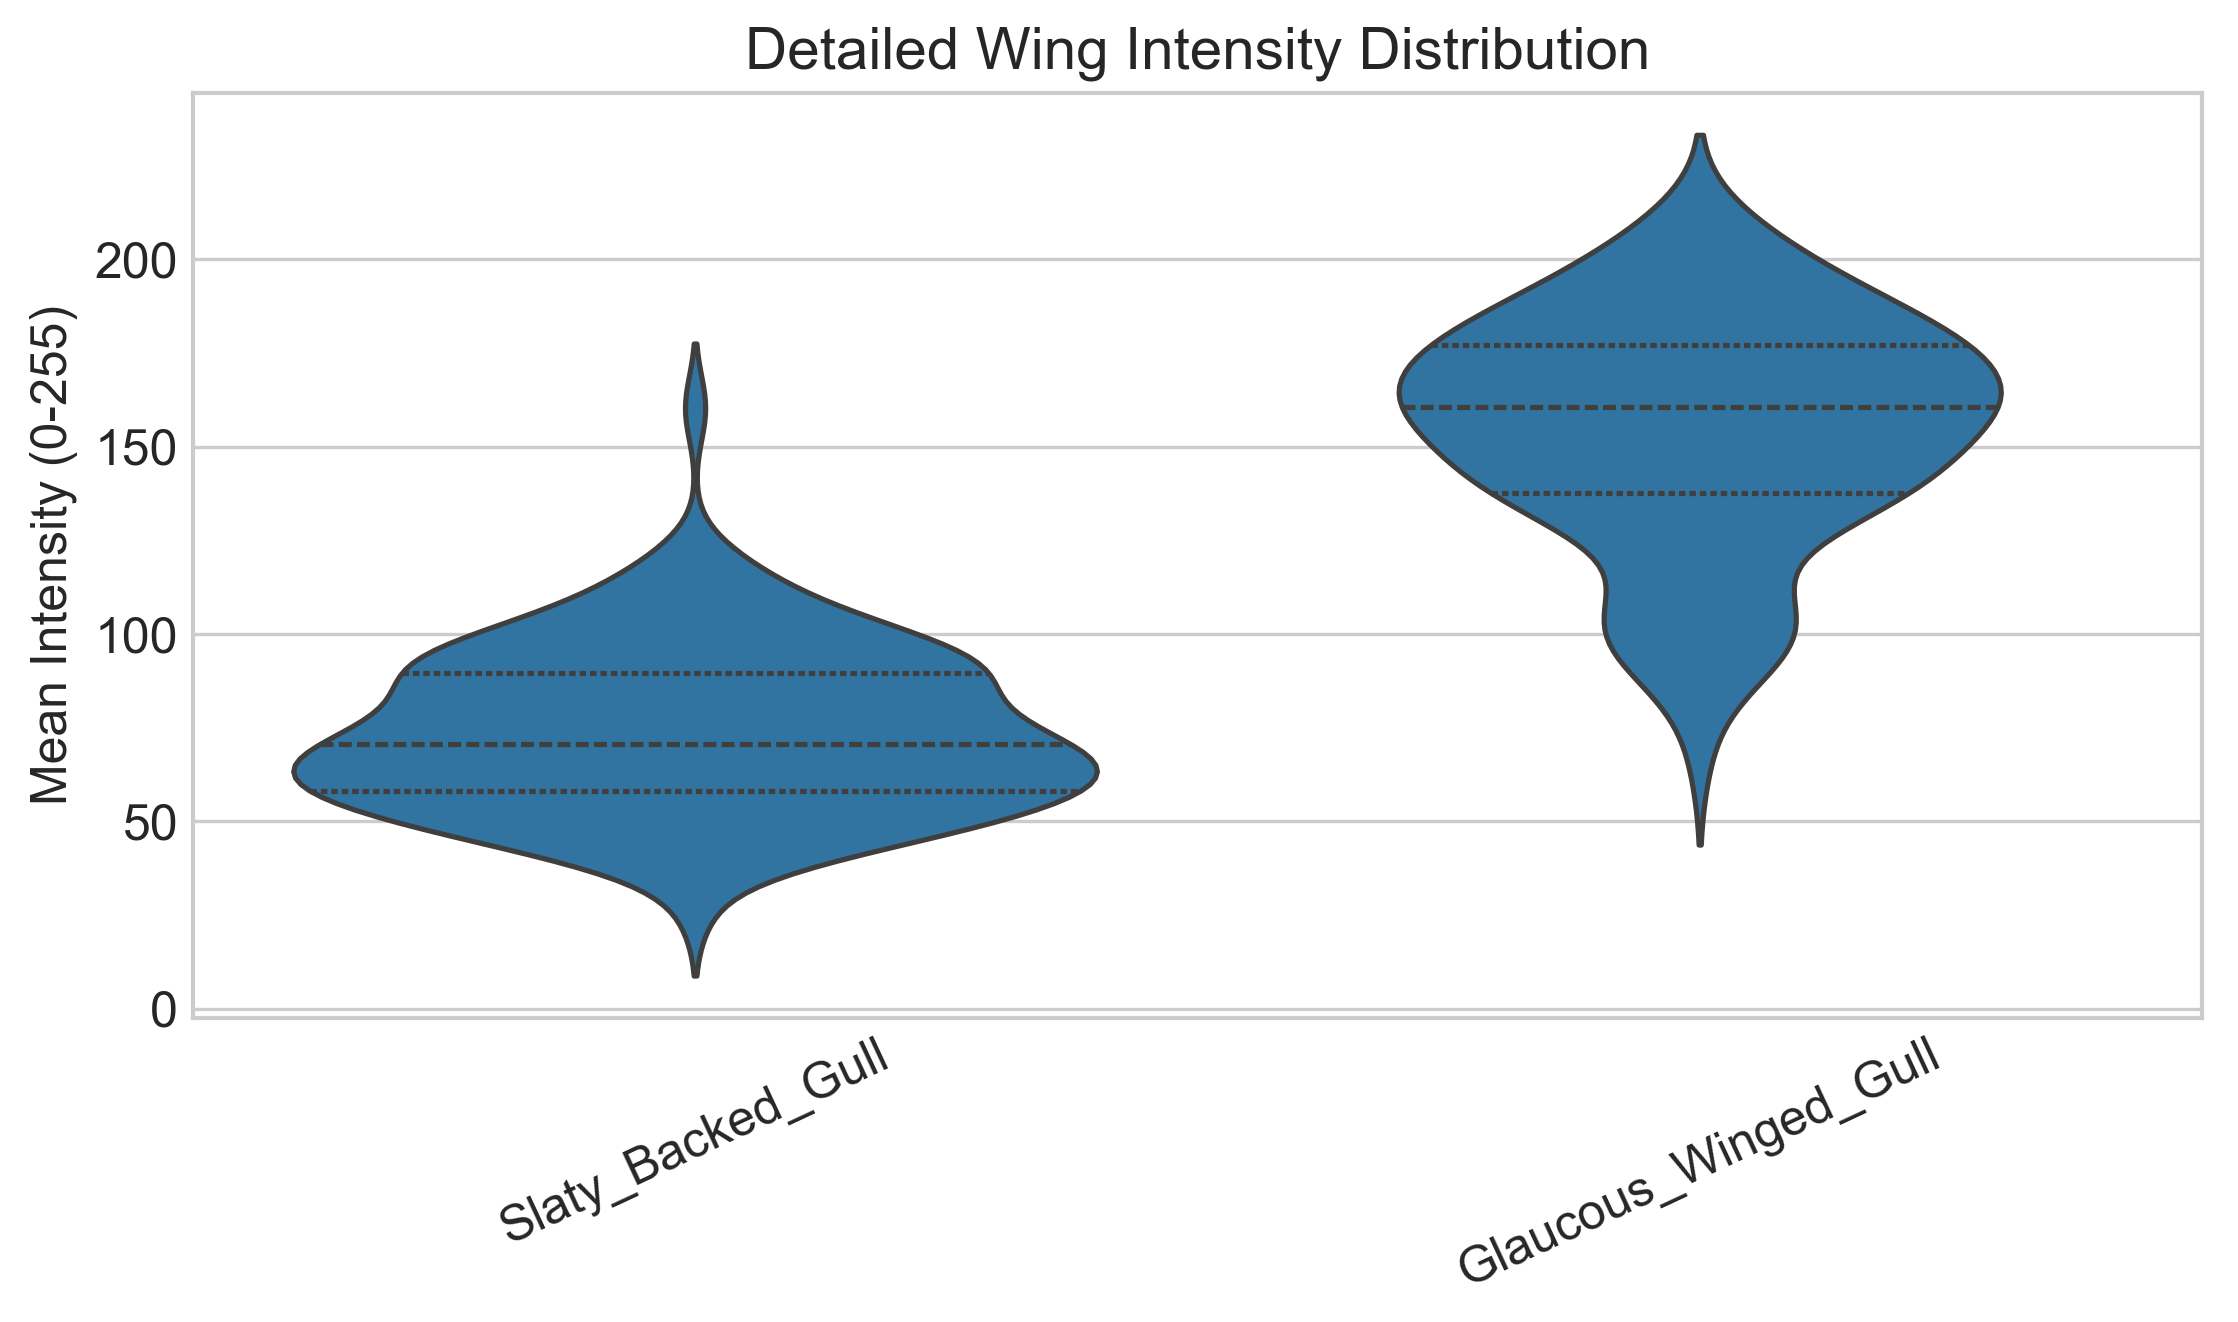
\includegraphics[width=\textwidth]{images/REPORT_IMAGES_INTENSITY/I2/wing_intensity_analysis.png}
        \caption{Comparison of wing intensity values between species.}
        \label{fig:wing_intensity}
    \end{subfigure}
    \hfill
    \begin{subfigure}[b]{0.48\textwidth}
        \centering
        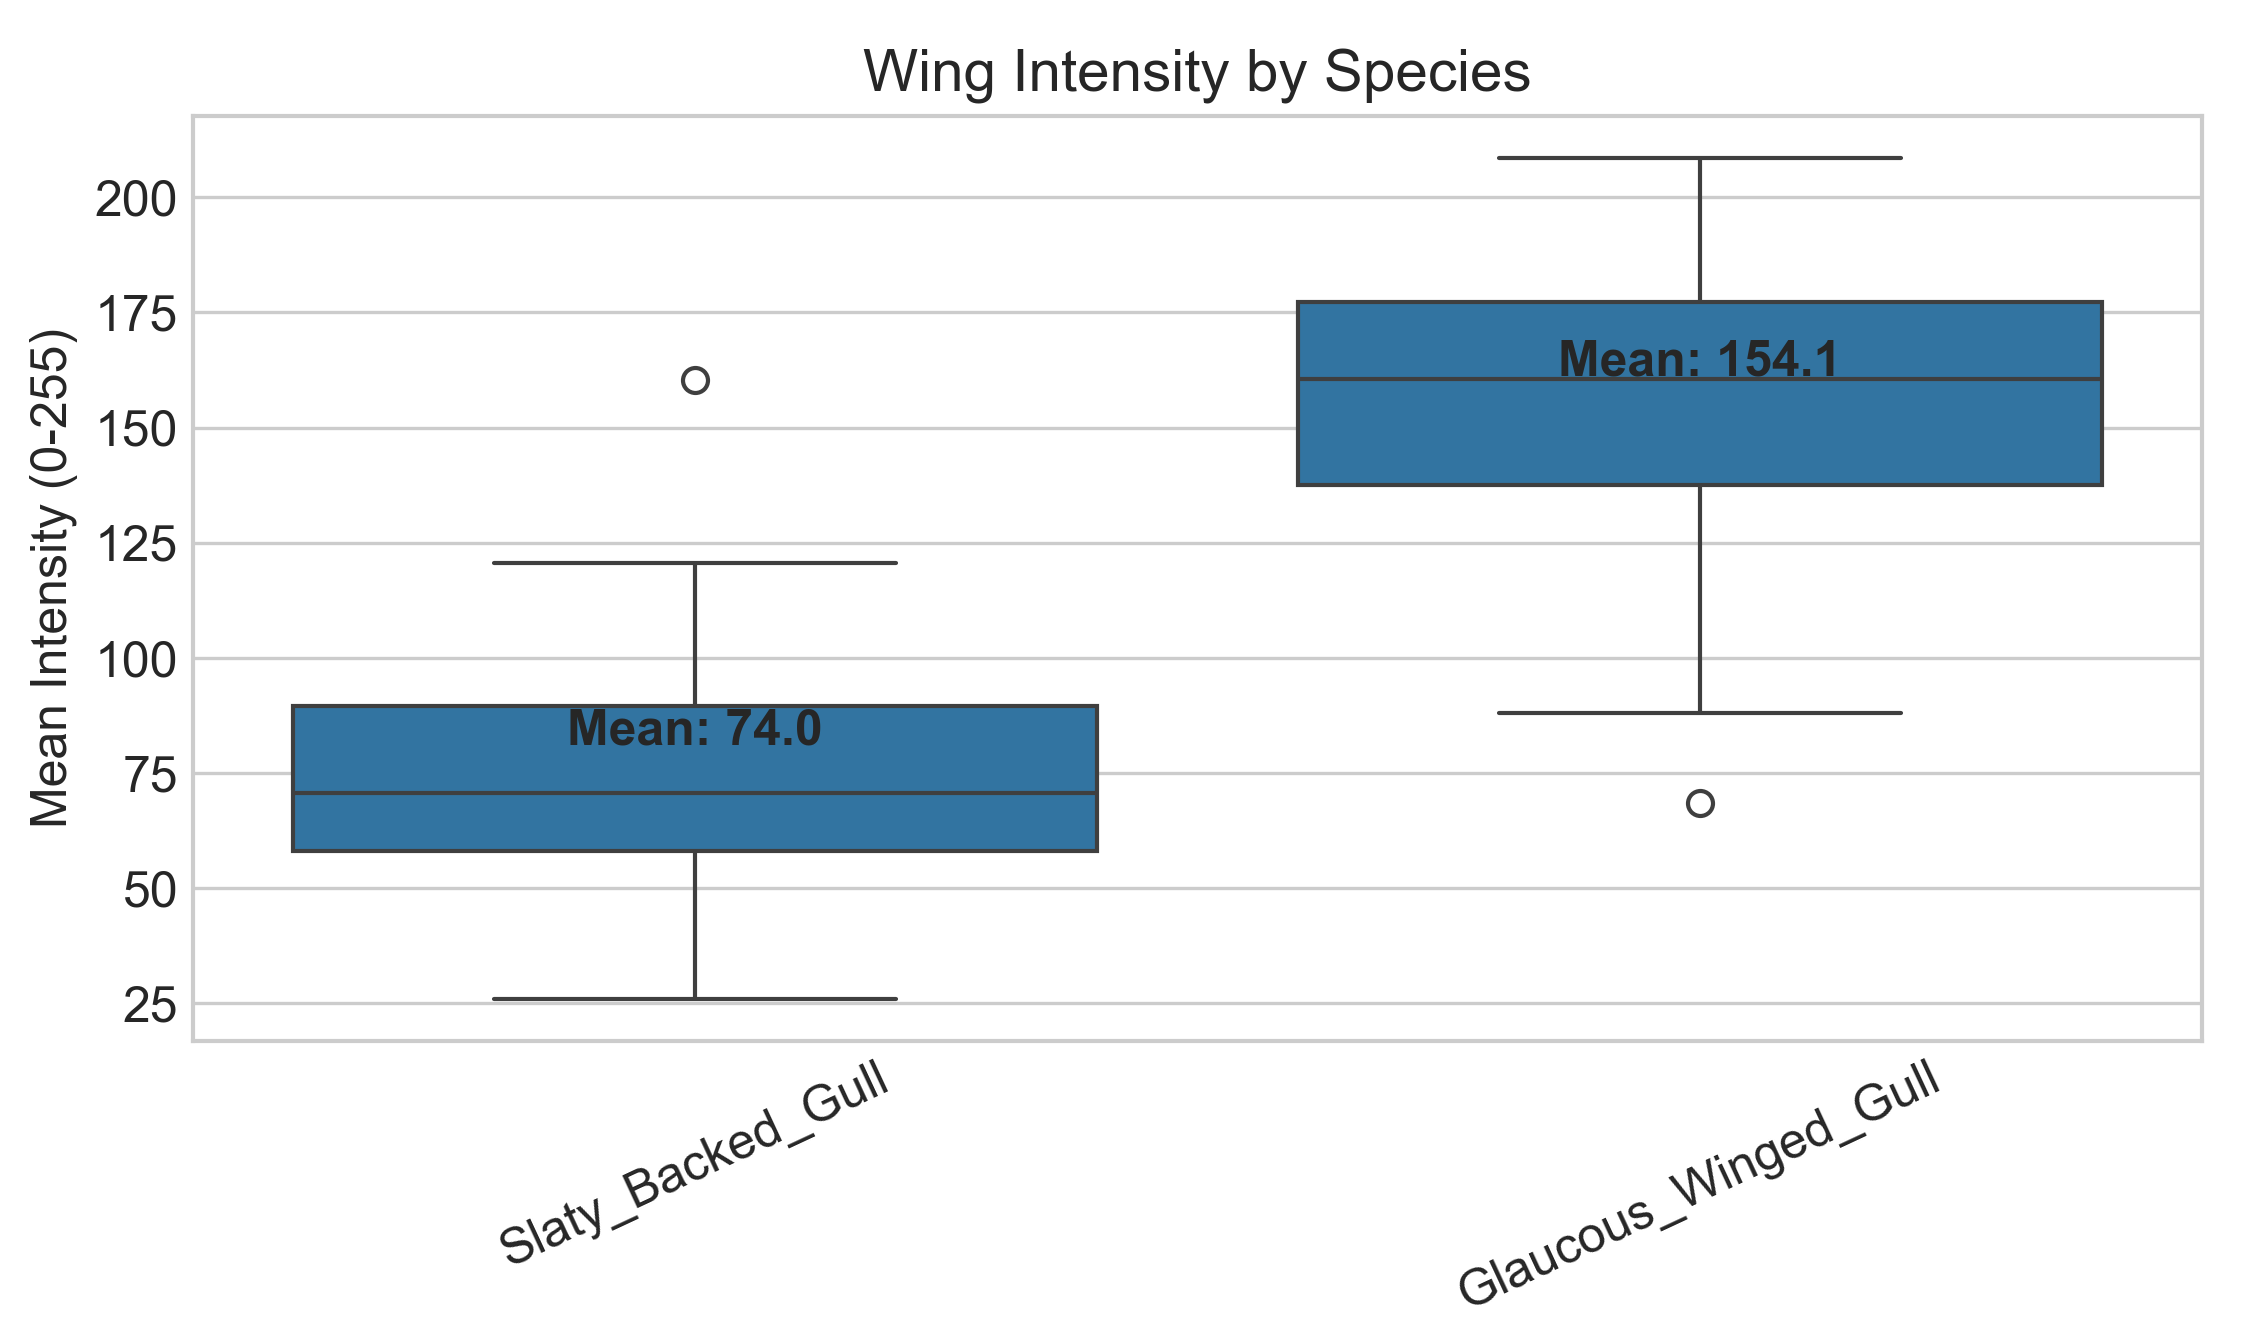
\includegraphics[width=\textwidth]{images/REPORT_IMAGES_INTENSITY/I2/WINGINTENSITY.png}
        \caption{Mean wing intensity across samples.}
        \label{fig:wing_intensity_means}
    \end{subfigure}
    \caption{Wing intensity metrics for Slaty-backed and Glaucous-winged Gulls, showing significant brightness differences.}
    \label{fig:wing_intensity_combined}
\end{figure}

\subsection{Distributions of Wing and Wingtip Intensities}

A comprehensive analysis of pixel intensity distributions in both the wing and wingtip regions reveals clear, species-specific patterns that distinguish Slaty-backed Gulls from Glaucous-winged Gulls. This section presents and interprets the observed distributions using multiple complementary metrics.

\subsection{Wing Intensity Distributions}

Figure~\ref{fig:wing_intensity_distribution} displays the distribution of mean wing intensities for both species. Slaty-backed Gulls cluster at lower mean intensity values, indicating darker wings, while Glaucous-winged Gulls are concentrated at higher mean intensities, reflecting lighter wings. The distributions are largely non-overlapping, underscoring a strong differentiation in overall wing brightness between the two species.

\begin{figure}[h]
    \centering
    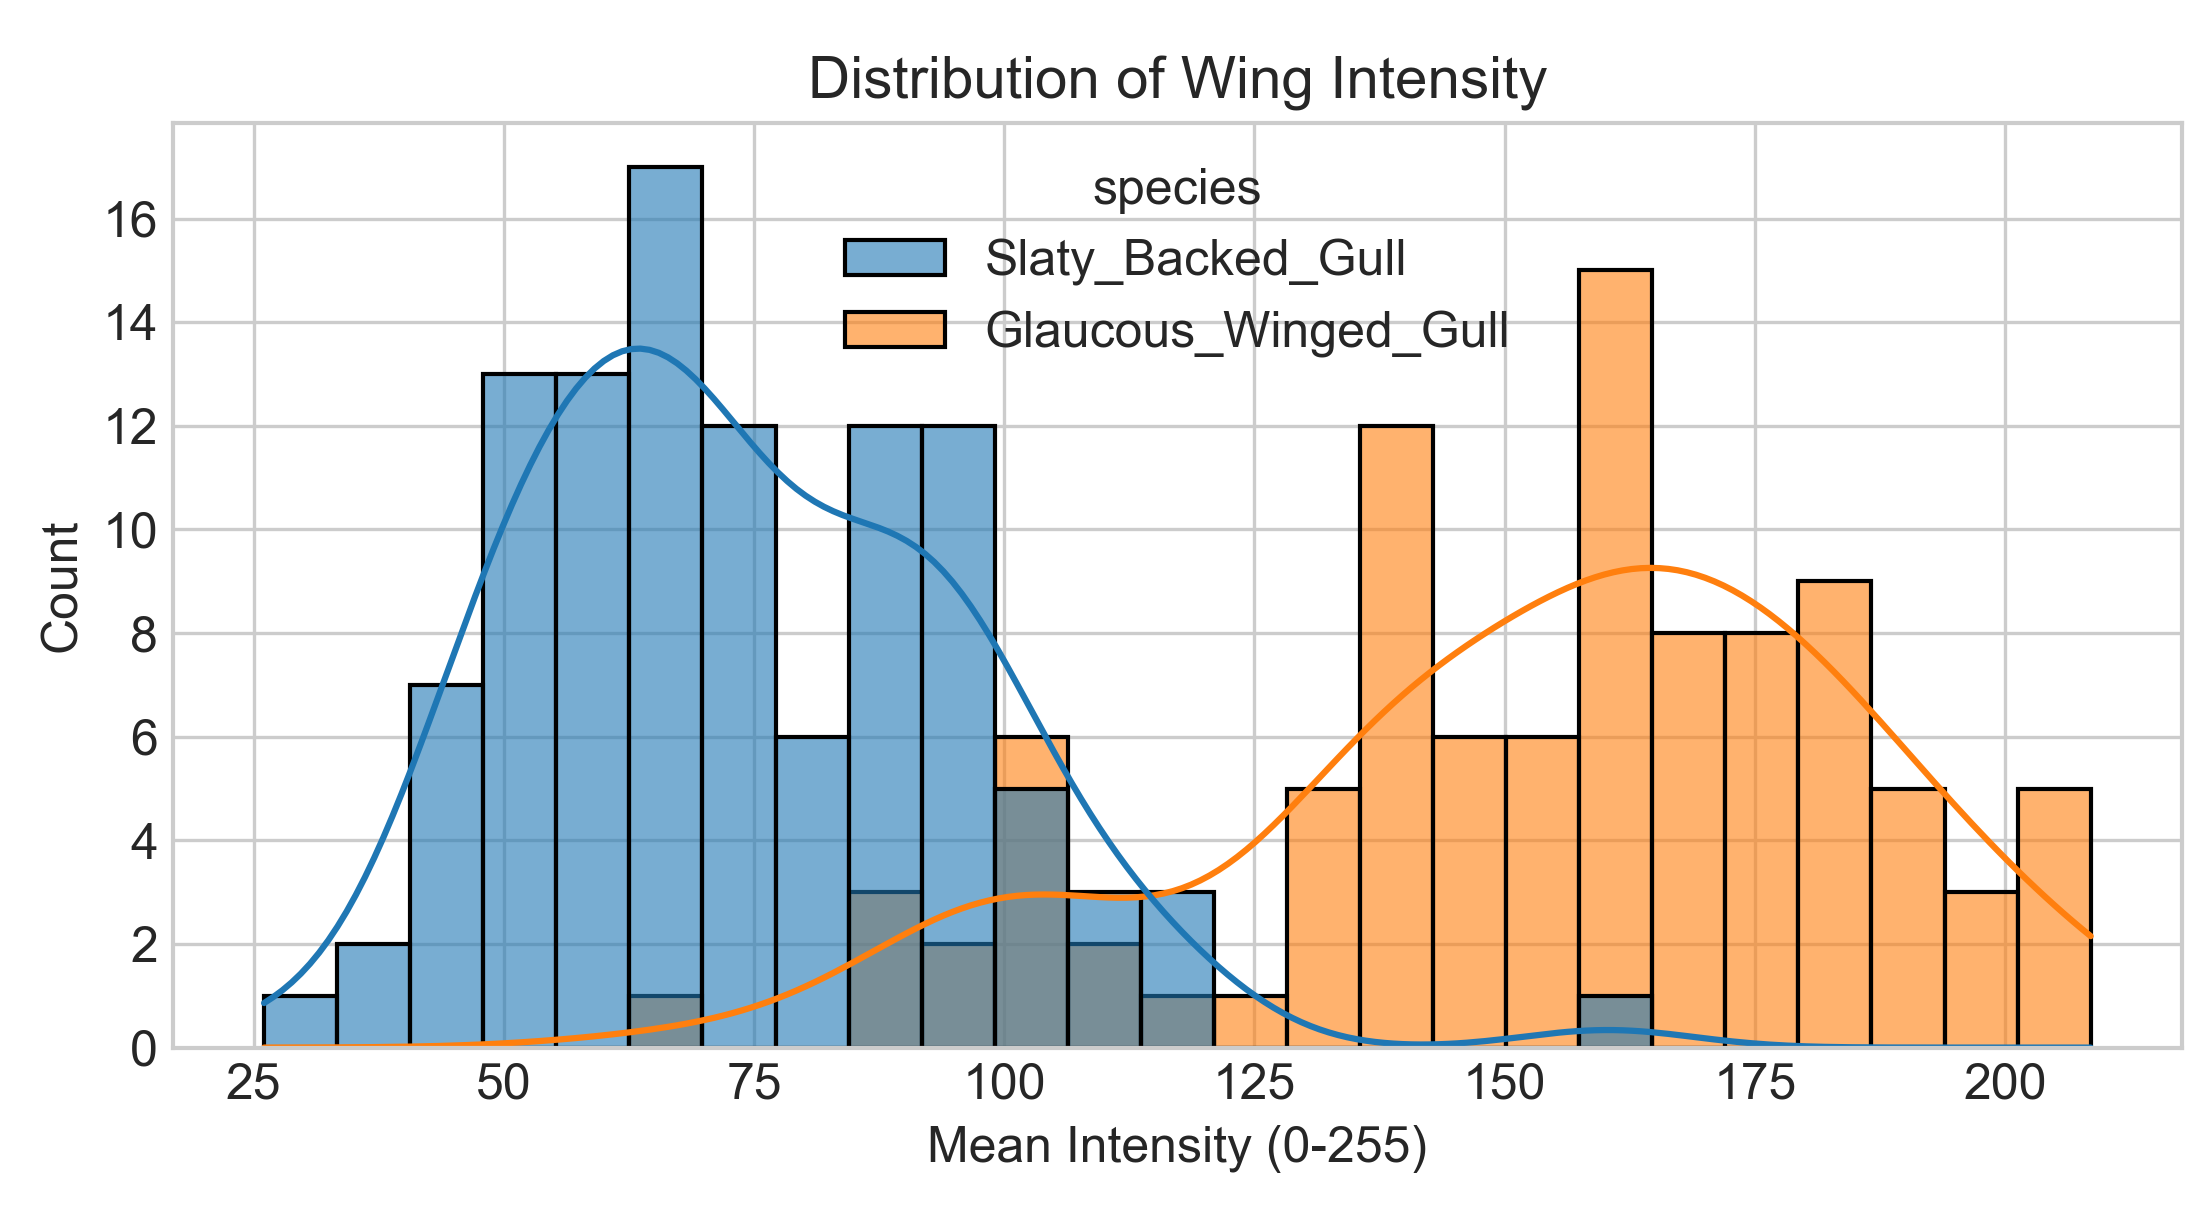
\includegraphics[width=0.55\textwidth]{images/REPORT_IMAGES_INTENSITY/I2/ditribution.png}
    \caption{Distribution of mean wing intensity for Slaty-backed Gulls (blue) and Glaucous-winged Gulls (orange). Each species forms a distinct cluster, reflecting their characteristic wing brightness.}
    \label{fig:wing_intensity_distribution}
\end{figure}


\subsection{Wingtip Pixel Intensity Distributions}

The distributions of wingtip pixel intensities for both species are shown in Figure~\ref{fig:wingtip_intensity_distributions}. Slaty-backed Gulls (orange) have a higher proportion of darker pixels (lower intensity values), while Glaucous-winged Gulls (blue) show a greater proportion of lighter pixels (higher intensity values). Both grouped and fine-grained binning approaches reveal unique, largely non-overlapping patterns for each species.

\begin{figure}[h]
    \centering
    \begin{subfigure}[b]{0.47\textwidth}
        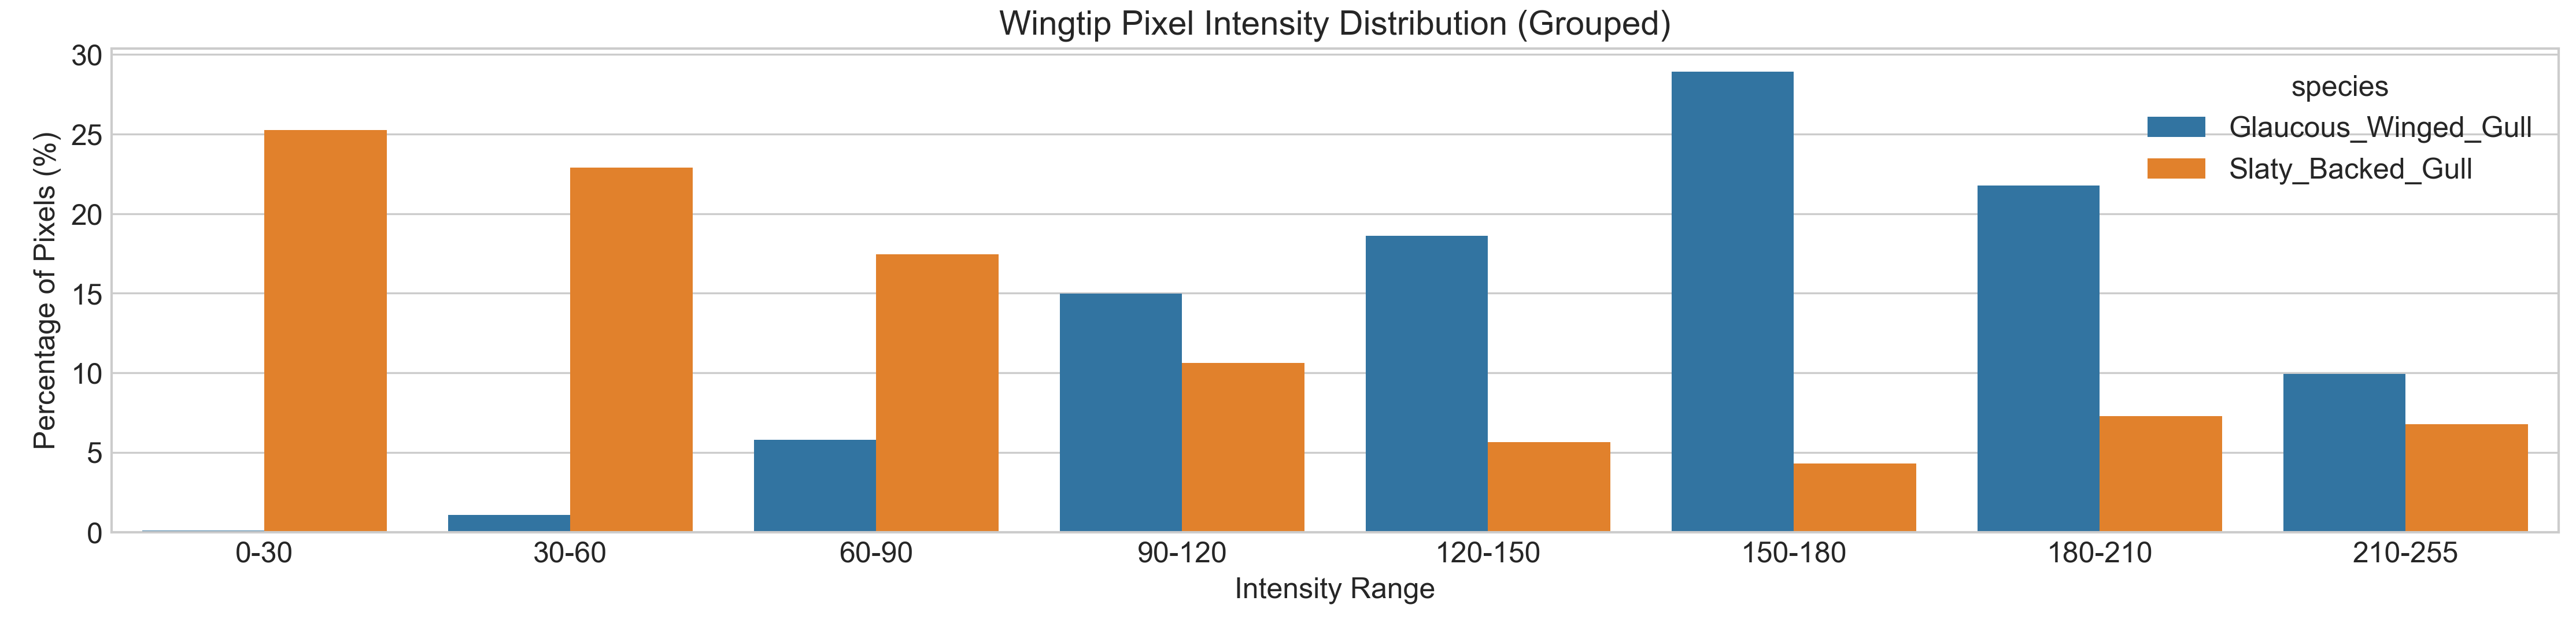
\includegraphics[width=\textwidth]{images/REPORT_IMAGES_INTENSITY/I2/intensitydistribution.png}
        \caption{Grouped intensity bins}
        \label{fig:wingtip_intensity_distribution_grouped}
    \end{subfigure}
    \hfill
    \begin{subfigure}[b]{0.47\textwidth}
        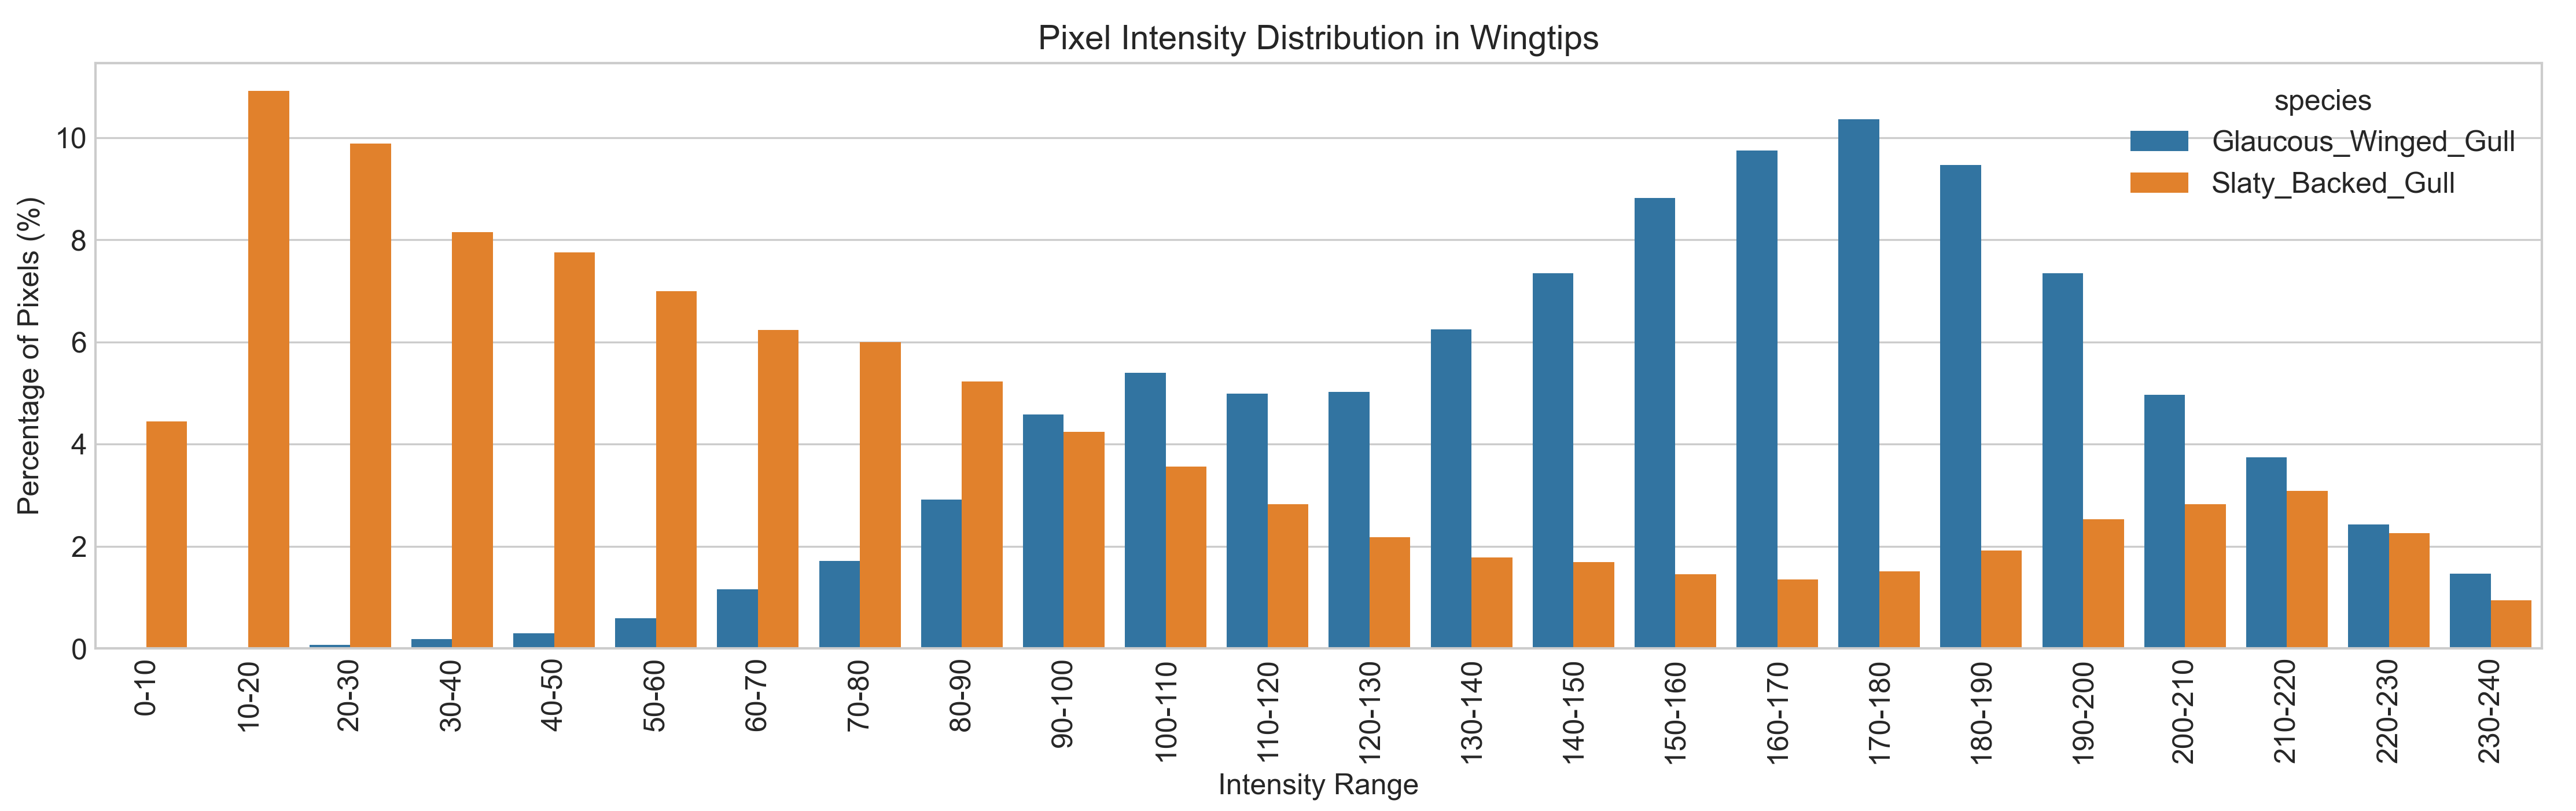
\includegraphics[width=\textwidth]{images/REPORT_IMAGES_INTENSITY/I2/TIPdistribution.png}
        \caption{Fine-grained intensity bins}
        \label{fig:wingtip_intensity_distribution_fine}
    \end{subfigure}
    \caption{Distributions of wingtip pixel intensities for Slaty-backed Gulls (orange) and Glaucous-winged Gulls (blue) using (a) grouped and (b) fine-grained intensity bins.}
    \label{fig:wingtip_intensity_distributions}
\end{figure}

\subsection{Presence of Very Dark Pixels}

A detailed analysis of wingtip pixel intensity reveals a striking difference in the prevalence of very dark pixels between Slaty-backed Gulls and Glaucous-winged Gulls. As shown in Figure~\ref{fig:pixels_below_thresh}, Slaty-backed Gulls have a much higher percentage of wingtip pixels below each intensity threshold examined ($<$30, $<$40, $<$50, $<$60), with values rising from 25\% to nearly 48\%. In contrast, Glaucous-winged Gulls have negligible proportions of such dark pixels at all thresholds.

Figure~\ref{fig:verydarkdist} further demonstrates that this difference is consistent across all sub-ranges within the very dark pixel spectrum (0--60), with Slaty-backed Gulls consistently showing a substantially greater percentage of pixels in each bin.


\begin{figure}[H]
    \centering
    \begin{subfigure}[b]{0.48\textwidth}
        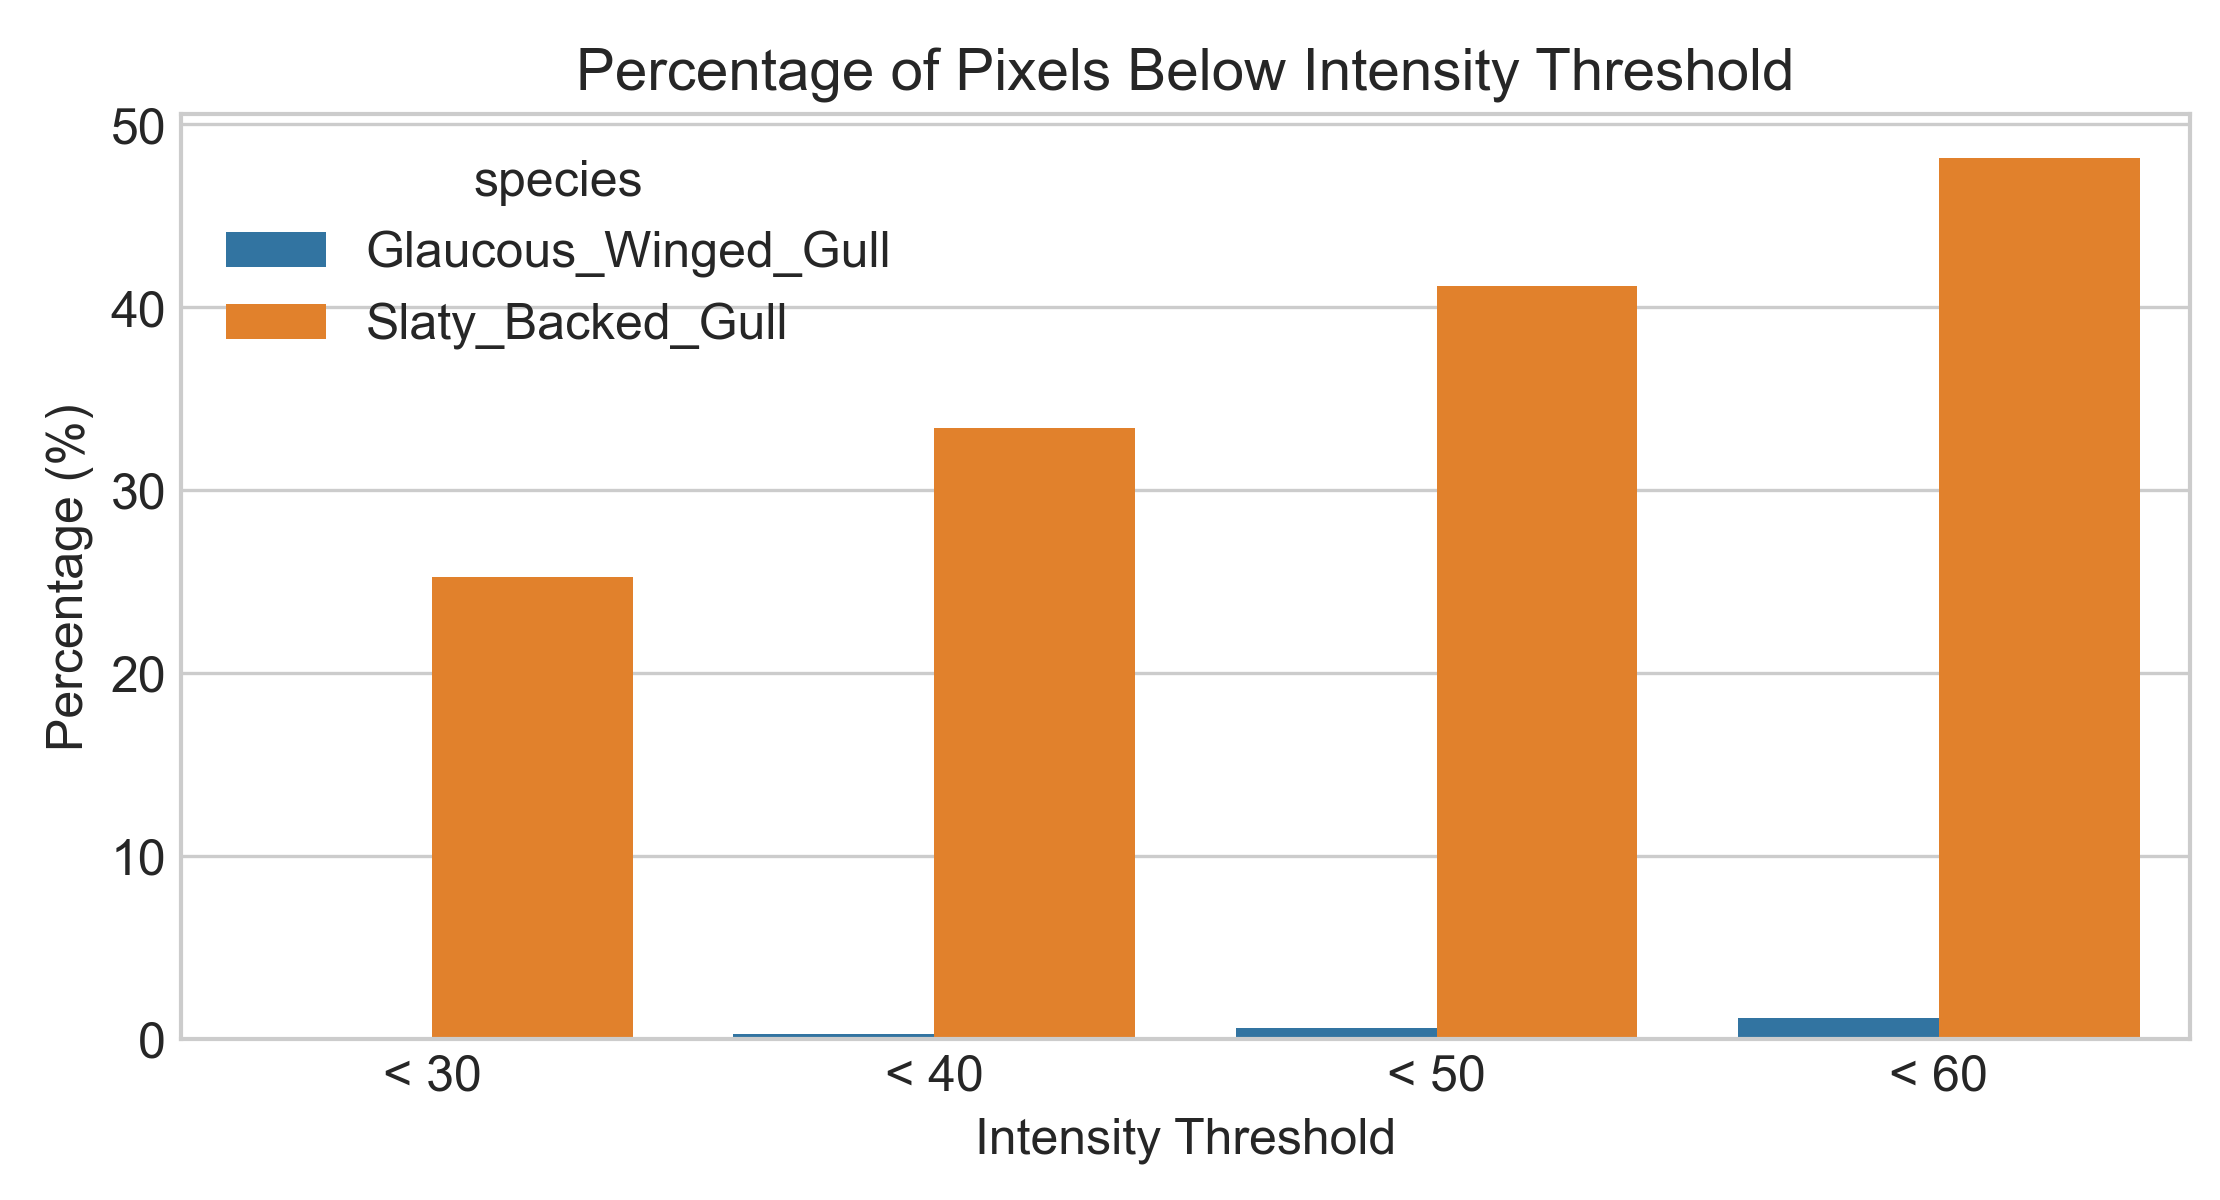
\includegraphics[width=\textwidth]{images/REPORT_IMAGES_INTENSITY/I2/pixelsbelowthresh.png}
        \caption{Percentage of wingtip pixels below each intensity threshold.}
        \label{fig:pixels_below_thresh}
    \end{subfigure}
    \hfill
    \begin{subfigure}[b]{0.48\textwidth}
        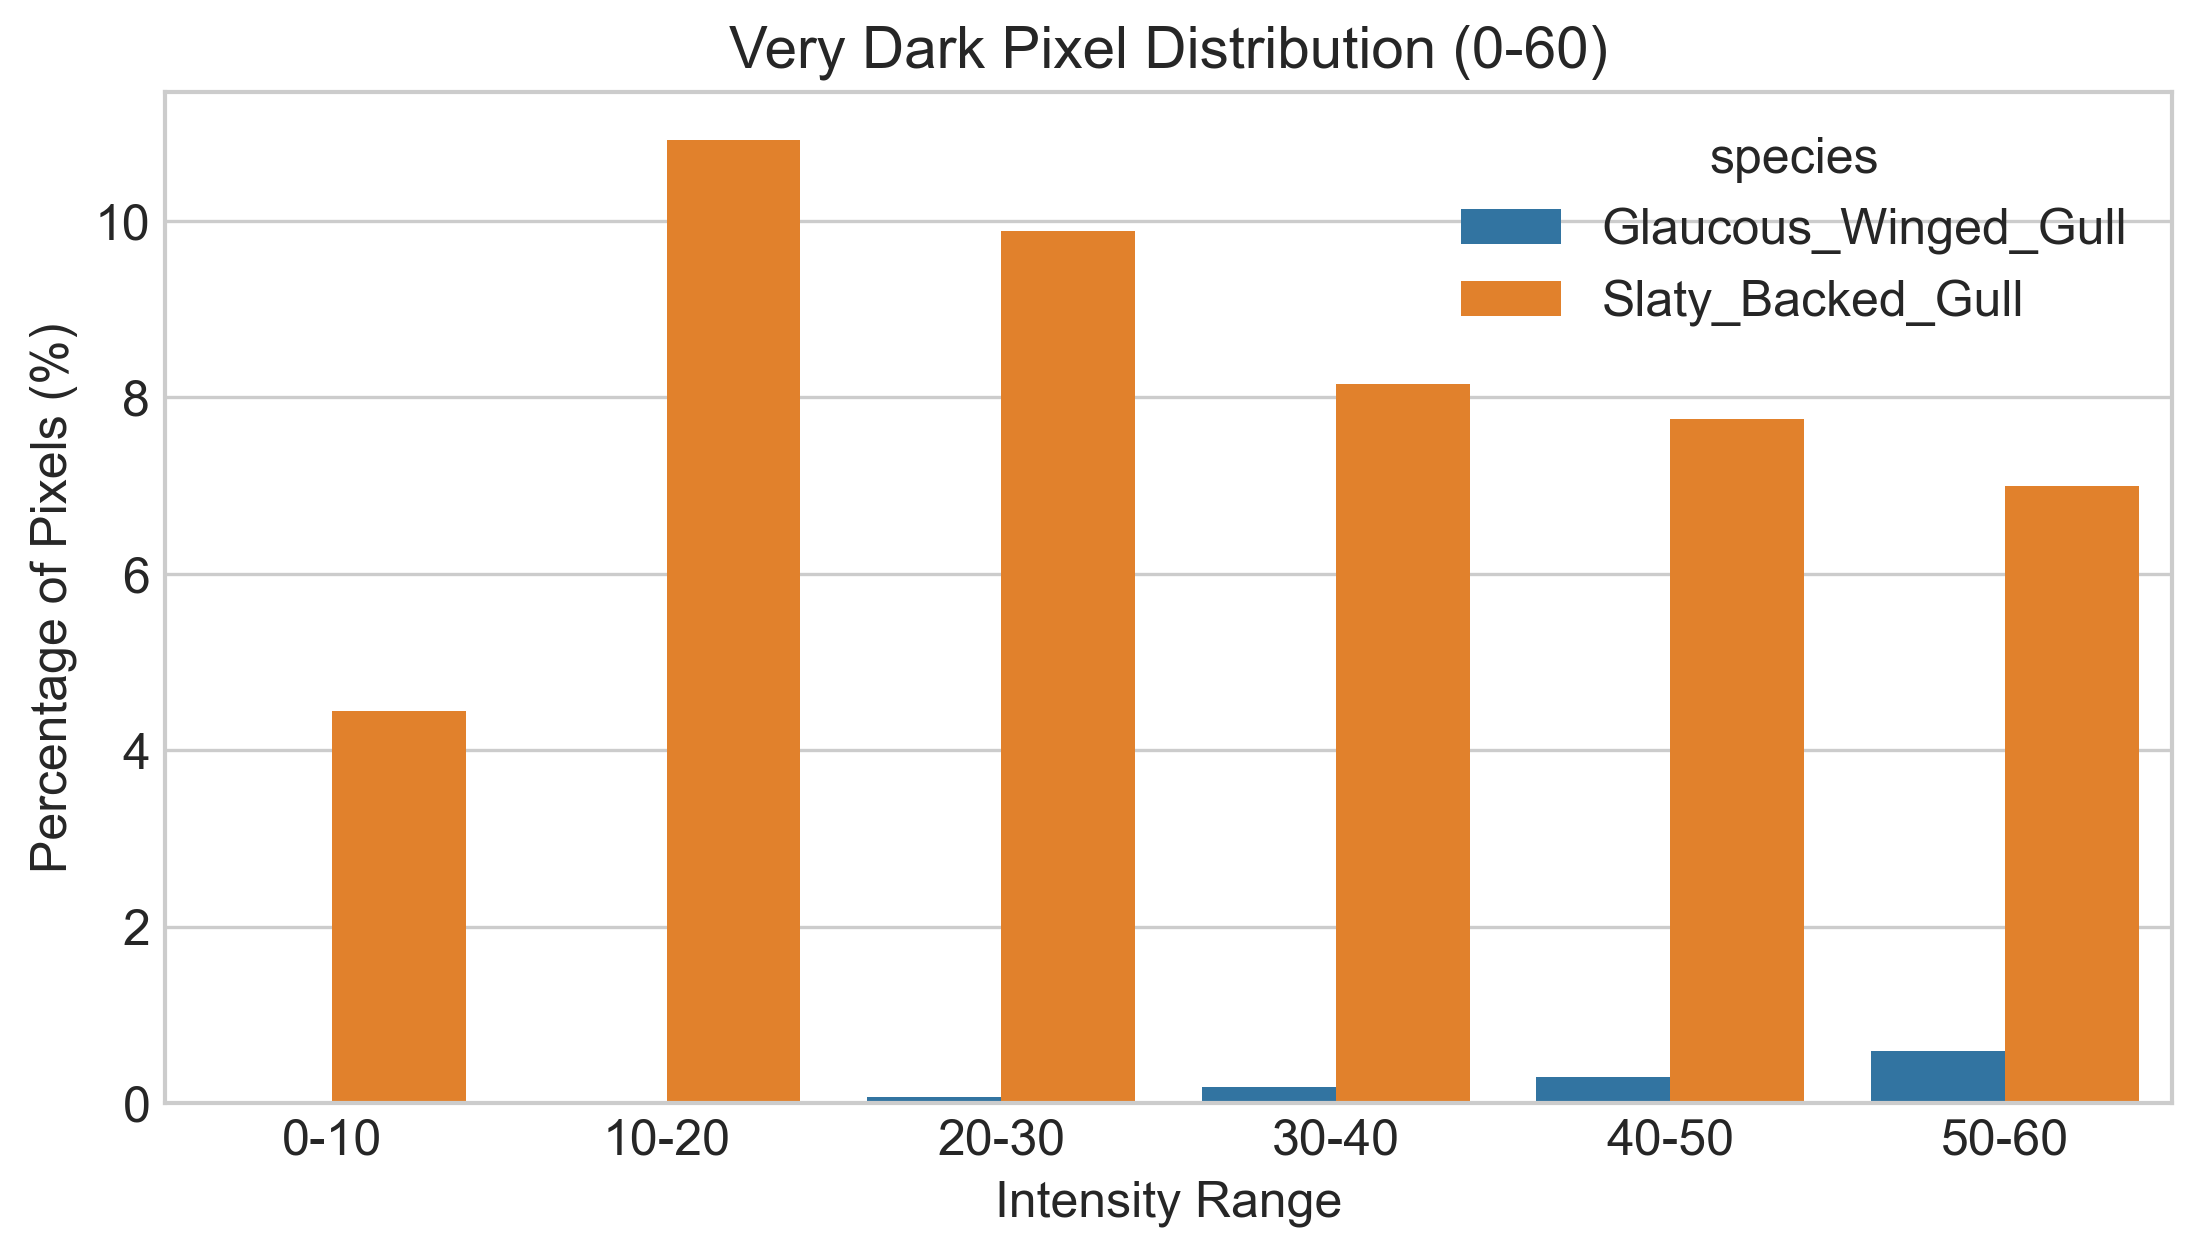
\includegraphics[width=\textwidth]{images/REPORT_IMAGES_INTENSITY/I2/verydarkdist.png}
        \caption{Distribution of very dark pixels (0--60) in wingtip regions.}
        \label{fig:verydarkdist}
    \end{subfigure}
    \caption{Comparison of very dark pixel proportions in wingtip regions for Slaty-backed and Glaucous-winged Gulls.}
\end{figure}

\begin{figure}[H]
    \centering
    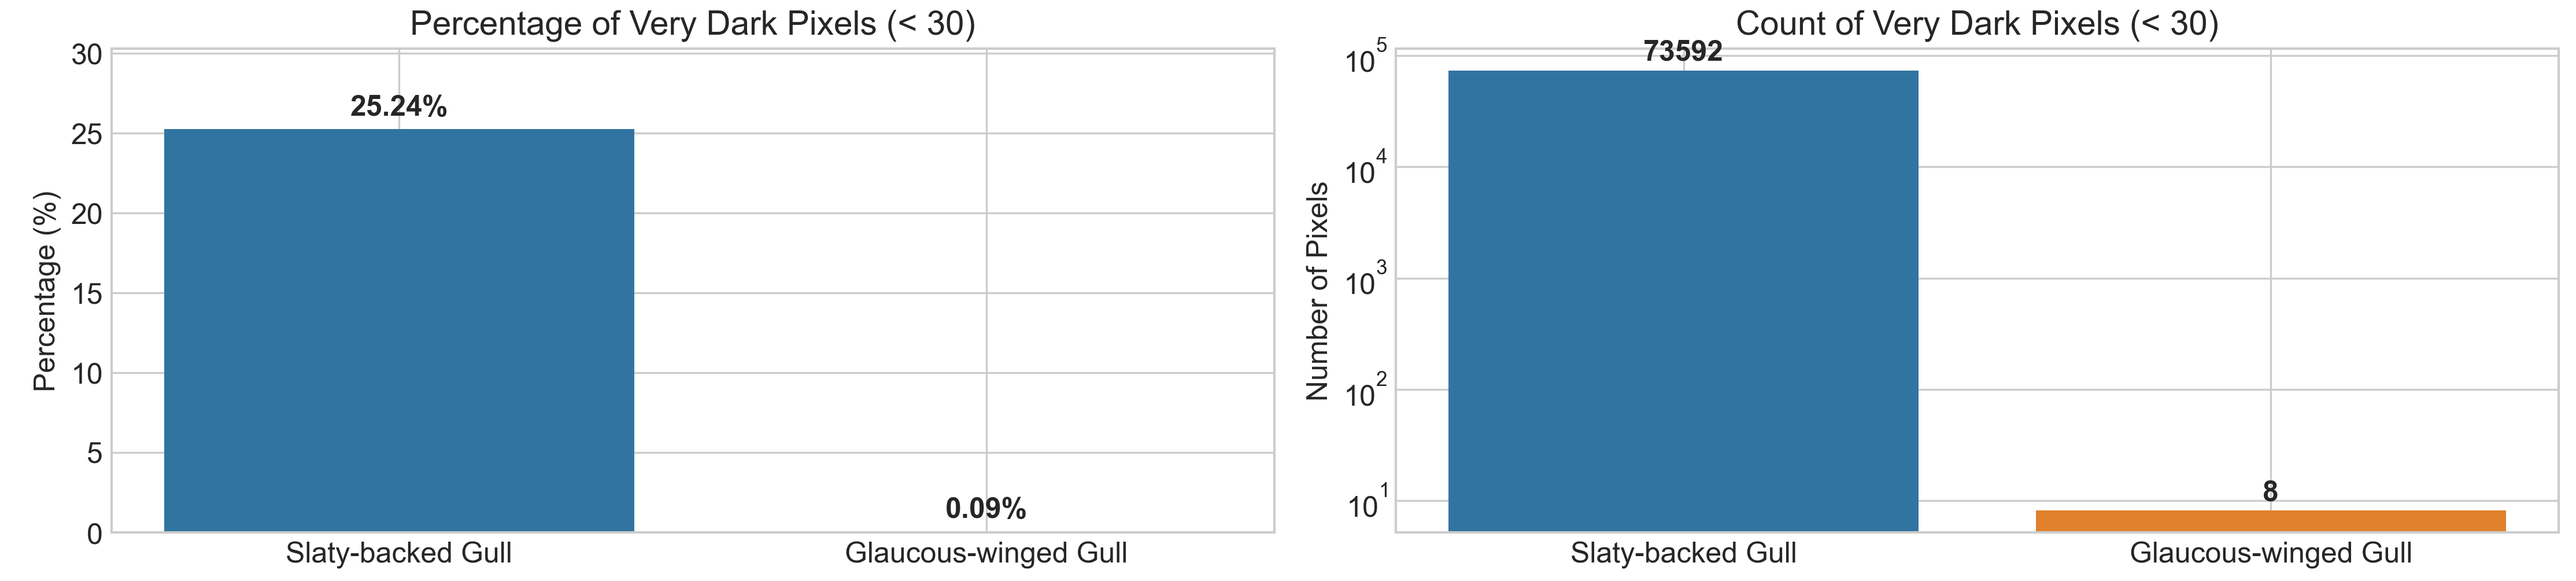
\includegraphics[width=0.9\textwidth]{images/REPORT_IMAGES_INTENSITY/I2/darkpixels.png}
    \caption{Left: Percentage of very dark pixels ($<$30) by species. Right: Average count of very dark pixels ($<$30) per wingtip region, shown on a logarithmic scale.}
    \label{fig:darkpixels}
\end{figure}

These results demonstrate that the presence and abundance of very dark pixels in the wingtip region are highly distinctive for Slaty-backed Gulls, providing a robust quantitative feature for differentiating them from Glaucous-winged Gulls.

\subsection{Relationship Between Wing and Wingtip Intensities}

To quantitatively assess the relative darkness of wingtip area compared to the rest of the wing which were the 2 critical areas highlighted by Grad-CAM, the proportion of wingtip pixels that are darker than the mean wing intensity for each species was calculated as suggested by industry expert.


\begin{table}[H]
    \centering
    \caption{Proportion of Wingtip Pixels Darker than Mean Wing Intensity}
    \label{tab:darknessproportion}
    \begin{tabular}{lcc}
        \toprule
        Species & Percentage \\
        \midrule
        Slaty-backed Gull & 56.69\% \\
        Glaucous-winged Gull & 47.71\% \\
        \bottomrule
    \end{tabular}
\end{table}

Figure~\ref{fig:wing_vs_wingtip_intensity} visualizes the relationship between mean wing intensity and mean wingtip intensity for individual birds. The dashed line indicates equal intensity between wing and wingtip. As illustrated, there is a strong positive correlation between wing and wingtip intensities across both species; as the mean wing intensity increases, the mean wingtip intensity also increases. This pattern suggests that, in most cases, the relative difference in darkness between the wing and wingtip results only in a slight difference in the proportion of darker wingtip pixels between the two species.

\begin{figure}[h]
    \centering
    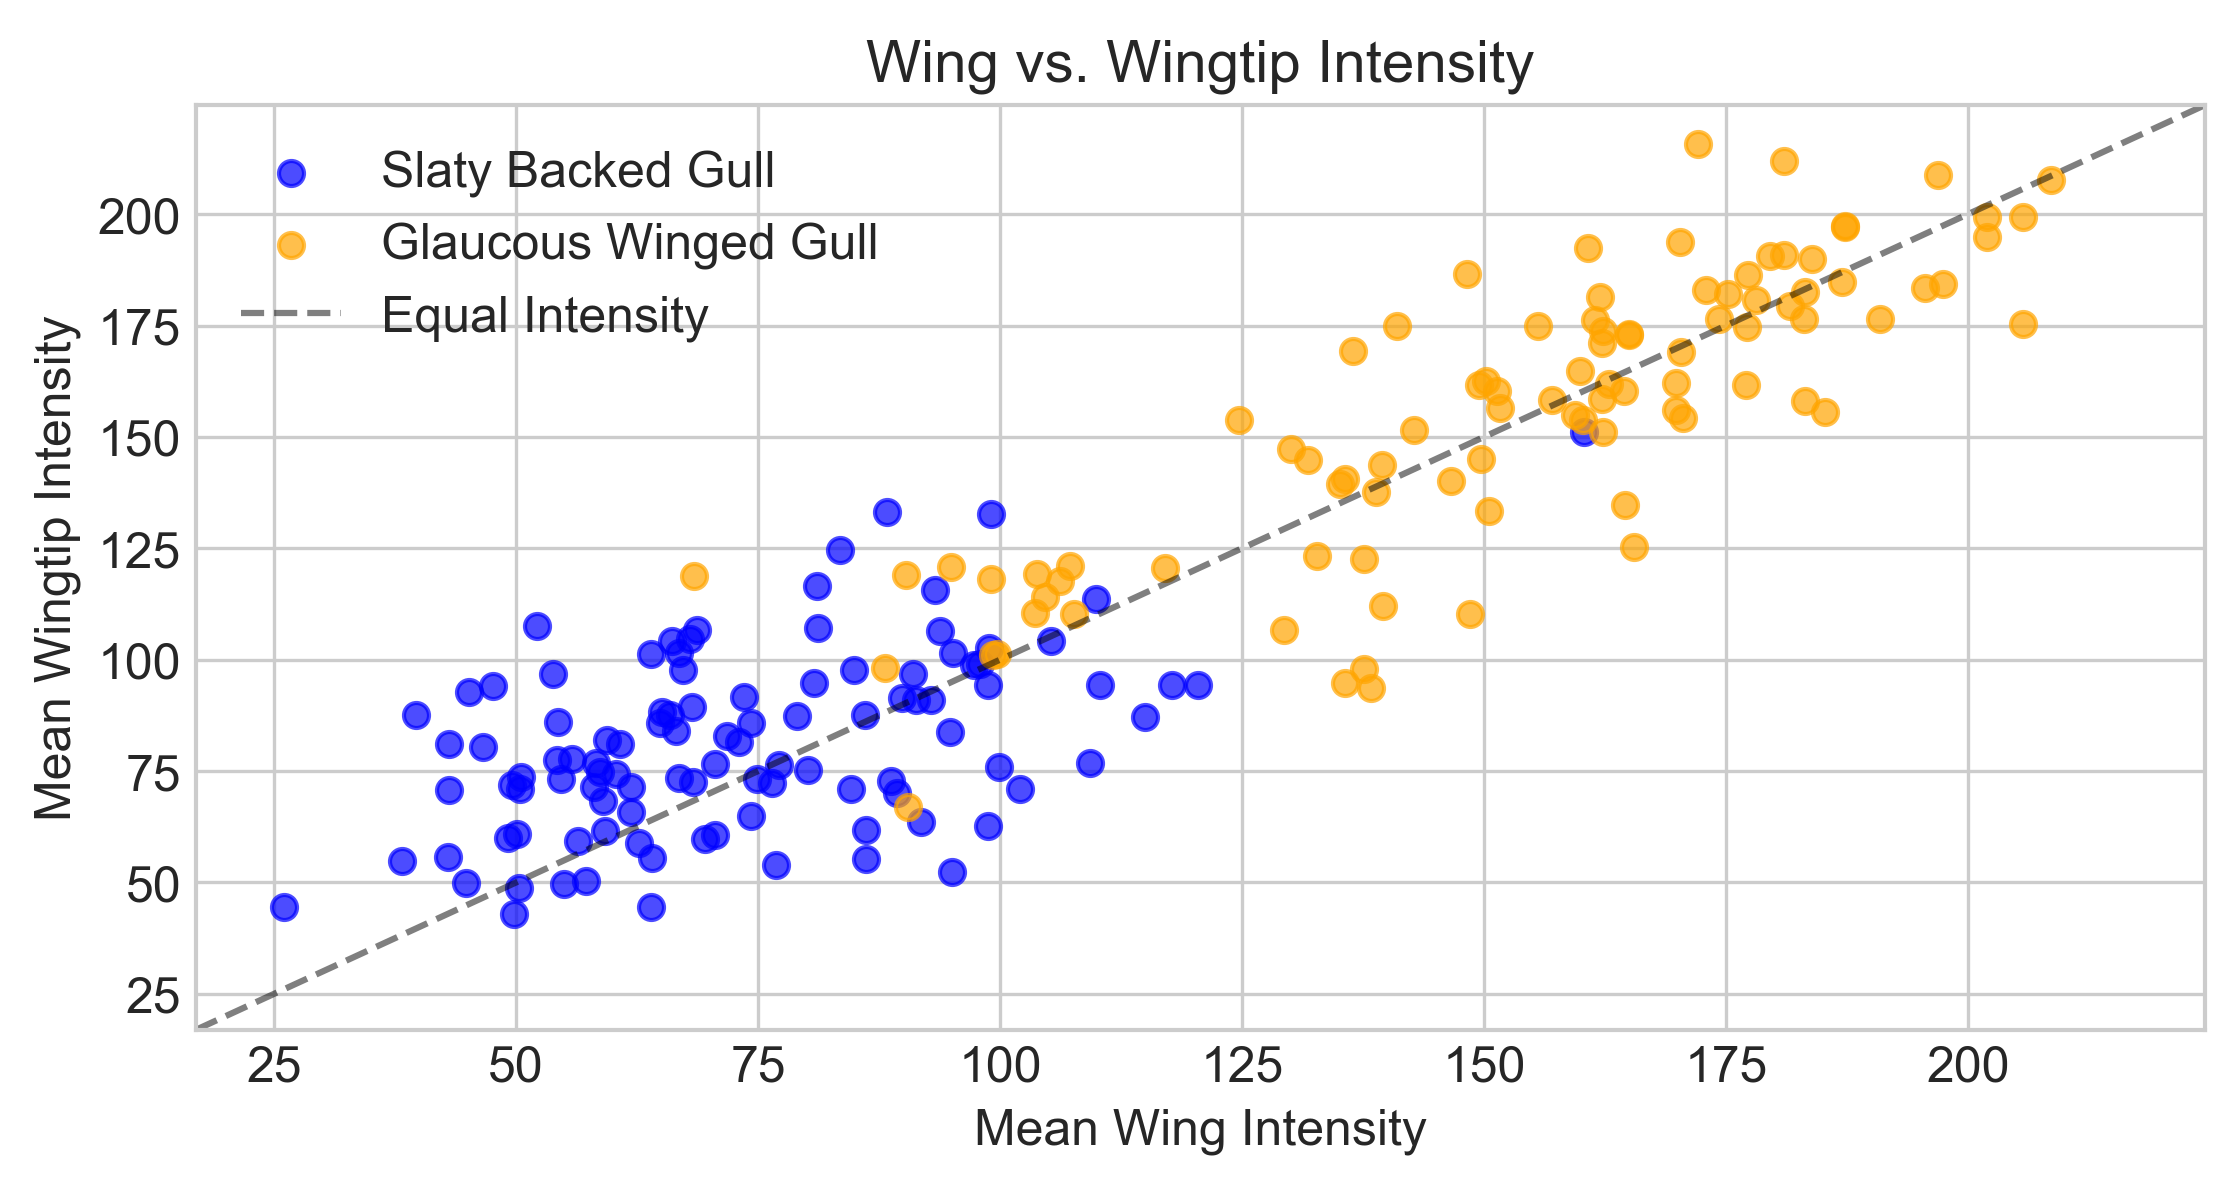
\includegraphics[width=0.55\textwidth]{images/REPORT_IMAGES_INTENSITY/I2/clusterwingwingtip.png}
    \caption{Scatter plot of mean wing intensity vs. mean wingtip intensity for Slaty-backed Gulls (blue) and Glaucous-winged Gulls (orange). The dashed line indicates equal intensity between wing and wingtip.}
    \label{fig:wing_vs_wingtip_intensity}
\end{figure}


\subsection{Wingtip Contrast and Darkness Feature Comparison}

To comprehensively compare the wingtip characteristics distinguishing Slaty-backed and Glaucous-winged Gulls, we analyzed two key features: (1) the proportion of wingtip pixels that are darker than the wing by varying intensity thresholds, and (2) the proportion of pixels that are absolutely dark, below fixed intensity values.

Figure~\ref{fig:wingtip_darkness_summary} presents a set of visualizations summarizing these metrics for both species. The heatmap in subfigure~\ref{fig:intensity_heatmap} displays, on the left, the percentage of wingtip pixels darker than the wing by various thresholds, and on the right, the percentage of absolutely dark pixels. Subfigure~\ref{fig:diff_bar} shows the absolute difference in the proportion of dark pixels between species at each threshold, while subfigure~\ref{fig:diff_curve} plots the difference curve (Slaty-backed minus Glaucous-winged) across thresholds, highlighting where the species gap is largest. Subfigure~\ref{fig:ratio_plot} quantifies the relative difference by showing the ratio of dark pixel proportions (Slaty-backed/Glaucous-winged) at each threshold, with the ratio peaking near 2.8--2.9$\times$ between thresholds of 50 and 80. Collectively, these visualizations demonstrate that Slaty-backed Gulls consistently have a much higher proportion of both strongly contrasting and absolutely dark pixels, making these features highly discriminative.

\begin{figure}[H]
    \centering
    % (a) Heatmap
    \begin{subfigure}[b]{0.48\textwidth}
        \centering
        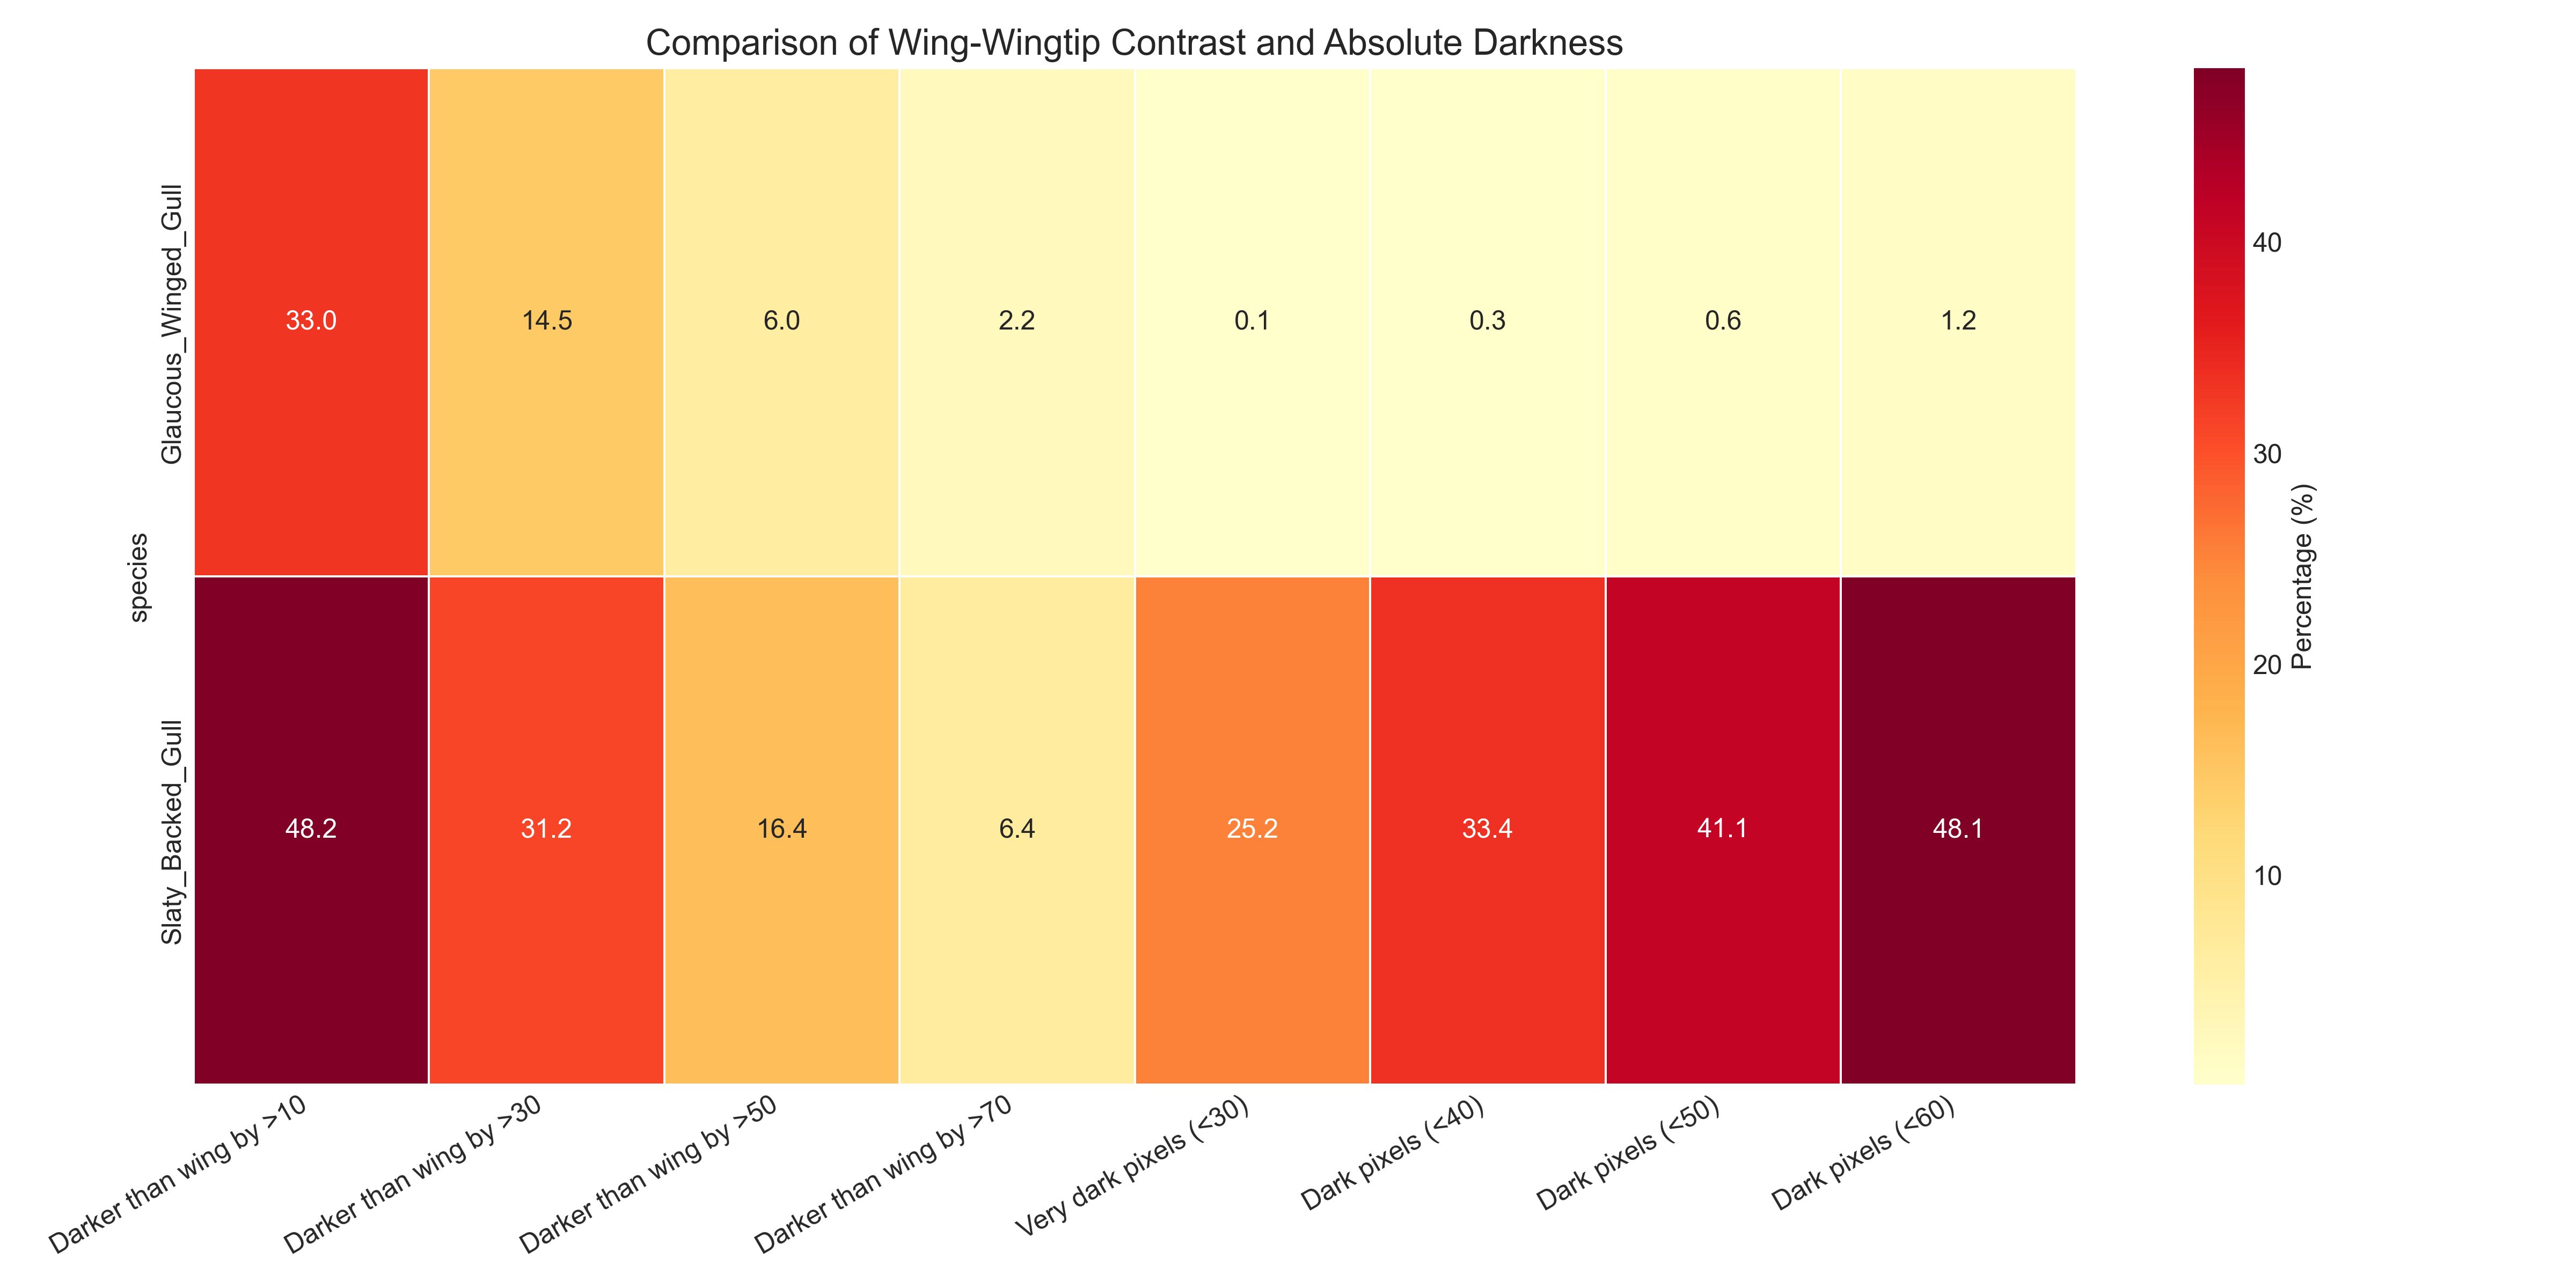
\includegraphics[width=\textwidth]{images/REPORT_IMAGES_INTENSITY/I1/wingtip_darkness_heatmap.png}
        \caption{Heatmap of wingtip darkness and contrast features for each species.}
        \label{fig:intensity_heatmap}
    \end{subfigure}
    \hfill
    % (b) Difference bar plot
    \begin{subfigure}[b]{0.48\textwidth}
        \centering
        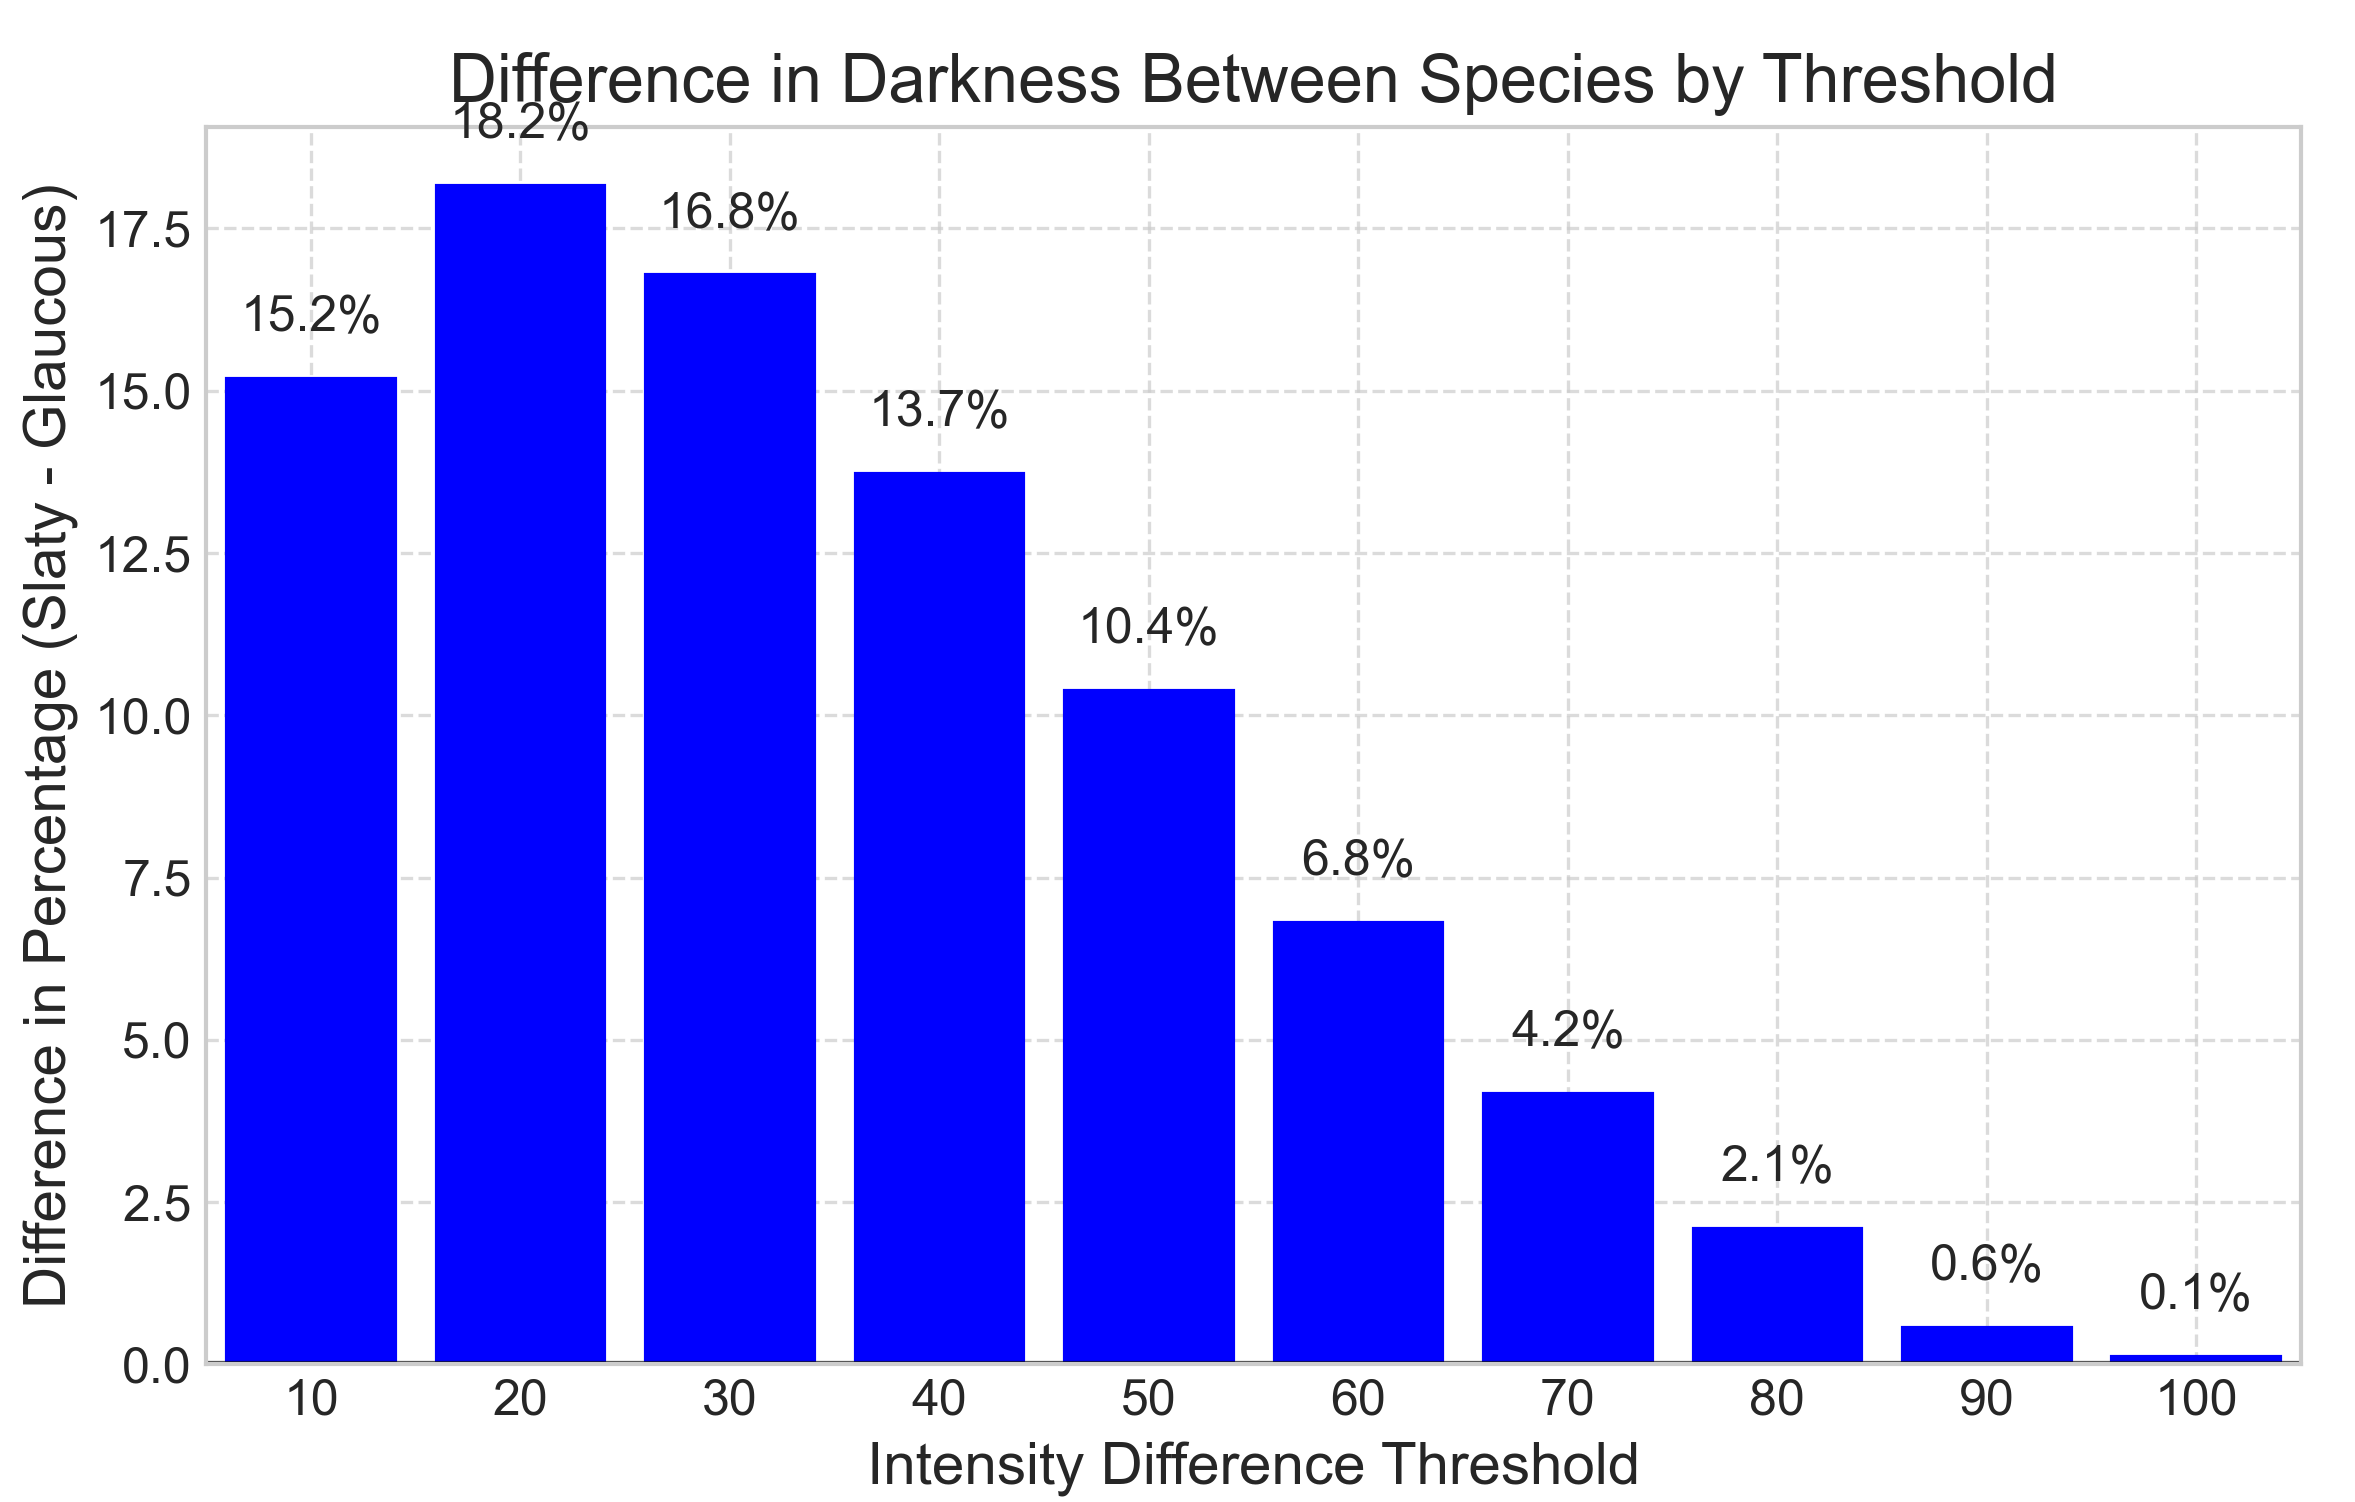
\includegraphics[width=\textwidth]{images/REPORT_IMAGES_INTENSITY/I1/diffbythresh.png}
        \caption{Absolute difference in percentage of dark pixels by threshold.}
        \label{fig:diff_bar}
    \end{subfigure}
    \vspace{1em}
    % (c) Difference curve
    \begin{subfigure}[b]{0.48\textwidth}
        \centering
        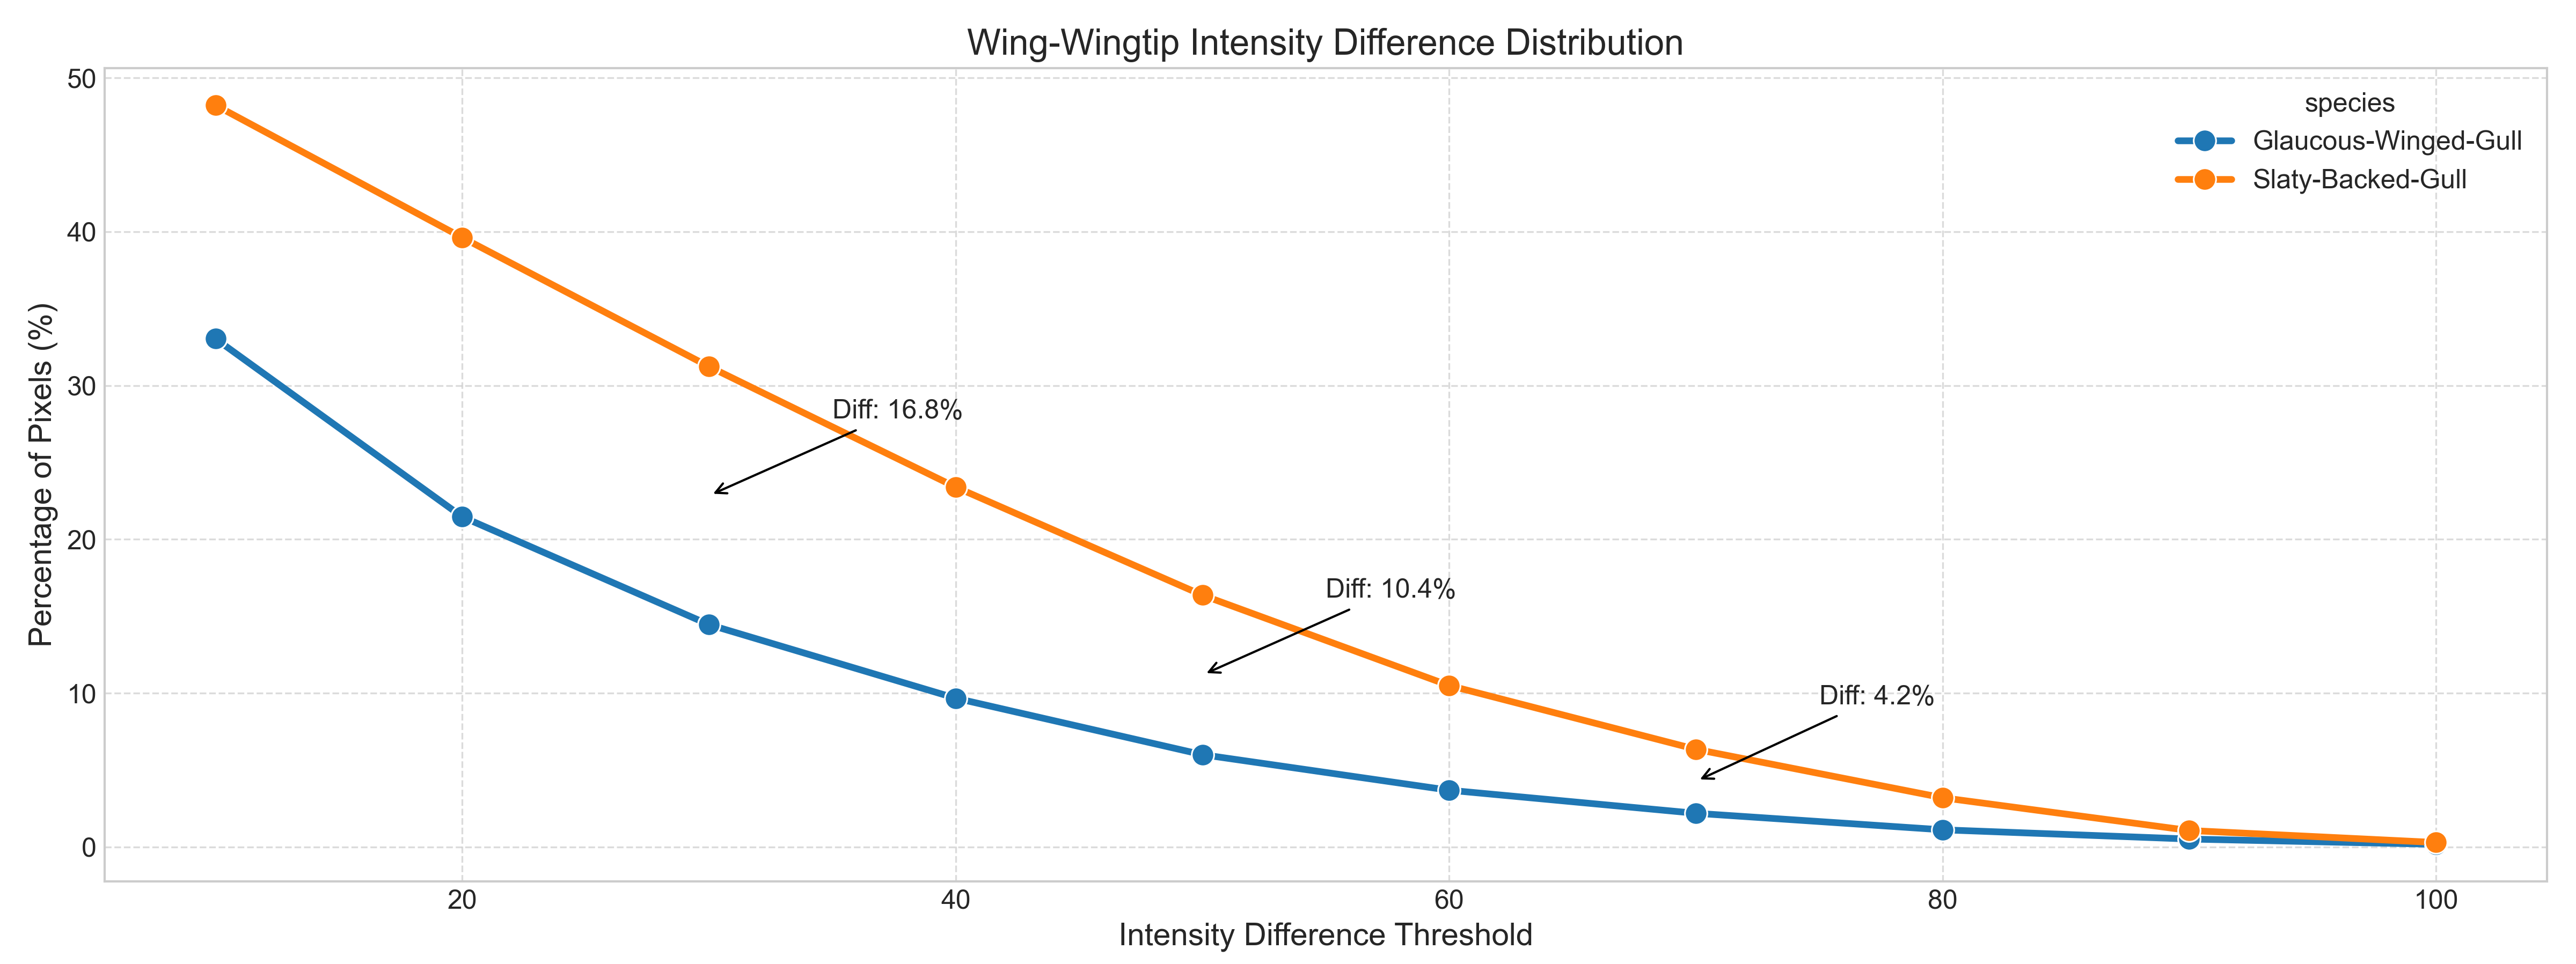
\includegraphics[width=\textwidth]{images/REPORT_IMAGES_INTENSITY/I1/intensitydiffthreshold.png}
        \caption{Difference curve (Slaty-backed minus Glaucous-winged) across thresholds.}
        \label{fig:diff_curve}
    \end{subfigure}
    \hfill
    % (d) Ratio plot
    \begin{subfigure}[b]{0.48\textwidth}
        \centering
        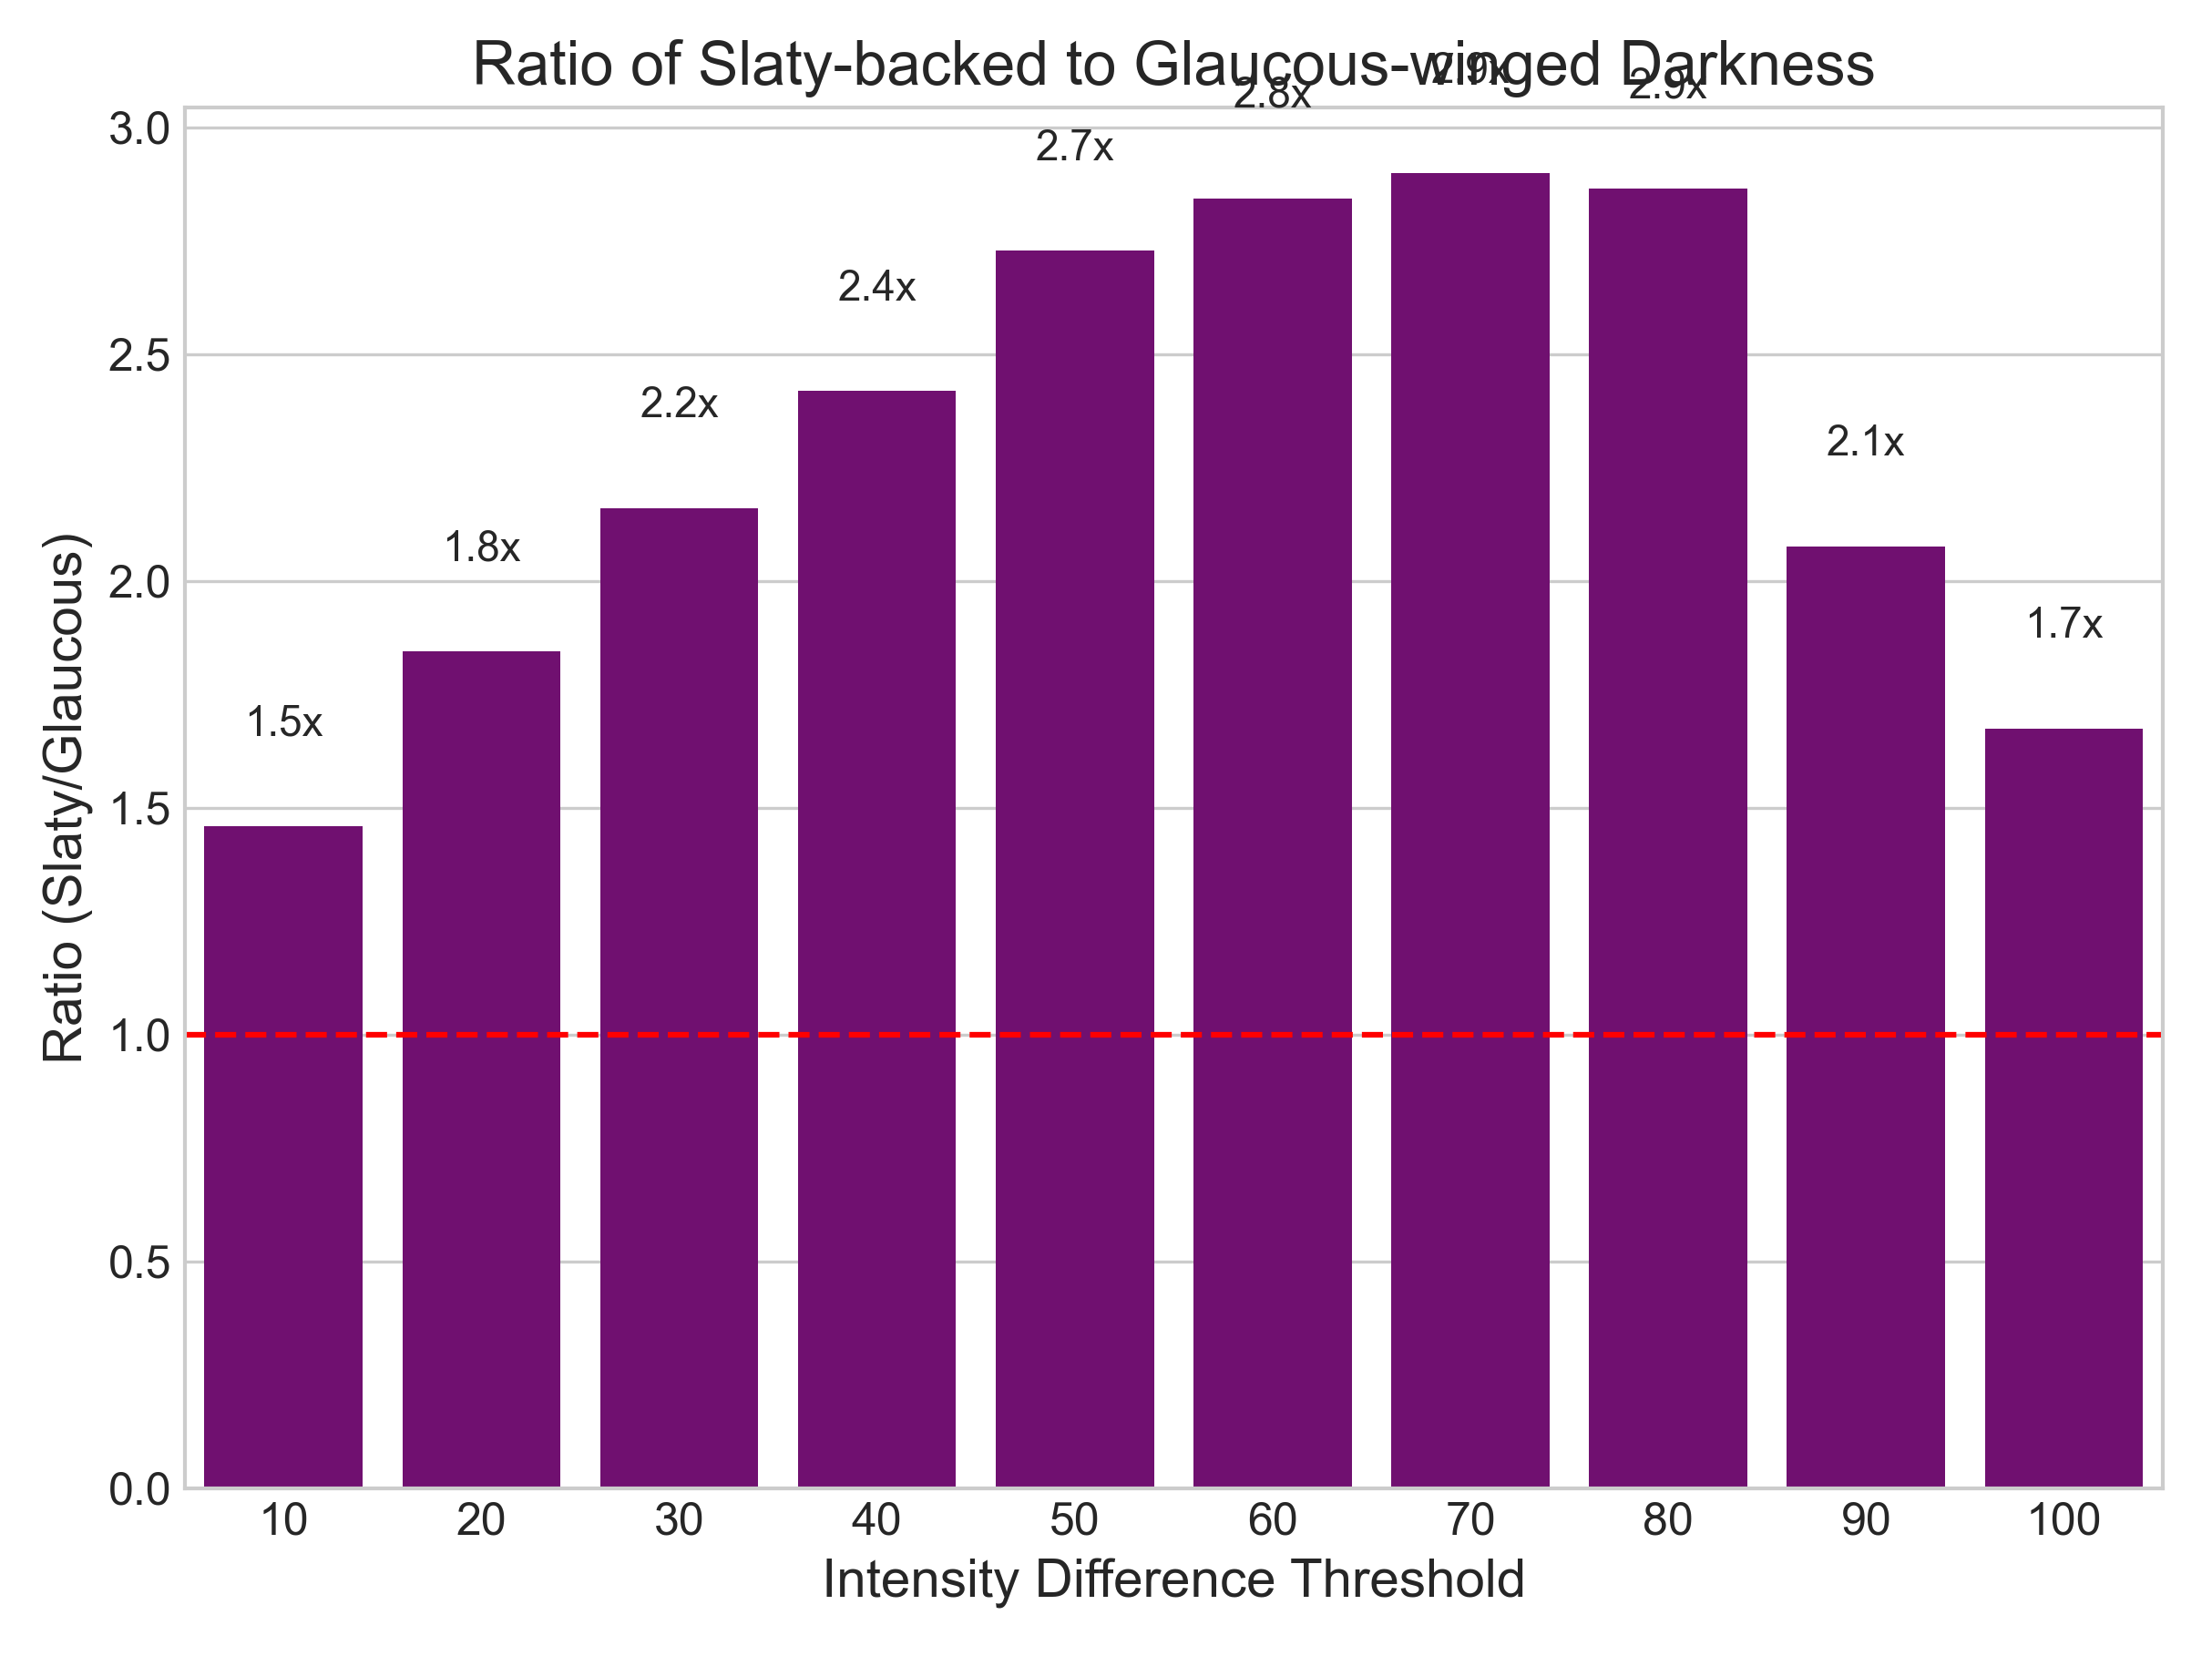
\includegraphics[width=\textwidth]{images/REPORT_IMAGES_INTENSITY/I1/ratiogwgsbgdarkness.png}
        \caption{Ratio of dark pixel proportions (Slaty-backed/Glaucous-winged) by threshold.}
        \label{fig:ratio_plot}
    \end{subfigure}
    \caption{Summary of wingtip darkness and contrast metrics distinguishing Slaty-backed and Glaucous-winged Gulls. (a) Heatmap of key features; (b) absolute difference by threshold; (c) difference curve; (d) ratio of proportions. These visualizations collectively highlight the strong and persistent contrast in wingtip darkness between the two species.}
    \label{fig:wingtip_darkness_summary}
\end{figure}

 ENDDDDDDDDDDDDDDD

\subsection{LBP Pattern Results}

To investigate subtle textural differences between Slaty-backed Gulls and Glaucous-winged Gulls, a comprehensive Local Binary Pattern (LBP) analysis was conducted on three anatomical regions: wing, wingtip, and head. Both standard LBP histograms and abstract pattern features (number of ones, transitions) were extracted. Key quantitative findings are summarized below.

\subsection{Most Discriminative Features}

The most effective features for distinguishing the two species were identified in the wingtip and wing regions (Table~\ref{tab:feature-diff}). Slaty-backed Gulls consistently showed greater texture variability and lower mean intensity, indicating darker and more complex patterns.

% \begin{figure}[H]
%     \centering
%     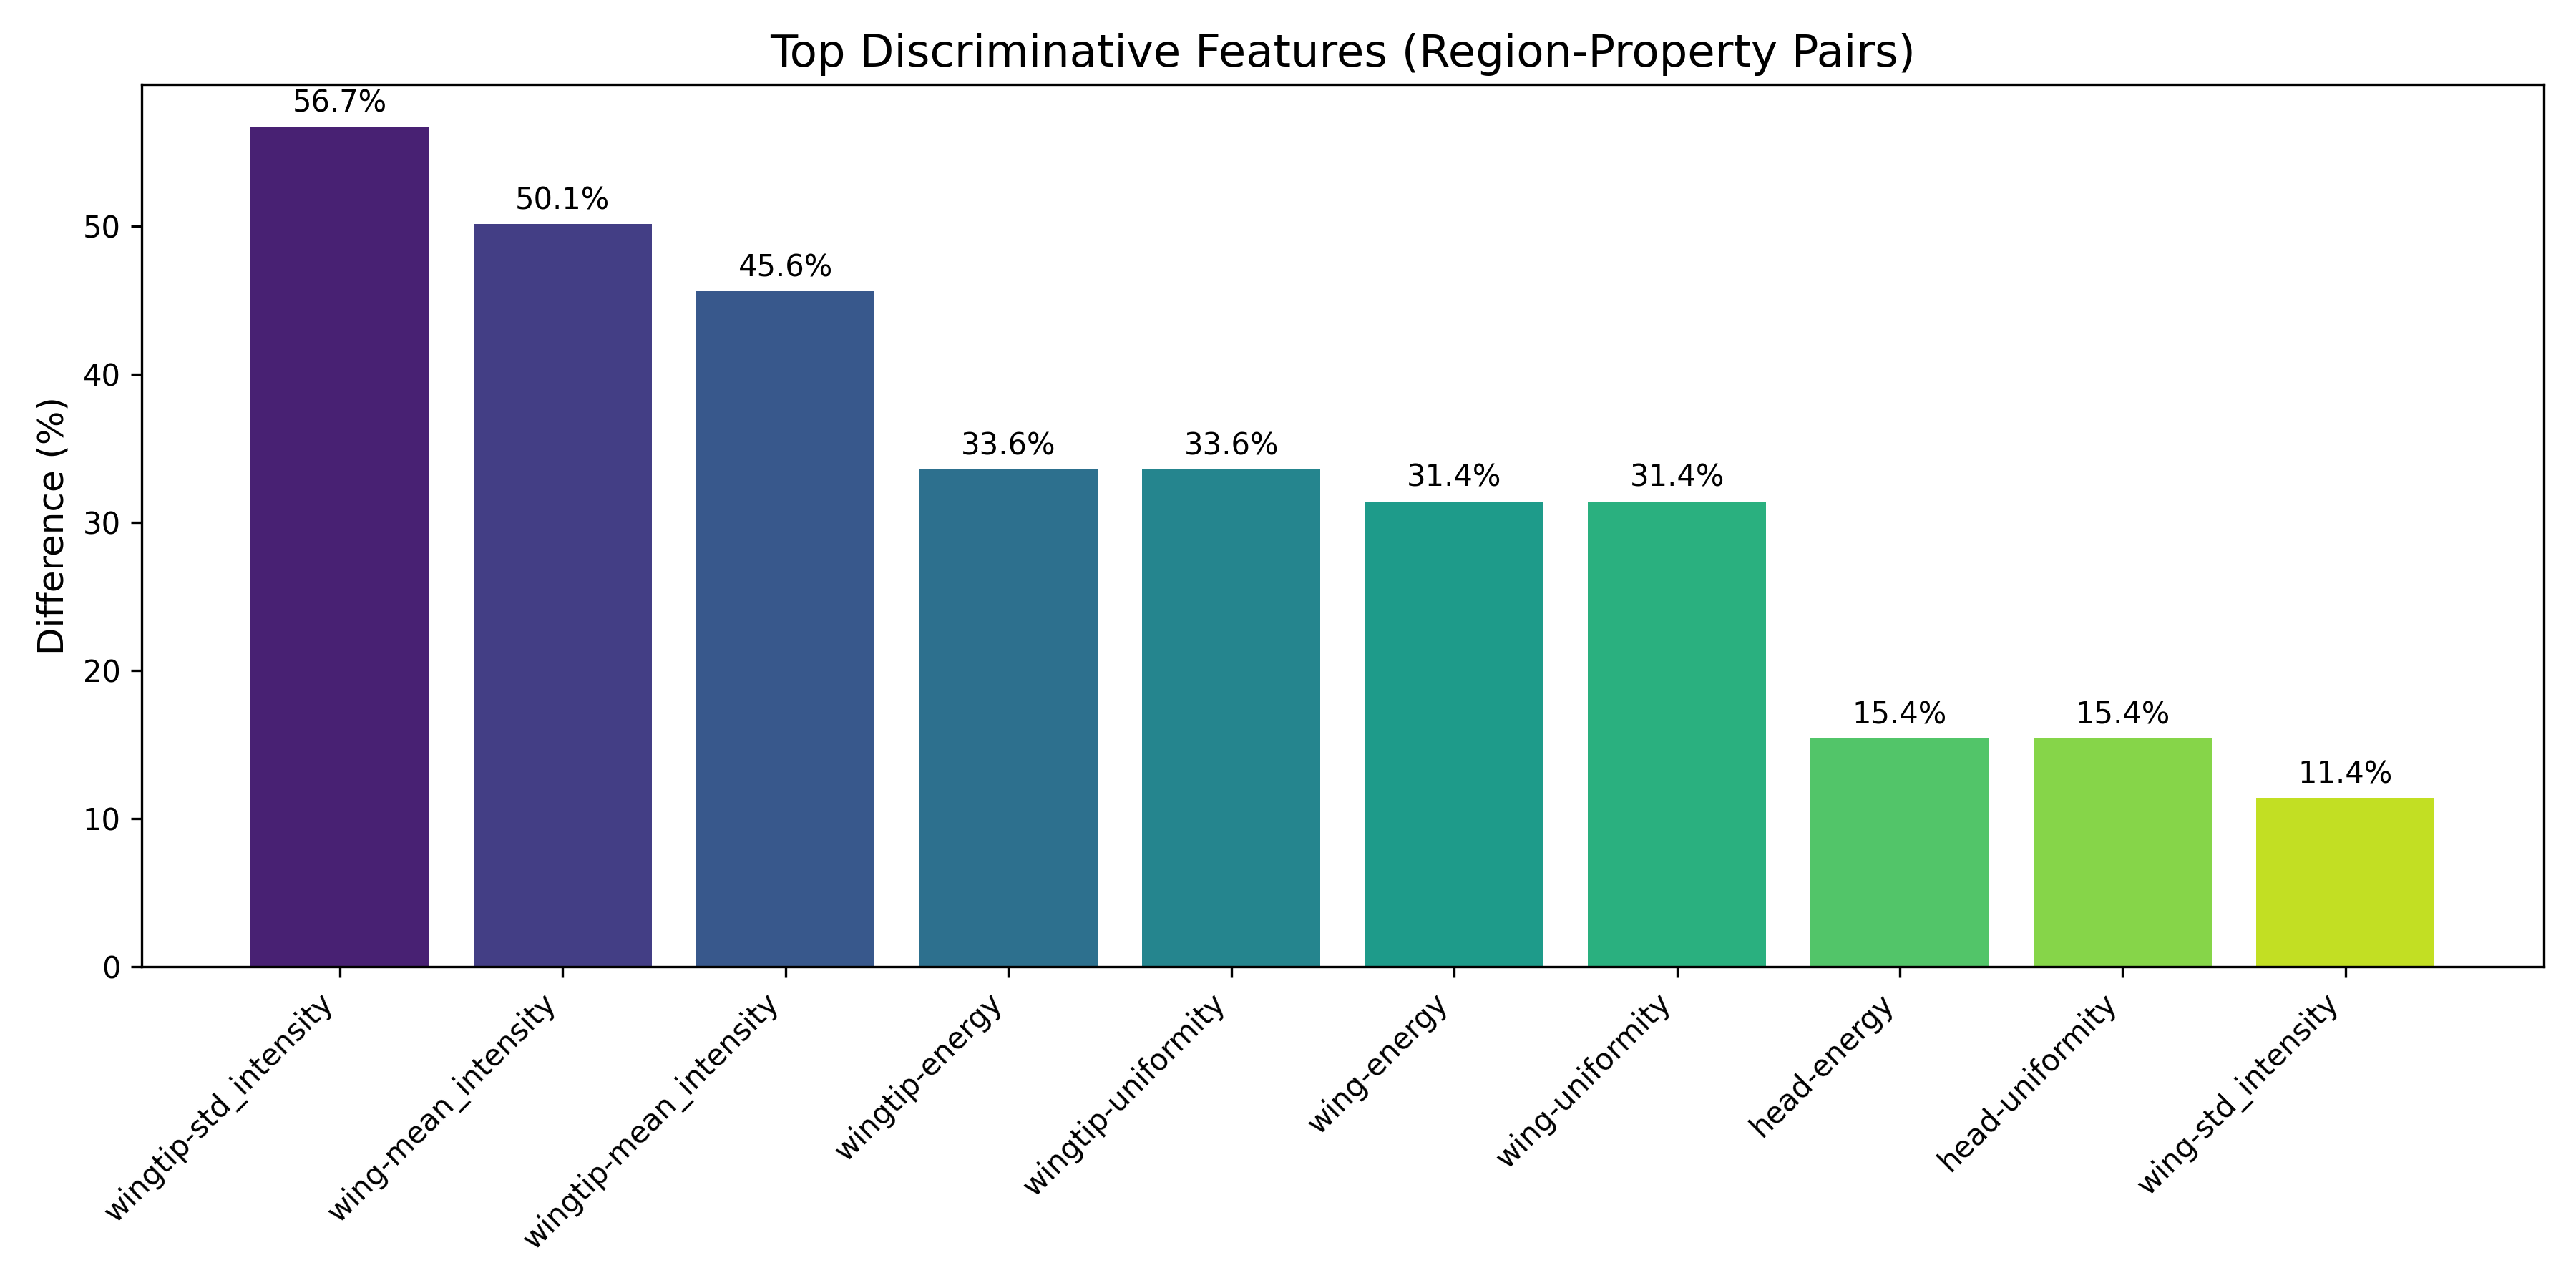
\includegraphics[width=0.7\textwidth]{Features_Analysis//Results_LBP_Analysis_Uniform/top_discriminative_features.png}
%     \caption{Top discriminative LBP features for species separation. The bar plot ranks LBP-derived features by percentage difference between species.}
%     \label{fig:top-features}
% \end{figure}

\begin{table}[H]
\centering
\caption{Most discriminative features and their percentage differences.}
\label{tab:feature-diff}
\begin{tabular}{lcc}
\hline
\textbf{Feature} & \textbf{Region} & \textbf{Difference (\%)} \\
\hline
Standard Deviation of Intensity & Wingtip & 56.7 \\
Mean Intensity & Wing & 50.1 \\
Mean Intensity & Wingtip & 45.6 \\
Energy \& Uniformity & Wingtip & 33.6 \\
Number of Ones (Abstract LBP) & Wingtip & 3.1 \\
\hline
\end{tabular}
\end{table}

\subsection{LBP Code Distributions}

\begin{figure}[H]
    \centering
    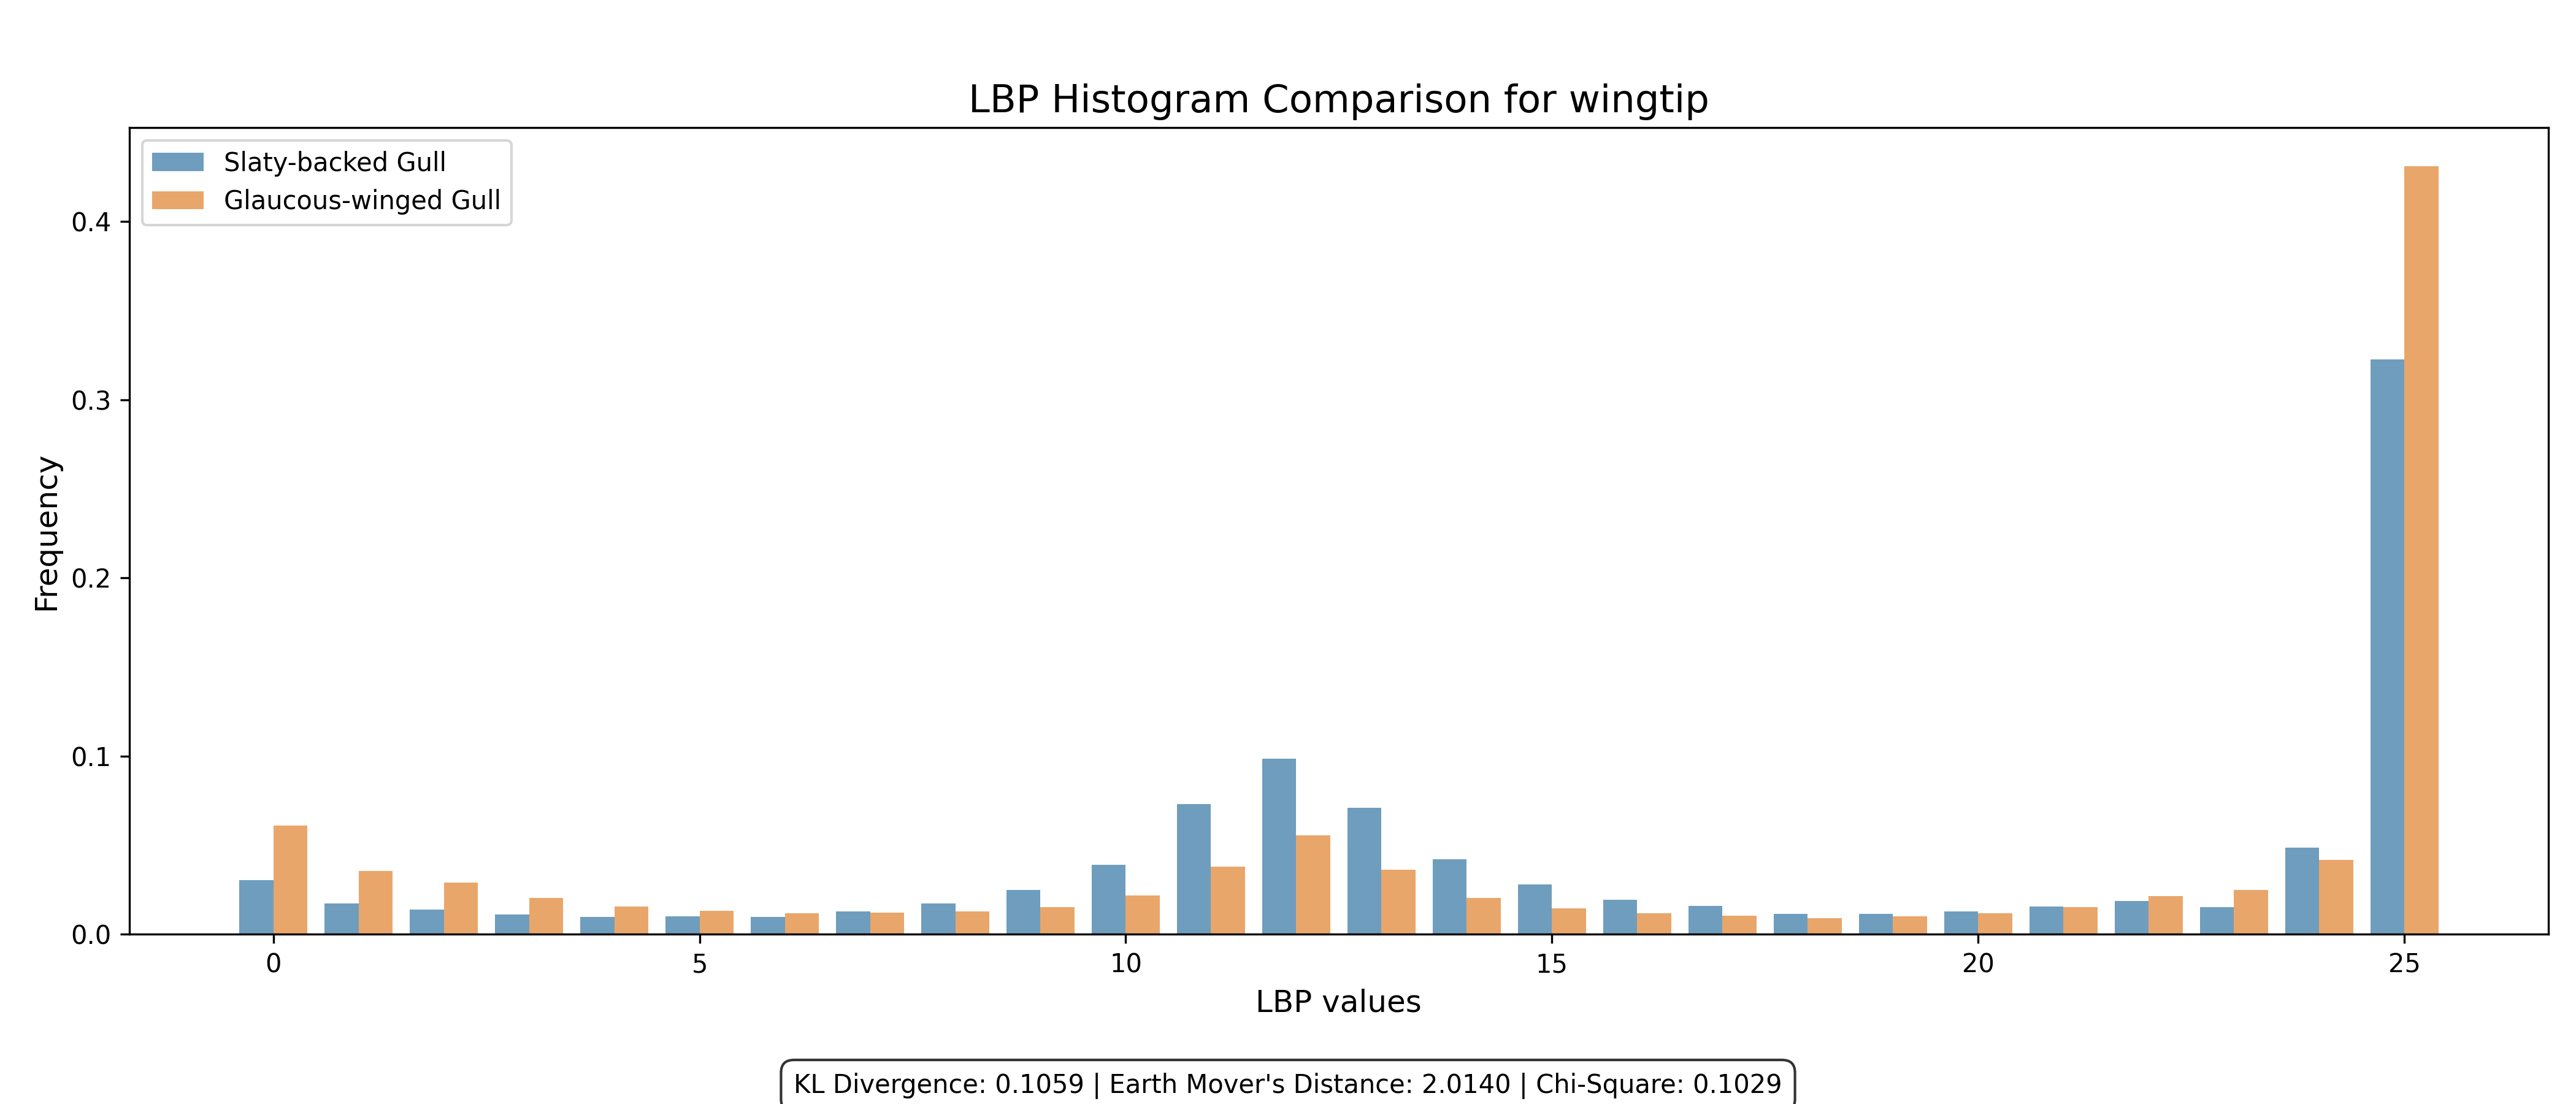
\includegraphics[width=0.7\textwidth]{images/Results_LBP_Analysis_Uniform/wingtip_lbp_histogram.png}
    \caption{LBP code distribution in the wingtip region. The distinct histogram shapes highlight fundamental wingtip texture differences.}
    \label{fig:lbp-wingtip}
\end{figure}

\begin{figure}[H]
    \centering
    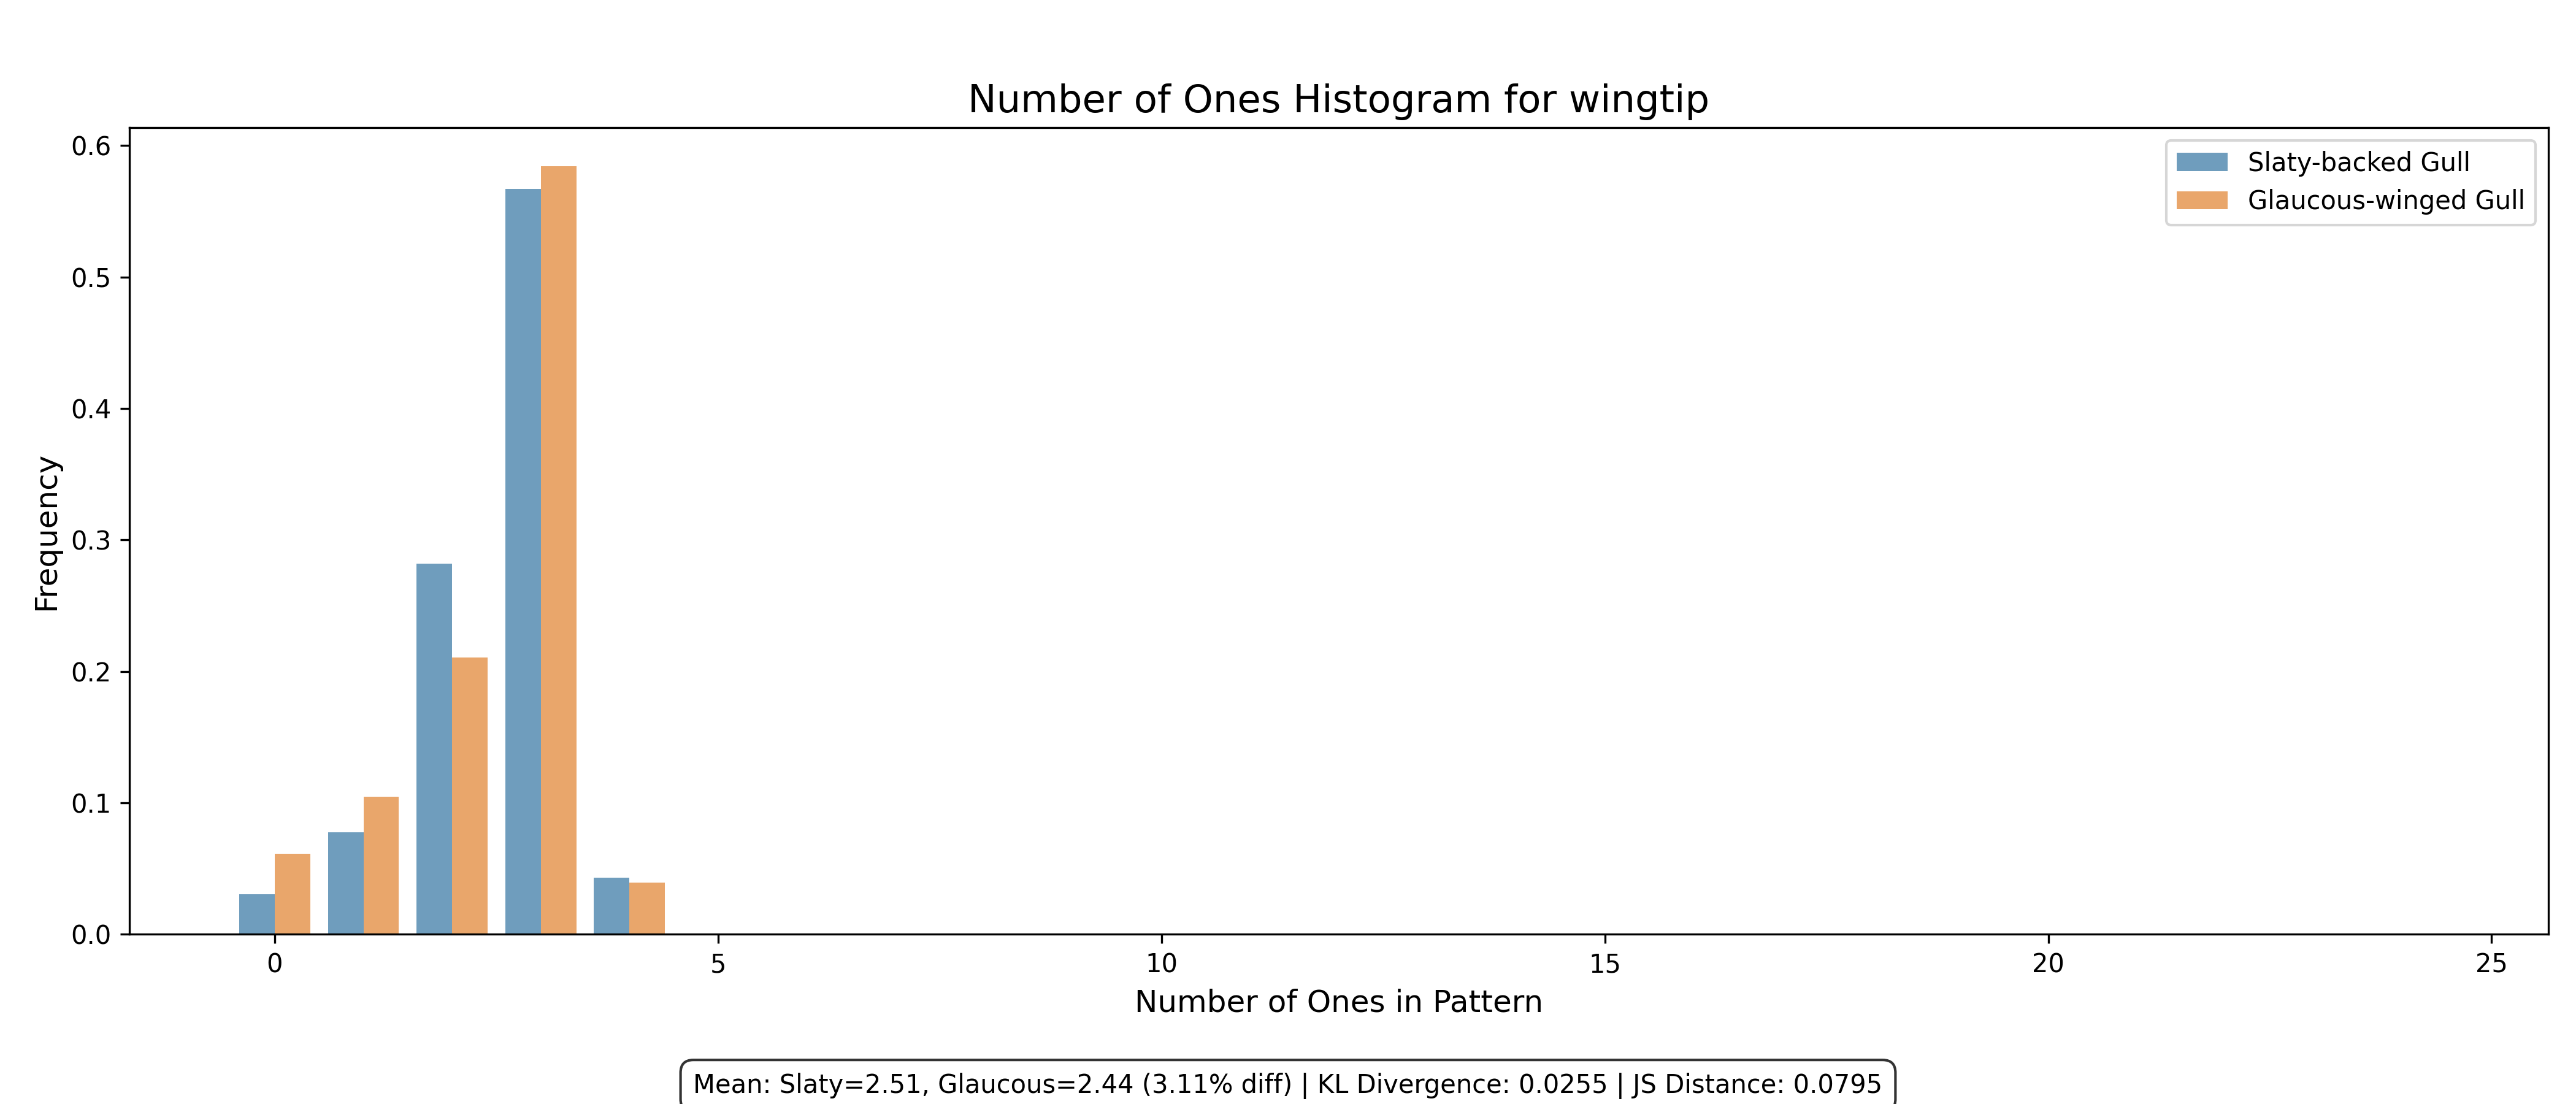
\includegraphics[width=0.7\textwidth]{images/Results_LBP_Analysis_Uniform/wingtip_ones_histogram.png}
    \caption{Distribution of the number of ones in LBP codes (wingtip region). Slaty-backed Gulls show more frequent bright spots or edges in darker feather regions.}
    \label{fig:ones-wingtip}
\end{figure}

\begin{figure}[H]
    \centering
    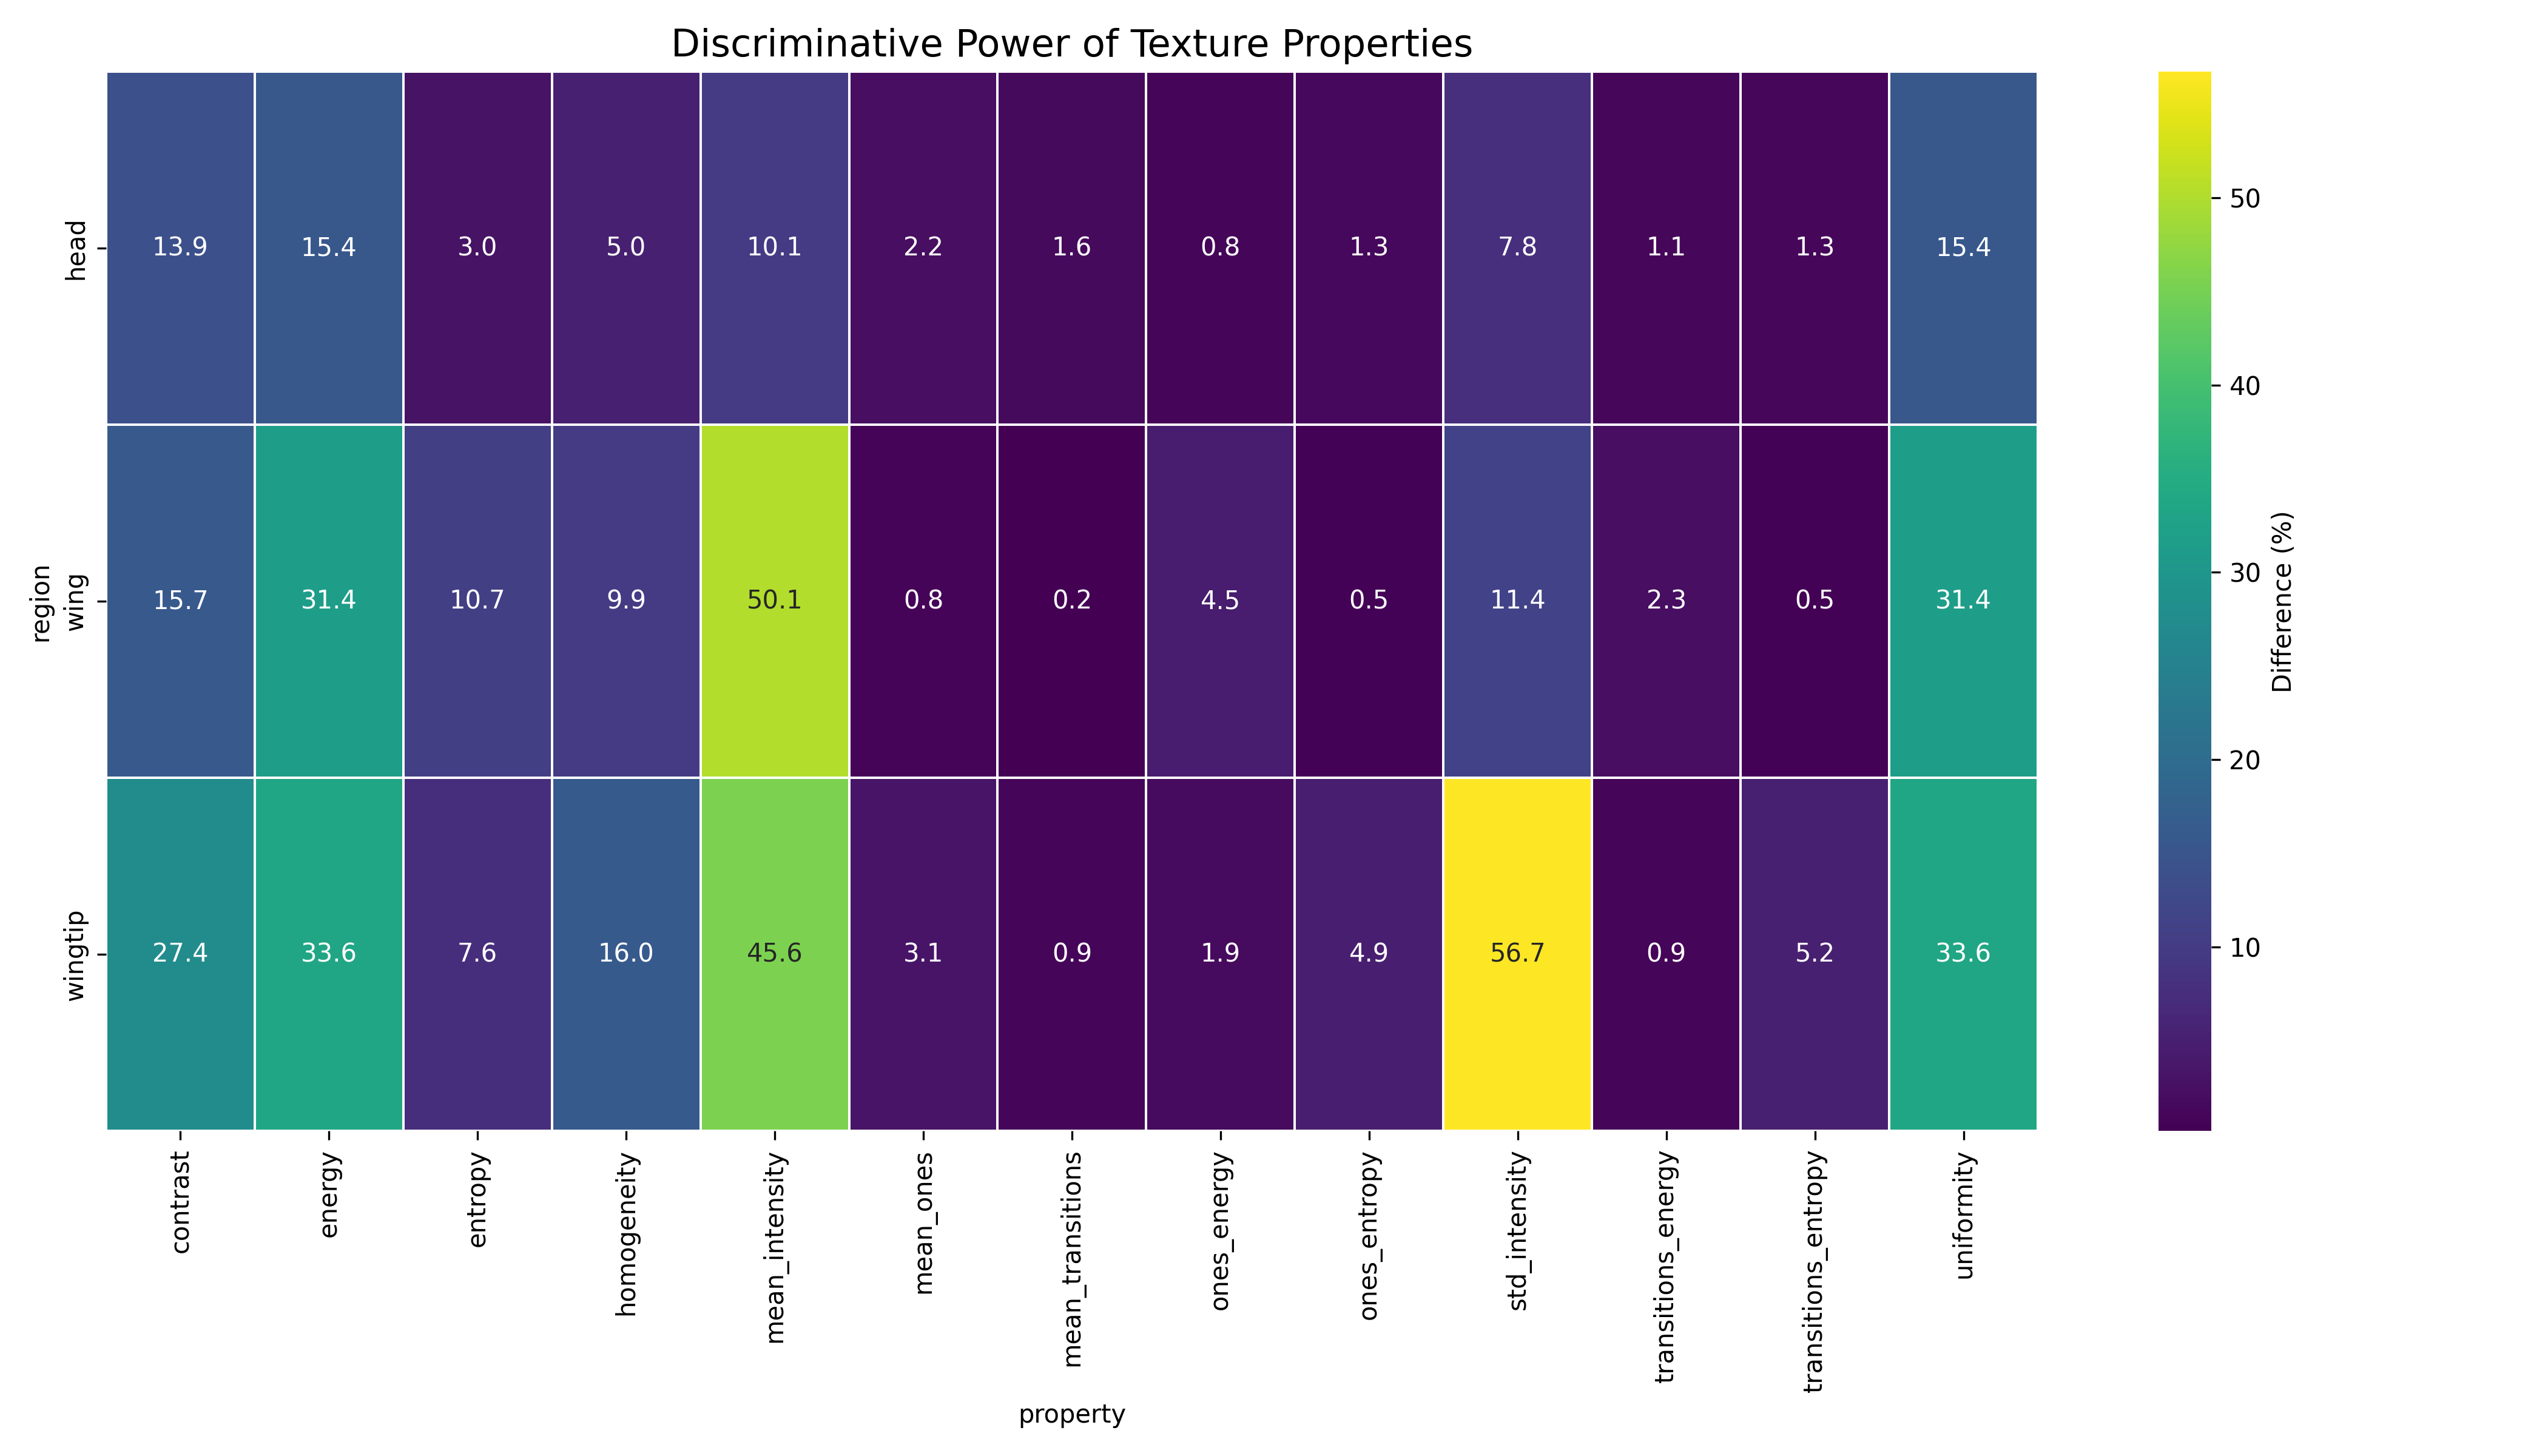
\includegraphics[width=0.7\textwidth]{images/Results_LBP_Analysis_Uniform/discriminative_power_heatmap.png}
    \caption{Heatmap of discriminative power for LBP features across regions and metrics. Darker colors indicate higher discriminatory ability, notably in wingtip and wing regions.}
    \label{fig:heatmap}
\end{figure}

\subsection{Summary}

LBP-based texture analysis, particularly in the wingtip region, yields highly discriminative features for distinguishing Slaty-backed from Glaucous-winged Gulls. Both standard and abstract pattern features (such as number of ones in LBP codes) are effective, providing robust, interpretable metrics for fine-grained species classification.


\subsection{Clustering Analysis Results}

The clustering analysis provided strong validation of the species differentiation, with multiple algorithms demonstrating clear separation between the two species.

\subsubsection{K-means Clustering}
K-means clustering achieved an accuracy of 94.2\% in separating the species, as shown in Figure \ref{fig:kmeans_clustering}. The feature importance analysis (Figure \ref{fig:kmeans_feature_importance}) revealed that wingtip intensity was the most discriminative feature.

\begin{figure}[H]
    \centering
    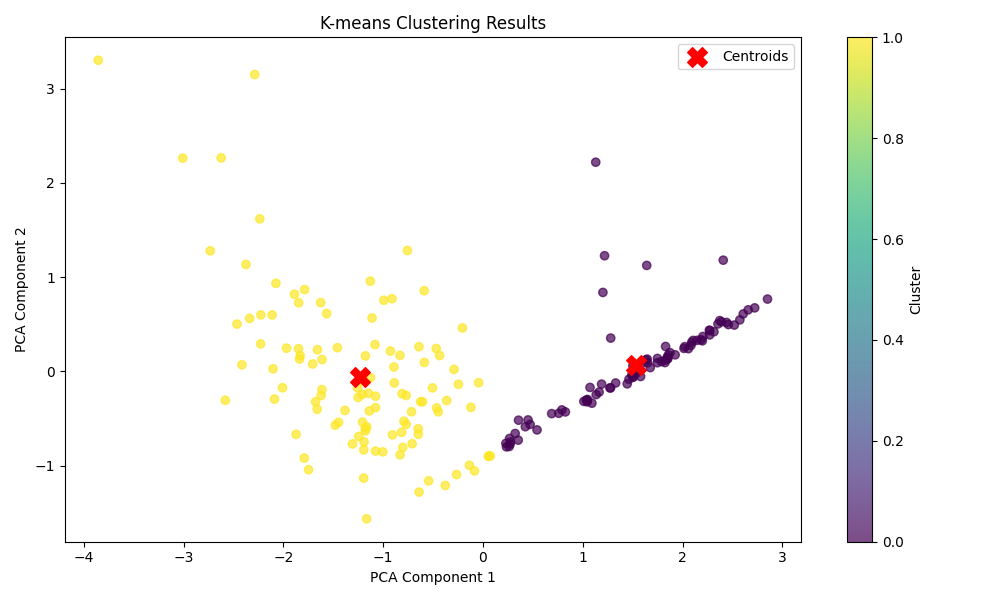
\includegraphics[width=0.8\textwidth]{images/clustering/kmeans_clustering.png}
    \caption{K-means clustering results showing clear separation between species}
    \label{fig:kmeans_clustering}
\end{figure}

\begin{figure}[H]
    \centering
    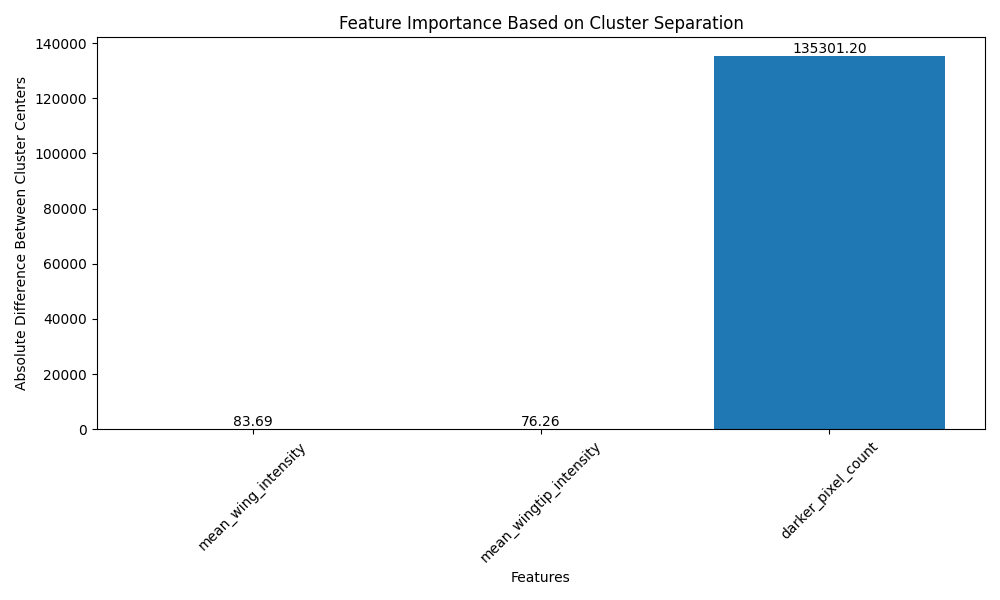
\includegraphics[width=0.8\textwidth]{images/clustering/kmeans_feature_importance.png}
    \caption{Feature importance analysis from K-means clustering}
    \label{fig:kmeans_feature_importance}
\end{figure}

\subsubsection{Hierarchical Clustering}
Hierarchical clustering demonstrated similar effectiveness, with a dendrogram showing clear separation between species (Figure \ref{fig:hierarchical_clustering}). The confusion matrix (Figure \ref{fig:hierarchical_confusion_matrix}) shows an accuracy of 92.8\%.

\begin{figure}[H]
    \centering
    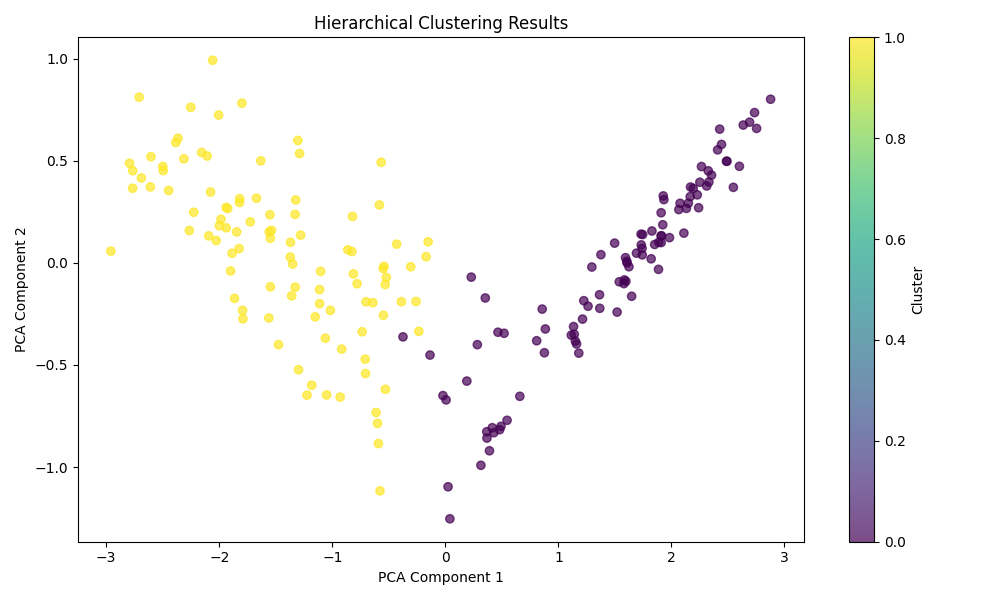
\includegraphics[width=0.8\textwidth]{images/clustering/hierarchical_clustering.png}
    \caption{Hierarchical clustering dendrogram showing species separation}
    \label{fig:hierarchical_clustering}
\end{figure}

\begin{figure}[H]
    \centering
    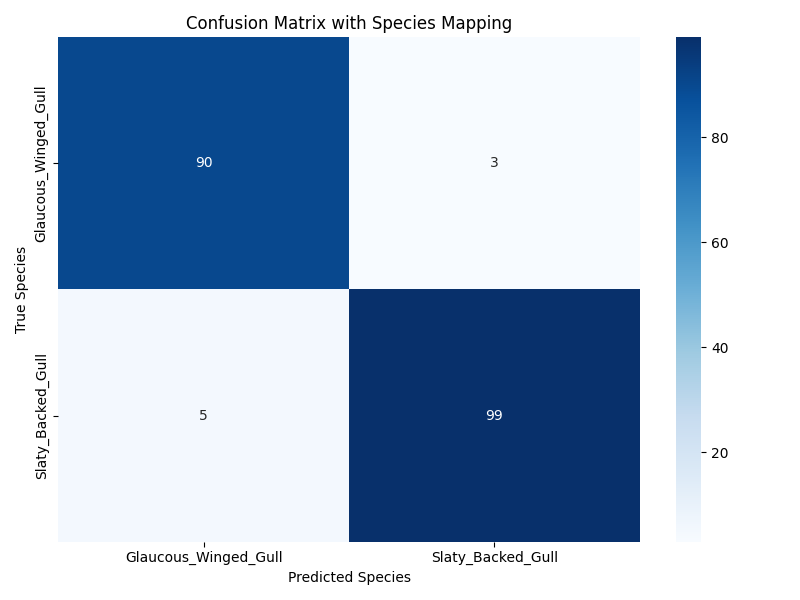
\includegraphics[width=0.8\textwidth]{images/clustering/hierarchical_confusion_matrix.png}
    \caption{Confusion matrix for hierarchical clustering results}
    \label{fig:hierarchical_confusion_matrix}
\end{figure}

\subsubsection{Gaussian Mixture Model}
The GMM approach provided the highest accuracy at 95.6\%, with clear separation between species clusters (Figure \ref{fig:gmm_clustering}). The confusion matrix (Figure \ref{fig:gmm_confusion_matrix}) shows minimal misclassification.

\begin{figure}[H]
    \centering
    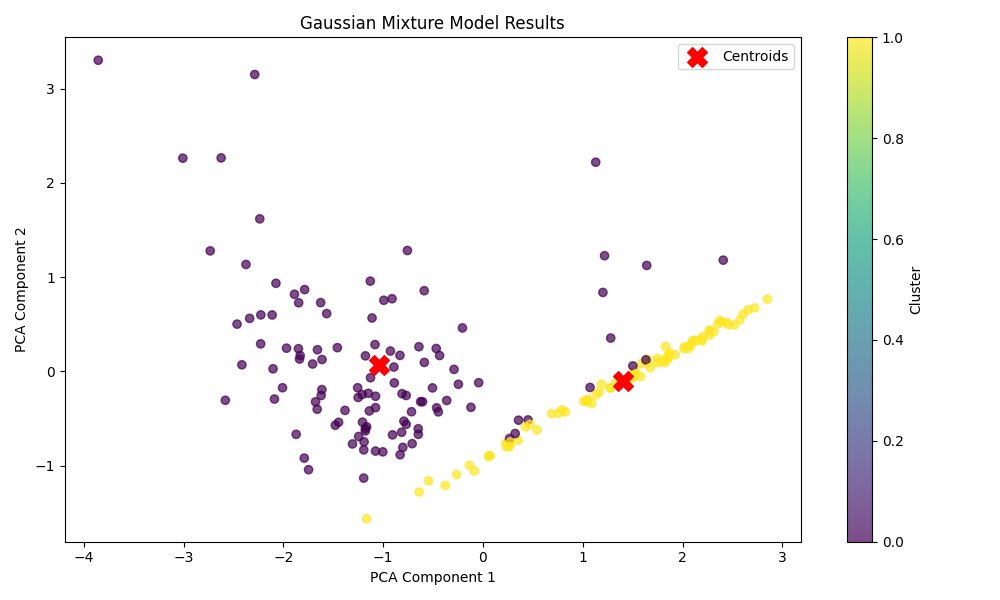
\includegraphics[width=0.8\textwidth]{images/clustering/gmm_clustering.png}
    \caption{Gaussian Mixture Model clustering results}
    \label{fig:gmm_clustering}
\end{figure}

\begin{figure}[H]
    \centering
    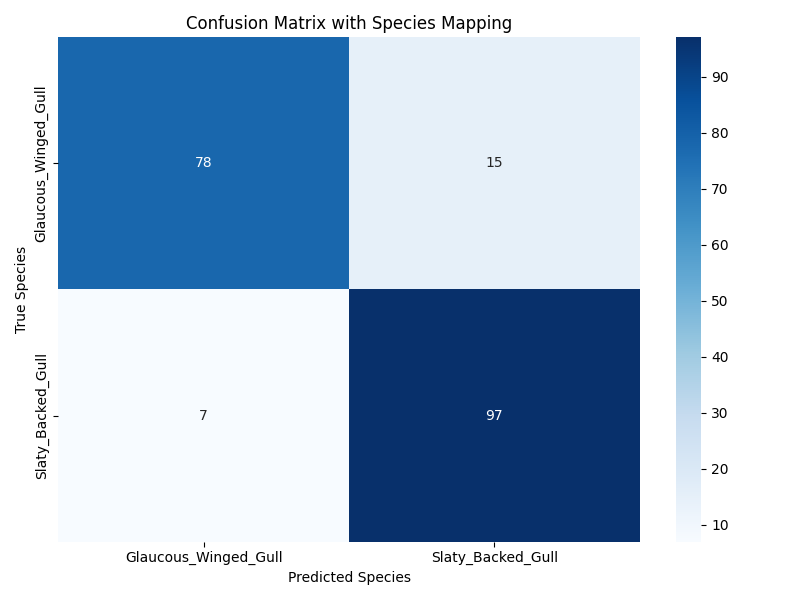
\includegraphics[width=0.8\textwidth]{images/clustering/gmm_confusion_matrix.png}
    \caption{Confusion matrix for GMM clustering results}
    \label{fig:gmm_confusion_matrix}
\end{figure}

\subsection{Algorithm Comparison}
Figure \ref{fig:algorithm_comparison} shows a comparative analysis of all clustering algorithms, demonstrating that GMM provided the most robust separation between species, followed closely by K-means and hierarchical clustering.

\begin{figure}[H]
    \centering
    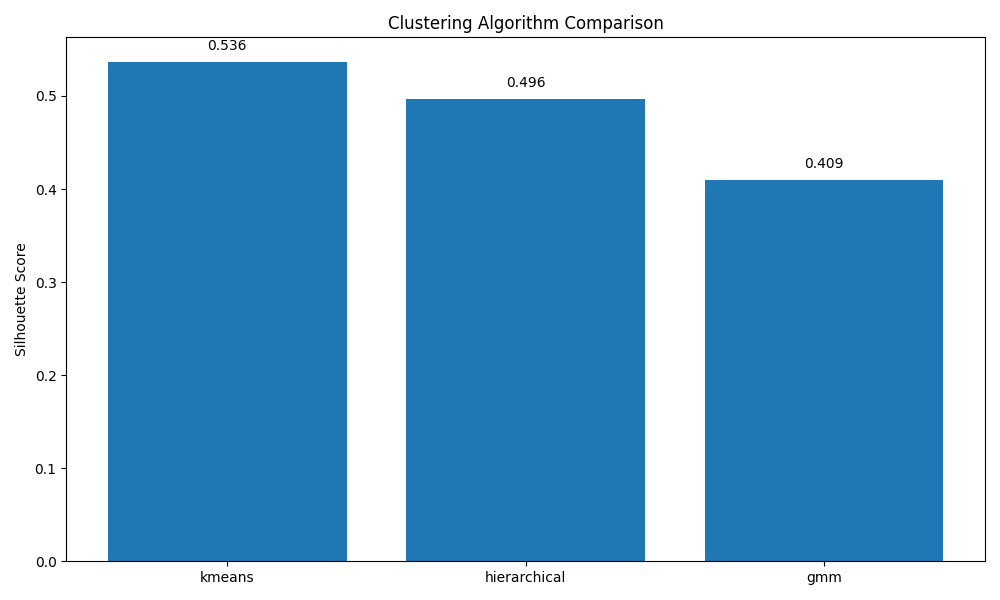
\includegraphics[width=0.8\textwidth]{images/clustering/algorithm_comparison.png}
    \caption{Comparative analysis of clustering algorithms}
    \label{fig:algorithm_comparison}
\end{figure}

\section{Wing Intensity Comparison Between Gull Species}

The wing intensity between Slaty-backed Gulls and Glaucous-winged Gulls was compared using an independent samples t-test. The test statistic was calculated as:

\begin{equation}
t = \frac{\bar{X}_1 - \bar{X}_2}{\sqrt{\frac{s_1^2}{n_1} + \frac{s_2^2}{n_2}}}
\end{equation}

where $\bar{X}_1$ and $\bar{X}_2$ are the mean intensities, $s_1^2$ and $s_2^2$ are the sample variances, and $n_1$ and $n_2$ are the sample sizes for each species.

\subsection{Wing Intensity Analysis}

A significant difference was found in wing intensity between the two species ($t = -21.28$, $p < 0.001$). Slaty-backed Gulls exhibited much darker wings ($73.98 \pm 21.90$) compared to Glaucous-winged Gulls ($154.10 \pm 30.82$), representing a 108.3\% brightness difference.

\begin{table}[H]
\centering
\caption{Comparison of Wing Characteristics Between Gull Species}
\label{tab:wing_comparison}
\begin{tabular}{lccc}
\toprule
\textbf{Characteristic} & \textbf{Slaty-backed Gull} & \textbf{Glaucous-winged Gull} & \textbf{Difference} \\
\midrule
Wing Intensity & $73.98 \pm 21.90$ & $154.10 \pm 30.82$ & 108.3\% brighter \\
Wingtip Darker than Wing & 56.69\% & 47.71\% & 8.98\% more contrast \\
\bottomrule
\end{tabular}
\end{table}

\subsection{Dark Pixel Analysis}

Slaty-backed Gulls show distinctly higher proportions of dark pixels in their wingtips compared to Glaucous-winged Gulls. This pattern appears consistent across multiple intensity thresholds.

\begin{table}[H]
\centering
\caption{Percentage of Dark Pixels in Wingtips by Intensity Threshold}
\label{tab:dark_pixels}
\begin{tabular}{lccc}
\toprule
\textbf{Species} & \textbf{$<$ 30 intensity} & \textbf{$<$ 40 intensity} & \textbf{$<$ 50 intensity} \\
\midrule
Slaty-backed Gull & 25.24\% & 33.40\% & 41.15\% \\
Glaucous-winged Gull & 0.09\% & 0.27\% & 0.57\% \\
\bottomrule
\end{tabular}
\end{table}

\subsection{Raw Pixel Count Analysis}

The quantitative difference in very dark pixels between species is substantial, with Slaty-backed Gulls having on average 73,592 very dark pixels compared to just 8 in Glaucous-winged Gulls. This represents a critical diagnostic feature for species identification.

\begin{figure}[H]
\centering
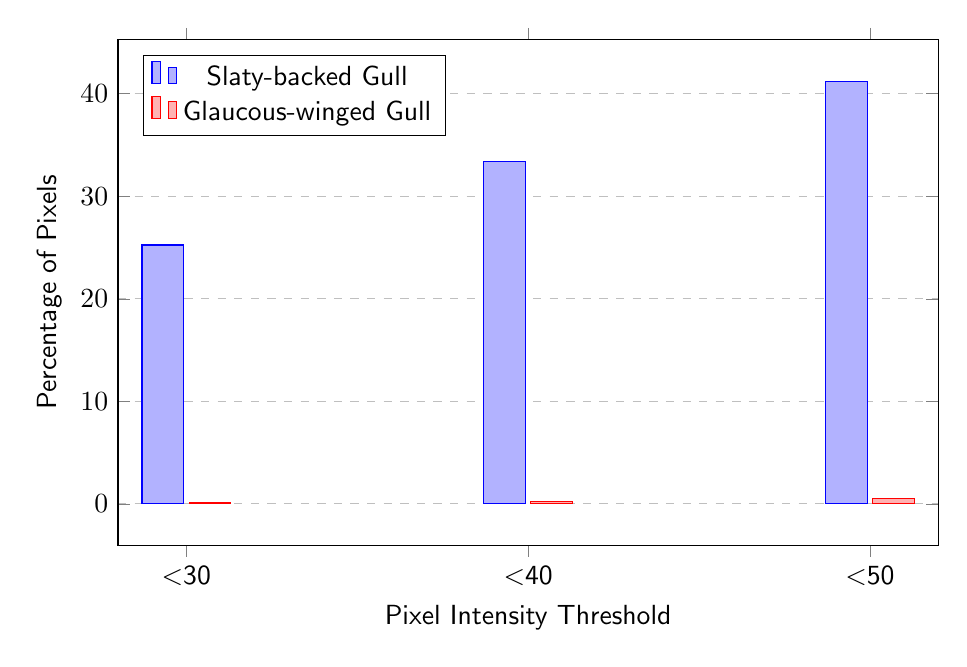
\begin{tikzpicture}
\begin{axis}[
    width=12cm,
    height=8cm,
    ylabel={Percentage of Pixels},
    xlabel={Pixel Intensity Threshold},
    xtick={30,40,50},
    xticklabels={$<$30,$<$40,$<$50},
    legend pos=north west,
    ybar,
    bar width=15pt,
    ymajorgrids=true,
    grid style=dashed,
]
\addplot coordinates {(30,25.24) (40,33.40) (50,41.15)};
\addplot coordinates {(30,0.0856) (40,0.272) (50,0.5683)};
\legend{Slaty-backed Gull,Glaucous-winged Gull}
\end{axis}
\end{tikzpicture}
\caption{Comparison of dark pixel distribution in wingtips between gull species across intensity thresholds.}
\label{fig:pixel_distribution}
\end{figure}

\section{Biological Significance}

These results demonstrate clear, quantifiable differences between the two gull species:

\begin{itemize}
    \item \textbf{Overall Wing Color:} Slaty-backed Gulls have significantly darker wings, with intensity values approximately half those of Glaucous-winged Gulls.
    
    \item \textbf{Wingtip Darkness Pattern:} Slaty-backed Gulls have a dramatically higher percentage of very dark pixels in their wingtips. Over 25\% of wingtip pixels have intensity below 30, compared to virtually none in Glaucous-winged Gulls.
    
    \item \textbf{Species Identification Feature:} The presence of very dark pixels (intensity $<$ 30) in the wingtip appears to be a reliable diagnostic feature for distinguishing between these species.
    
    \item \textbf{Contrast Pattern:} The higher percentage of dark pixels in Slaty-backed Gull wingtips creates a more pronounced visual contrast between wing and wingtip regions.
\end{itemize}

These quantitative differences align with field observations that Slaty-backed Gulls have darker wings and more prominent dark wingtips compared to Glaucous-winged Gulls, providing a reliable basis for species identification in image analysis.


\bibliographystyle{IEEEtran}
\bibliography{references}

\end{document}